\documentclass[11pt,a4book,openany,dvipdfmx]{book}

\usepackage{ulem} 
\usepackage[abs]{overpic}
\usepackage{tikz}
\usepackage{tikz-feynhand}

\usepackage[labelformat=empty,labelsep=none]{caption} % figure のキャプション Figure: を消去




\title{$d(K^-, n K^0)"n"$ Analysis}
\subtitle{バックグラウンドを差し引いた断面積}

\author{井上謙太郎}




\newcommand{\tmp}[1]{\textcolor{red}{\bf #1}}


\newcommand{\IMfitChiSquare}{1077.4}
\newcommand{\IMfitNDF}{352}
\newcommand{\IMfitChiNDF}{3.06}

\newcommand{\KzeroFitChi}{275.2}
\newcommand{\KzeroFitNDF}{43}
\newcommand{\KzeroFitChiNDF}{6.40}

\newcommand{\KzeroOneStepRatio}{80.9 \pm 1.3\%}
\newcommand{\KzeroTwoStepRatio}{11.5 \pm 1.0\%}
\newcommand{\KzeroLsRatio}{7.7 \pm 0.6\%}

\newcommand{\fitScatLength}{-1.05 \pm 0.12 (fit.) \pm +0.09 (syst.) + [ 0.86 \pm 0.15 (fit.) ^{+0.07} _{-0.08} (syst.)]i}
\newcommand{\fitEffRange}{-0.22 \pm 0.40 (fit.) ^{+0.05} _{-0.06} (syst.) + [ -0.42 \pm 0.16 (fit.) ^{+0.12} _{-0.08} (syst.)]i}
\newcommand{\fitPole}{1418.3 ^{+7.5} _{-2.4} (fit.)^{+0.9}_{-1.1} (syst.)}
\newcommand{\fitWidth}{-27.8^{+9.5}_{-0.9} (fit.)^{+1.9}_{-2.1} (syst.)}

\newcommand{\fitAscaleIz}{0.562 \pm 0.015}
\newcommand{\fitAscaleIo}{1.070 \pm 0.040}
\newcommand{\fitAscaleIzVal}{0.562}
\newcommand{\fitAscaleIzErr}{0.015}
\newcommand{\fitAscaleIoVal}{1.070}
\newcommand{\fitAscaleIoErr}{0.040}
\newcommand{\fitAscaleChi}{691/42}
\newcommand{\fitAscaleChiNum}{16.4}

\newcommand{\fitBscaleIz}{0.721 \pm 0.016}
\newcommand{\fitBscaleIo}{1.423 \pm 0.055}
\newcommand{\fitBscaleIzVal}{0.721}
\newcommand{\fitBscaleIoVal}{1.423}
\newcommand{\fitBscaleIzErr}{0.016}
\newcommand{\fitBscaleIoErr}{0.055}
\newcommand{\fitBscaleChi}{220/42}
\newcommand{\fitBscaleChiNum}{5.25}

\newcommand{\fitBBChi}{187/41}
\newcommand{\fitBBChiNum}{4.56}
\newcommand{\fitBBIz}{0.686 \pm 0.017}
\newcommand{\fitBBIo}{1.462 \pm 0.059}
\newcommand{\fitBBphase}{0.828 \pm 0.030}
\newcommand{\fitBBIzVal}{0.686}
\newcommand{\fitBBIoVal}{1.462}
\newcommand{\fitBBphaseVal}{0.828}
\newcommand{\fitBBIzErr}{0.017}
\newcommand{\fitBBIoErr}{0.059}
\newcommand{\fitBBphaseErr}{0.030}
\newcommand{\fitBBDegree}{34.1^{+3.0}_{-3.2}}

\newcommand{\fitBChi}{184/41}
\newcommand{\fitBChiNum}{4.48}
\newcommand{\fitBIz}{0.682 \pm 0.017}
\newcommand{\fitBIo}{1.570 \pm 0.058}
\newcommand{\fitBphase}{0.811 \pm 0.030}
\newcommand{\fitBIzVal}{0.682}
\newcommand{\fitBIoVal}{1.570}
\newcommand{\fitBphaseVal}{0.811}
\newcommand{\fitBIzErr}{0.017}
\newcommand{\fitBIoErr}{0.058}
\newcommand{\fitBphaseErr}{0.030}
\newcommand{\fitBDegree}{35.8^{+2.8}_{-3.1}}

\newcommand{\fitScaleKN}{0.0372 \pm 0.0047}
\newcommand{\fitAreKN}{-1.05 \pm 0.12}
\newcommand{\fitAimKN}{ 0.86 \pm 0.15}
\newcommand{\fitRreKN}{-0.22 \pm 0.40}
\newcommand{\fitRimKN}{ 0.42 \pm 0.16}
\newcommand{\fitKNMass}{1418.3}
\newcommand{\fitKNWidth}{27.8}

\newcommand{\fitScaleKmp}{0.0377 \pm 0.0042}
\newcommand{\fitAreKmp}{-0.95 \pm 0.11}
\newcommand{\fitAimKmp}{ 0.94 \pm 0.16}
\newcommand{\fitRreKmp}{-0.27 \pm 0.40}
\newcommand{\fitRimKmp}{ 0.52 \pm 0.18}
\newcommand{\fitKmpMass}{1417.6}
\newcommand{\fitKmpWidth}{30.3}

\newcommand{\fitScaleKzeroN}{0.0367 \pm 0.0053}
\newcommand{\fitAreKzeroN}{-1.13 \pm 0.13}
\newcommand{\fitAimKzeroN}{ 0.79 \pm 0.15}
\newcommand{\fitRreKzeroN}{-0.16 \pm 0.40}
\newcommand{\fitRimKzeroN}{ 0.33 \pm 0.16}
\newcommand{\fitKzeroNMass}{1419.3}
\newcommand{\fitKzeroNWidth}{25.9}



\begin{document}
\maketitle
\tableofcontents

\chapter{Introduction} \label{chapter:Introduction}
%% \section{$\Lambda(1405)$ and $\bar{K}N$ interaction} \label{sec:intro_history}
%% \section{History of the $\Lambda(1405)$}
The $\Lambda(1405)$ is a hyperon containing strangeness $S=-1$ with isospin $I=0$ and spin and spin-parity $J^P=(\frac{1}{2})^-$.
In the latest particle data group (PDG) \cite{PDG}, the mass and the width of the $\Lambda(1405)$ are assigned to $1405.1^{+1.3}_{-1.0}$MeV and $50.5\pm 2.0$MeV respectively,
based on several articles \cite{Dalitz, HADES_pheno, Esmaili}. 

The existance of the $\Lambda(1405)$ was first predicted by Dalitz and Taun in 1959 as the quasi-bound state of the $\bar{K}N$ \cite{Dalitz_1st}.
At the Lawrence Radiation Laboratory,
a $\Lambda(1405)$-like excess state was observed in 1961 by the bubble chamber in the $\pi\Sigma$ spectrum using the $K^- p\rightarrow\Sigma \pi \pi \pi$ reaction\cite{L1405_LRL}.
They reported a $\Lambda(1405)$-like excess state in the neutral $\pi\Sigma$ spectrum against to the double charged spectrum, for example $\pi^-\Sigma^-$ or $\pi^+ \Sigma^+$ spectra.
Hemingway reported the successful high-statistics production of $\Lambda(1405)$ by a hydrogen bubble chamber using a $4.2$ GeV $K^-$ beam\cite{Hemingway}.
They claimed that the identification of the $K^- p \rightarrow \pi \Sigma(1660) \rightarrow \pi \pi \Lambda(1405) \rightarrow \pi \pi (\pi \Sigma)$ reaction lemma
enhanced the production of the $\Lambda(1405)$.
Dalitz and Deloff applied M-matrix/K-matrix analysis to the $\pi^-\Sigma^+$ spectrum, which is expected to be background-free from non-resonant and $\Lambda(1520)$ in this data,
and evaluated the mass and width of $\Lambda(1405)$ at $1406.4 \pm 4.0$MeV and $50\pm 2$MeV, respectively\cite{Dalitz}.
This data is employed PDG's estimation for the mass and width of $\Lambda(1405)$.

In the 2000's, the chiral unitary model claimed that the $\Lambda(1405)$ is a dynamical molecular state contributed from two poles,
$\pi\Sigma$ in the low-mass region and $\bar{K}N$ in the high-mass region.
According to the this model, the high-mass pole coupled to $\bar{K}N$ is $1426+16$MeV and the low-mass pole coupled to $\pi\Sigma$ is $1390+66i$MeV.
That means the $\pi \Sigma$ spectrum is expected to shift high mass region from the conventional $1405$MeV by directly accessing to the $\bar{K}N$ pole.

Experimentally, the $\Lambda(1405)$ production was also carried out employing various reaction mechanisms.

B.Riley et. el. reported $\Sigma^{\pm}\pi^{\mp}$ invariant mass of
$K^{-} {}^4\mbox{He} \rightarrow \pi^{\pm} \Sigma^{\mp}$ at rest reaction by stopped $K^-$ using the bubble chamber at Argonne National Laboratory.
The analysis by Esmaili et al. based on this experimental results is employed PDG's estimation of the mass of $\Lambda(1405)$ \cite{Esmaili}.

Niiyama et el. performed photoproduction $\gamma p \rightarrow K^+ \Lambda(1405)$ employing a $\gamma$ beam at $E_{\gamma}=1.5-2.4$GeV at the LEPS beamline in the Spring-8\cite{Niiyama}.
They measured the scattering angle in center of mass system of $K^+$ at $0.8<\Theta_{K^+}<1.0$,
reported mass spectra of $\pi^-\Sigma^+$ and $\pi^+\Sigma^-$ in the $\Lambda(1405) \rightarrow \pi \Sigma$ decay
and observed a difference between the two spectra in the $\Lambda(1405)$ region.
This fact means existance of the interference term between the isospin $I=0$ and $I=1$ channel.
The CLAS collaboration employing a $1.61$-$1.91$GeV $\gamma$ beam for photoproduction at the Jefferson Labolatory
and measured the scattering angle in center of mass system of $K^+$ at $0.6<\Theta_{K^+}<0.9$ \cite{CLAS,CLAS2}.
They reported all three $\pi^-\Sigma^+$, $\pi^+\Sigma^-$ and $\Sigma^0\pi^0$ spectra.
The centroid of those three spectra appear to be at $1405$MeV, but their lineshapes are different indicating contribution of $I=1$ strength in this reaction.

The HADES collaboration performed $\Lambda(1405)$ production in p-p collisions using the $3.5\mbox{GeV}/c$ proton beam \cite{HADES}.
They reported $\pi^-\Sigma^+$, $\pi^+\Sigma^-$ and these average spectra, which clearly show a peak below $1400$MeV.
The analysis by Hassanvand et al. based on this experimental results is employed PDG's estimation of the mass and the width of $\Lambda(1405)$ \cite{HADES_pheno}.

Therefore, the spectrum of $\Lambda(1405)$ depends on the reaction mechanism and the $\pi\Sigma$ charge state for $\Lambda(1405) \rightarrow \pi \Sigma$.
This strongly suggests that $\Lambda(1405)$ is a dynamic state, but the mechanism of these reactions is still controversial and its structure is unknown.

%% \section{$d(K^-, n)$ reaction}
%% \begin{frame}{$d(K^-, n)$ reaction and J-PARC E31}
  \begin{tabular}{cc}
    \begin{minipage}{0.65\hsize}
      Using bubble chamber at the CERN by Braun \cite{Braun}. \\
      $\blacktriangleright$ 686-848 $MeV/$c $K^-$ beam. \\
      $\blacktriangleright$ Wide angle of $n$ was measured. \\
      $\Rightarrow$ Diag.(a) is considered to be dominant. \\
      
      J-PARC E31 experiment\\
      $\blacktriangleright$ 1.0 $GeV/$c $K^-$ beam. \\
      $\blacktriangleright$ Super-forward neutron was measured. \\
      $\Rightarrow$ Diag.(b) is considered to be dominant.
      
      \begin{thebibliography}{99}
        \scriptsize
      \bibitem{Braun} \href{https://www.sciencedirect.com/science/article/pii/0550321377900153}
        {O. Braun et el., Nucl. Phys. B {\bf 129}, 1 (1977).}
      \end{thebibliography}
    \end{minipage}
 
    \begin{minipage}{0.35\hsize}
      \begin{figure}[htbp]
        \centering
        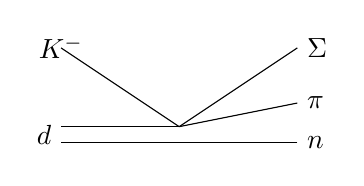
\begin{tikzpicture}
          \draw (-1.5,    1) node {$K^-$}--(0,    0);
          \draw (-1.5,    0)--(0,    0);
          \draw (-1.5, -0.2)--(0, -0.2);
          
          \node (d) at (-1.5, -0.1) [left] {$d$};
          
          \draw ( 1.5,  1.0) node [right] {$\Sigma$} -- (0,    0);
          \draw ( 1.5,  0.3) node [right] {$\pi$}    -- (0,    0);
          \draw ( 1.5, -0.2) node [right] {$n$}      -- (0, -0.2);
        \end{tikzpicture}
        \\
        (a) 1-step reaction
          
        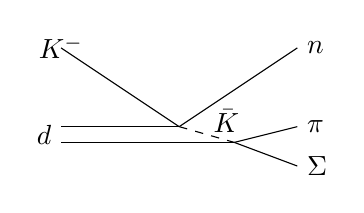
\begin{tikzpicture}
          \draw (-1.5,    1) node {$K^-$}--(0,    0);
          \draw (-1.5,    0)--(0,    0);
          \draw (-1.5, -0.2)--(0.7, -0.2);
          \node (d) at (-1.5, -0.1) [left] {$d$};
          
          \draw (0, 0) -- (0.7, -0.2) [dashed];
          \node (barK) at (0.6, -0.2) [above] {$\bar{K}$};
          
          \draw ( 1.5,  -0.5) node [right] {$\Sigma$} -- (0.7, -0.2);
          \draw ( 1.5,  -0.0) node [right] {$\pi$}    -- (0.7, -0.2);
          \draw ( 1.5,  1.0) node [right] {$n$}      -- (0,    0);
        \end{tikzpicture}
        \\
        (b) 2-step reaction
      \end{figure}
    \end{minipage}
  \end{tabular}
\end{frame}


\chapter{Experimental setup}
%% \chapter{Experimental setup}
\section{Experimental facility}
\subsection{J-PARC}

The J-PARC is located at the Tokai village in Ibaraki Prefecture.
J-PARC, which means Japan Proton Accelerator Research Complex, consists of some facilities,
which are nuclear transmutation facility, materials, and the Material Life Science Experimental Facility, Neutrino Experimental Facility, and Hadron Experimental Facility\cite{JPARC_had}.
The concept of the J-PARC is to provide various secondary beam for the above purpose.
The J-PARC has three accelerators,
first one is linac which is injector and accelerates proton beam to $400$MeV$/c$,
second is RCS (Rapid Cycling Synchrotrons) which accelerates proton beam to $3$GeV, which was provided to materials and life experimental facility and muon facility.
Next is MR (Main Ring) which accelerates proton beam to $30$GeV$/c$, which beam was extracted by two methods.
One is the fast extraction (FX) for the Neutrino Experimental Facility to produce a neutrino beam which transported to the super Kamiokande.
The other is the slow extraction (SX) for the Hadron Experimental Facility.
In this extraction, banched beam in the MR is gradually extracted as scraping.
For this purpose, the $30$GeV$/c$ proton beam was extracted about 2-second with a 5.2-second repetition cycle in the present experimental.

This continuous beam is irradiated on the primary target that is 6mm $\times$ 6mm $\times$ 66mm golden block
to generate secondary beam which includes anti-proton, pion, kaon and so on that is not naturally exist.
The secondary beam is transported to several beamlines.

The present experiment ix performed at the K1.8BR beamline, which was placed at north of the hadron facility and branced from the K1.8 beamline
which is optimized for beam whose momentum is around $1.8$GeV$/c$.


\subsection{K1.8BR beam line}
The K1.8BR beamline was planned to use low momentum kaon beam whose upper limit is 1.2 $GeV/c$.
Such kaon decays with short decay time, so beam line length should be short.
So, our beamline length was designed at about 31m by branching the K1.8 beamline.
Fig \ref{fig:K18BR} shows a schematic view of the K1.8BR beamline.

The D1 magnet accumulates secondary particles with the 6-degree aperture and the D2 magnet selects a specific momentum beam with $\pm$ 3\% momentum bite.
% From the D1 magnet to the D2 magnet accumulated secondary beam and selected specific momentum.
Intermediate focus slit (IF Slit) defined beam profile to increase the number of kaon beam while keeping good kaon and another particle ratio.
Kaon and other particles were separated by the electrostatic separator (ES1) using vertical direction statical electronic field
which uses the principle that different mass charged particles pass different trajectories by the electrical field.
The kaon beam was kicked up by the CM1 magnet, was bent in the opposite direction by ES1 and was kicked to parallel direction by the CM2 magnet.
Other particles pass through different position of vertical direction at mass slit1 (MS1), so these were intercepted by the MS1.
% Other particles pass through different virtical position at mass slit1 (MS1) which was intercepted by the MC1,
Also, the horizontal directional slit of the MS1 defines the dispersive of the beam.
The D3 magnet switched beam to the K1.8 or the K1.8BR.
After the D3 magnet, an SQDQD system is employed to focus the beam on the experimental target at FF of the K1.8BR beam line.
The first-order beam envelope calculated by the TRANSPORT code \cite{TRANSPORT} is shown in Fig \ref{fig:TRANSPORT}.

The data for the $d(K^-, p)$ has been taken in May-June in 2016 which is so-called as MR-RUN69 and the data for the $d(K^-, n)$ has been taken in Jan-Feb in 2018 which is so-called as MR-RUN78.

\begin{table}
  \caption[Parameters of the beam-line magnets.]{Parameters of the beam-line magnets. D5 field is a typical monitored value. Other field values are interpolations of measured points.}
  \centering
  \hspace{1cm}
  \begin{tabular}{llccccc}
    \hline\hline
    Element &       J-PARC  &       Gap or  &       Effective       &       Bend    &       Current &       Field at pole   \\
    &       designation     &        bore/2 (cm)    &       length (cm)     &       (deg)   &       (A)     &       (kG)    \\
    \hline
    D1      &       5C216SMIC       &       8       &       90.05   &       10      &       -369    &       -6.7444    \\
    Q1      &       NQ312MIC        &       8       &       67.84   &               &       -357    &       -3.075  \\
    Q2      &       Q416MIC &       10      &       87.04           &               &       -668    &       3.872   \\
    D2      &       8D218SMIC       &       15      &       99.65   &       15      &       -698    &       -8.7673 \\
    \hline
    IF-H    &       \multicolumn{4}{l}{Movable horizontal slit for acceptance control}              &               &               \\
    IF-V    &       \multicolumn{4}{l}{Movable vertical slit, (y$|\phi$)=0}                                 &               &               \\
    \hline
    Q3      &       Q410    &       10      &       54.72   &               &       -679    &       -4.108  \\
    O1      &       O503    &       12.5    &       15      &               &       -15     &       -0.29   \\
    Q4      &       Q410    &       10      &       54.72   &               &       -776    &       4.692   \\
    S1      &       SX504   &       12.5    &       27.6    &               &       -42     &       -0.29   \\
    CM1     &       4D604V  &       10      &       20      &       (0.856) &       348     &       1.633   \\
    ES1     &       Separator  &    10      &       600     &               &       \multicolumn{2}{c}{E=-500 kV/10 cm}     \\
    CM2     &       4D604V  &       10      &       20      &       (0.856) &       348     &       1.630   \\
    S2      &       SX504   &       12.5    &       27.6    &               &       -136    &       1.02    \\
    Q5      &       NQ510   &       12.5    &       56      &               &       -498    &       4.218   \\
    Q6      &       NQ610   &       15      &       57.2    &               &       -535    &       -4.316  \\
    \hline
    MOM     &       \multicolumn{5}{l}{Movable horizontal slit for momentum acceptance control}             &               \\
    MS1     &       \multicolumn{4}{l}{Movable vertical slit for $K$-$\pi$ separation }                                     &               &               \\
    &       \multicolumn{4}{l}{($y|\phi$)=0, ($y|y$)=0.844, ($y|\theta\phi$)=($y|\phi\delta$)=0}            &               &               \\
    \hline
    D3      &       6D330S  &       15      &       165.1   &       20      &       210     &       -7.064  \\
    S3      &       SX404   &       10      &       20      &               &       -34     &       -1.062  \\
    Q7      &       Q306    &       7.5     &       30.34   &               &       -464    &       4.026   \\
    D4      &       8D440S  &       20      &       198.9   &       60      &       -1938   &       -17.906 \\
    Q8      &       NQ408   &       10      &       46.5    &               &       -110    &       0.671   \\
    D5      &       8D240S  &       20      &       195.9   &       55      &       -1666   &       -16.437 \\
    \hline\hline
  \end{tabular}
  \label{tab:BL_magnet}
\end{table}

\begin{table}[htbp]
  \centering
  \begin{tabular}{ll}
    \hline \hline
    Primary beam momentum       & 30 GeV/c proton      \\
    Primary beam power          & 50kW \\
    Proton per spill            & $4.8 \times 10^{13}$ \\
    Repetition cycle            & 5.2 sec \\
    Spill Length                & 2 sec \\
    Spill suty factor           & 50\%  \\
    Spill extraction efficiency & 99.5 \% \\
    \hline
    Production target & Au(50~\% loss)\\
    Production angle  & 6 degrees \\
    Length (T1-FF)    & 31.3 m \\
    Momentum range    & 1.2 GeV/c max. \\
    Acceptance        & 2.0 msr$\cdot$\% ($\Delta\Omega\cdot\Delta p/p$)\\
    Momentum bite     & $\pm$ 3 \% \\
    \hline
  \end{tabular}
  \caption{
    Parameters of the K1.8BR beamline and typical operation condition
  }
  \label{tab:K18BR}
\end{table}


\begin{figure}[htbp]
  \centering
  \includegraphics[width=8cm]{pic/experiment/K18BR.eps}
  \caption{
    Schematic view of the K1.8BR beam line.
  }
  \label{fig:K18BR}
\end{figure}

\begin{figure}[htbp]
  \begin{centering}
    \includegraphics[width=8cm]{pic/experiment/optics.eps}
    \caption{
      First-order beam envelope calculated by the TRANSPORT.
    }
    \label{fig:TRANSPORT}
  \end{centering}
\end{figure}


\subsection{BHD and T0}
The beam particles are kaon is confirmed by the TOF method using beamline hodoscope detector (BHD) and time-zero counter (T0) in the offline analysis.
The T0 is located immediately downstream of the AC.
The BHD is located between the D5 and D4 magnets, approximately 7.7m upstream of T0, i.e. the flight length is 7.7m.

The T0 is a 5-segment plastic scintillation counter array 160mm (high) $\times$ 32mm (width) $\times$ 10mm (thick), with an effective area of 160mm $\times$ 160mm.
The T0 is installed rotated 45 degrees with respect to the beam direction as the beam is horizontally spread at the T0.
A counter uses the Saint-Gobain BC420 scintillator and attached readout which is 3/4 inch Hamamatsu H6612B photomultipliers to both sides of the scintillator.

The BHD is a 20-segment plastic scintillation counter array 160mm (high) $\times$ 20mm (width) $\times$ 5mm (thick), with an effective area of 200mm (horizontal) $\times$ 160mm (vertical).
A counter uses the same photomultipliers as the T0 counter.
The BHD is installed at the most upstream of the beamline and the number of beams per spill is a few M ($\times 10^6$)events,
so the photomultipliers are attached high voltage booster to the last three dynodes to avoid gain drop due to high current by high rate beam.

\subsection{Beam line chamger}
\begin{figure}[htbp]
  \centering
  \begin{tabular}{ccc}
    \begin{minipage}{0.33\hsize}
      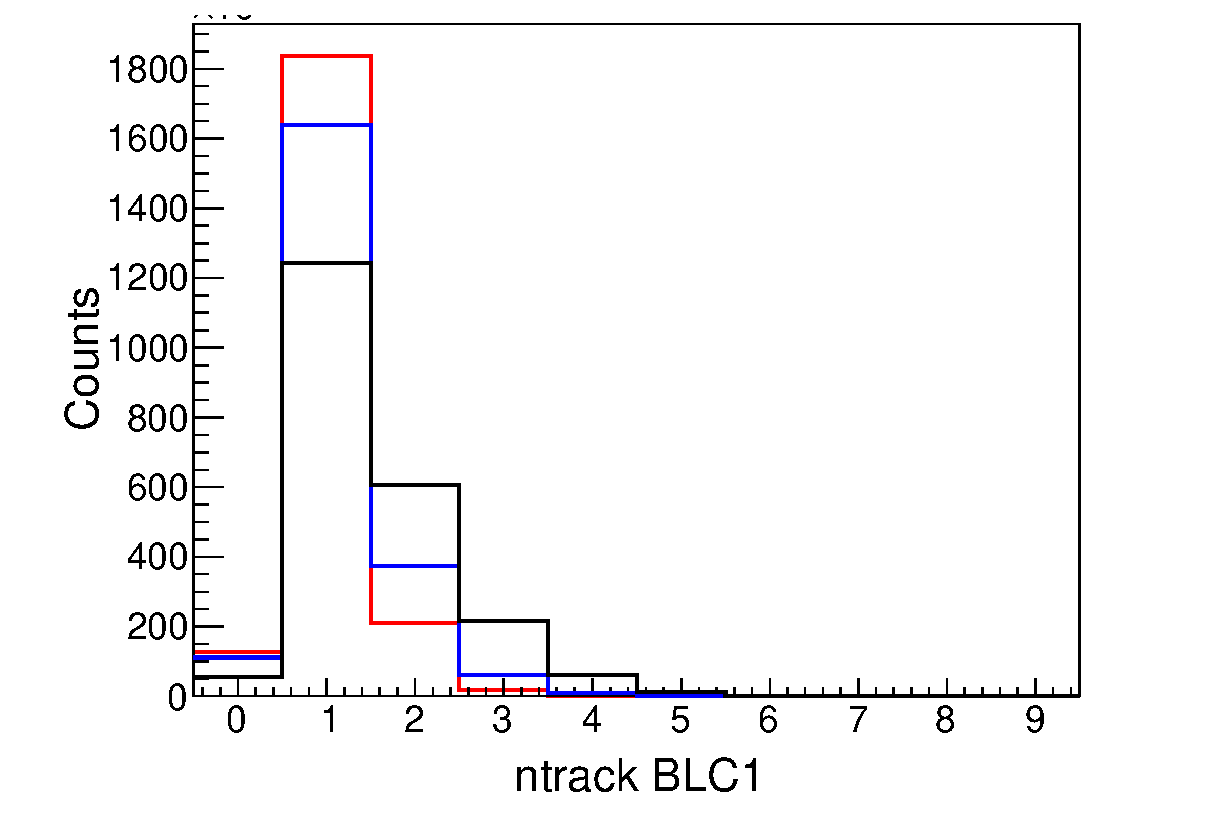
\includegraphics[width=4cm]{../pic/Run78/BL/nBLC1.eps}
    \end{minipage}
    \begin{minipage}{0.33\hsize}
      \includegraphics[width=4cm]{../pic/Run78/BL/BLC1_time.eps}
    \end{minipage}
    \begin{minipage}{0.33\hsize}
      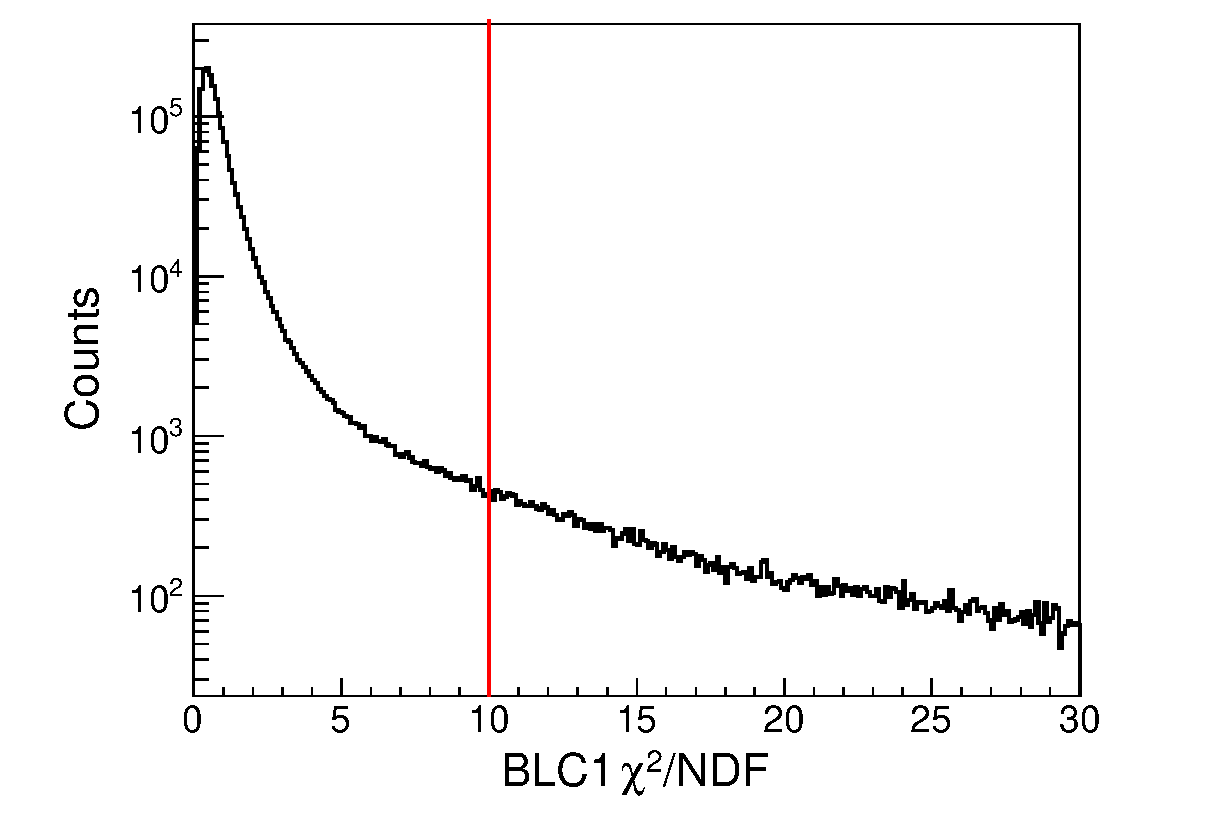
\includegraphics[width=4cm]{../pic/Run78/BL/BLC1_chi2.eps}
    \end{minipage}
  \end{tabular}
  
  \begin{tabular}{ccc}
    \begin{minipage}{0.33\hsize}
      \includegraphics[width=4cm]{../pic/Run78/BL/nBLC2.eps}
    \end{minipage}
    \begin{minipage}{0.33\hsize}
      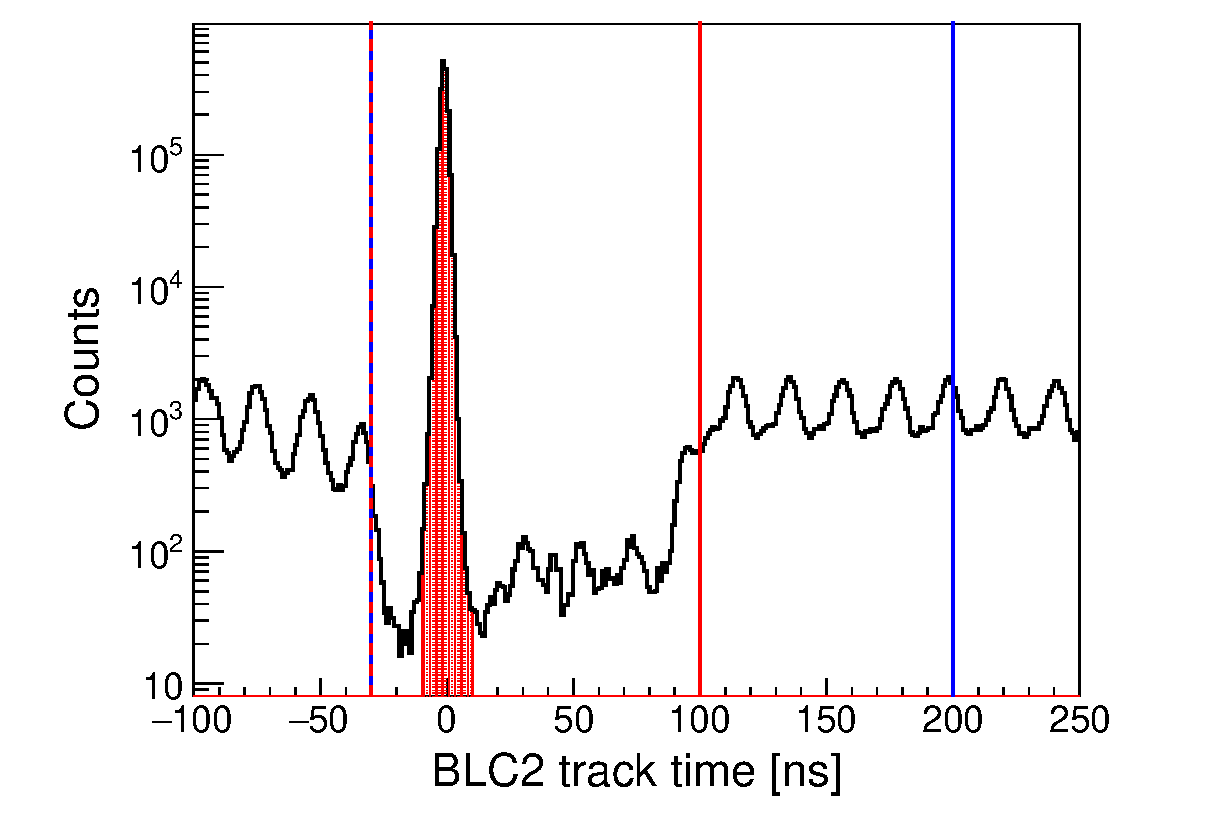
\includegraphics[width=4cm]{../pic/Run78/BL/BLC2_time.eps}
    \end{minipage}
    \begin{minipage}{0.33\hsize}
      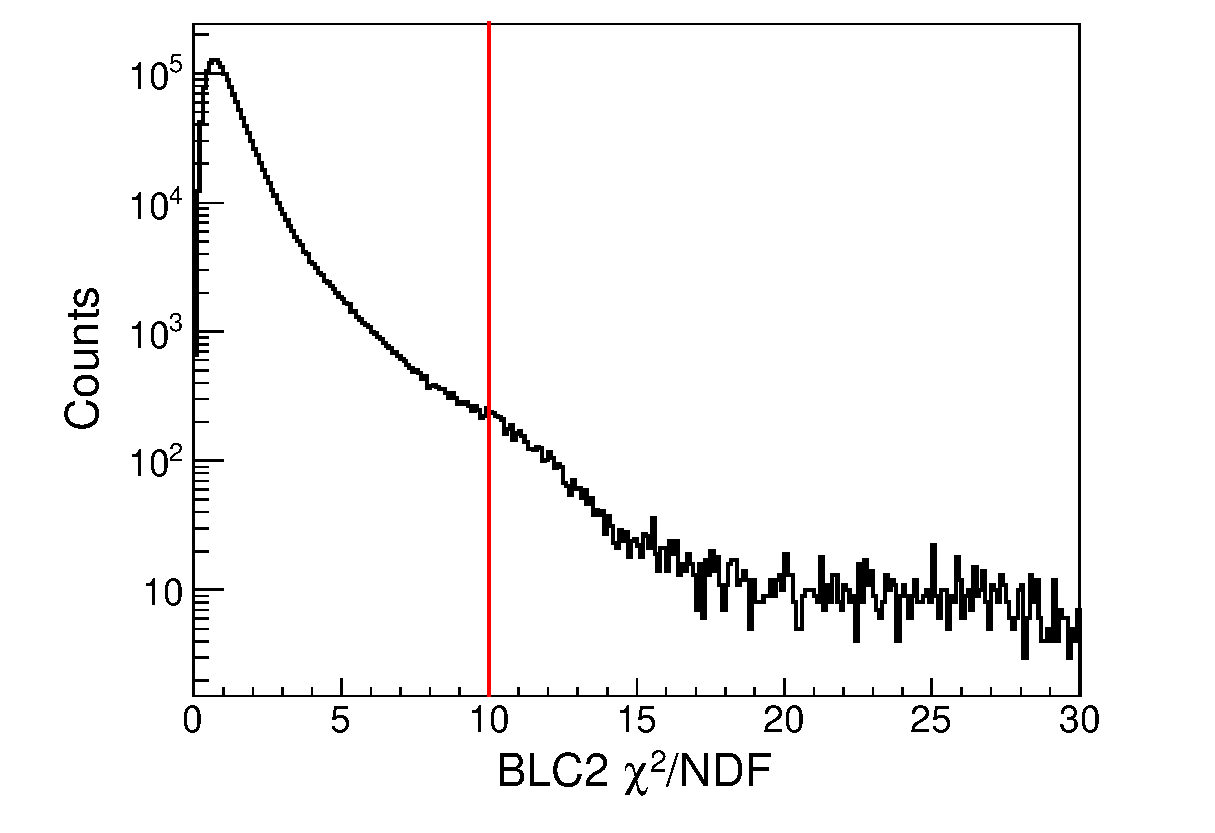
\includegraphics[width=4cm]{../pic/Run78/BL/BLC2_chi2.eps}
    \end{minipage}
  \end{tabular}
  
  \begin{tabular}{ccc}
    \begin{minipage}{0.33\hsize}
      \includegraphics[width=4cm]{../pic/Run78/BL/nBPC.eps}
    \end{minipage}
    \begin{minipage}{0.33\hsize}
      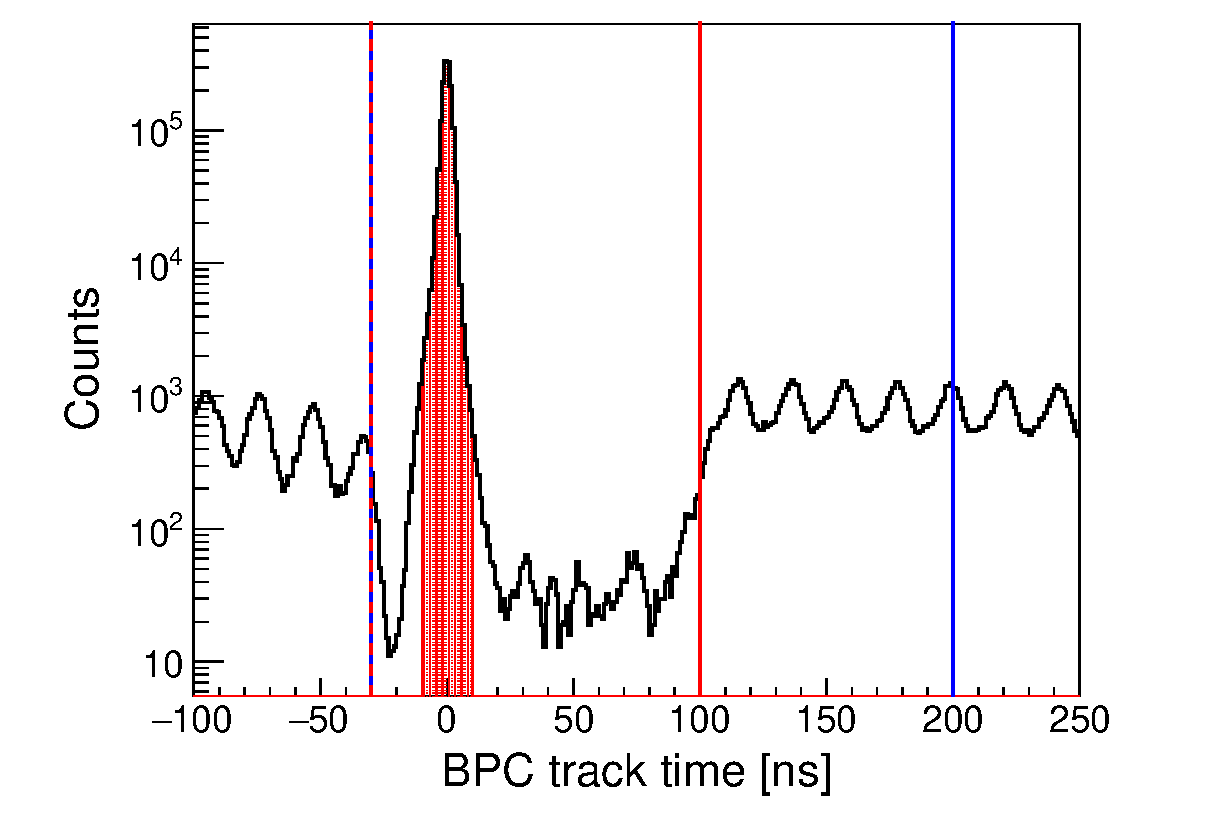
\includegraphics[width=4cm]{../pic/Run78/BL/BPC_time.eps}
    \end{minipage}
    \begin{minipage}{0.33\hsize}
      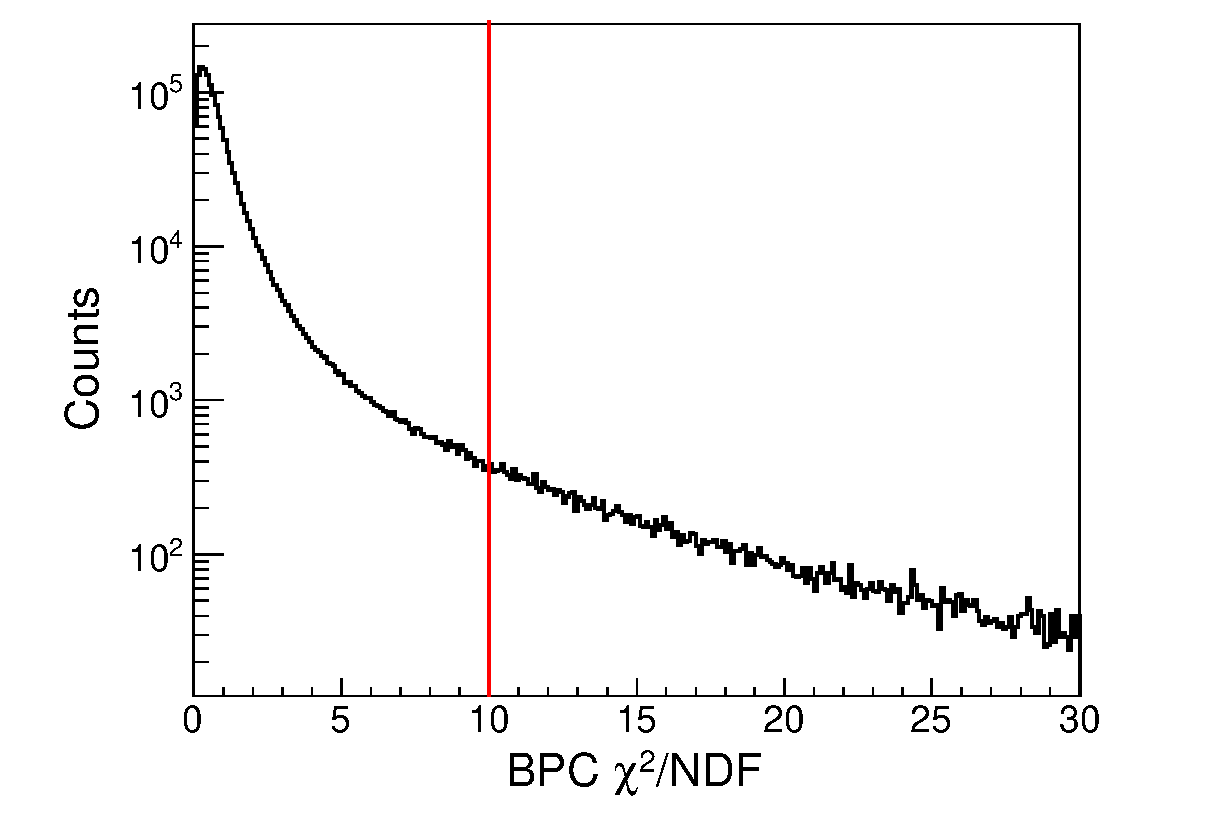
\includegraphics[width=4cm]{../pic/Run78/BL/BPC_chi2.eps}
    \end{minipage}
  \end{tabular}
  \caption{
    The left, the middle and the right figures show the number of tracks, track time and $\chi/NDF$, respectively.
    Color plots in the left figure indicate some time window.
    % Black, blue, red indicate all, $-30\sim200$[ns], $-30\sim100$[ns], respectively.
    The above, the middle and the down figures represent BLC1, BLC2 and BPC, respectively.
    The BPC was described after.
  }
  \label{fig:BLC_etc}
\end{figure}
BLC1 and BLC2 were installed upstream and downstream of the D5 magnet, respectively to measure beam momentum using the transfer matrix of the D5 magnet.
These are planer the type drift chamber whose drift length was calculated using the X-T map, which was the integration of drift time.
The track time of BLC was estimated from timing signals of pair plane due to constant drift length.
SX beam has RF-structure seems like the center figures of Fig\ref{fig:BLC_etc}, so we select synchronization about beam which indicates the red hatched region.
The left figures represent the number of tracks, in which black, blue, and red indicate time window of all, $-30\sim100$[ns], and $-30\sim200$[ns], respectively.
We select 1track events in red time window selection to keep statistics.
The right figures show $\chi^2/NDF$ distribution after 1track selection.
We accepted $\chi^2/NDF<10$ events as good track.

\subsection{BPC analysis}
\subsection{BLC2-BPC matching}
\begin{figure}[htpb]
  \centering
  \begin{tabular}{cc}
    \begin{minipage}{0.5\hsize}
      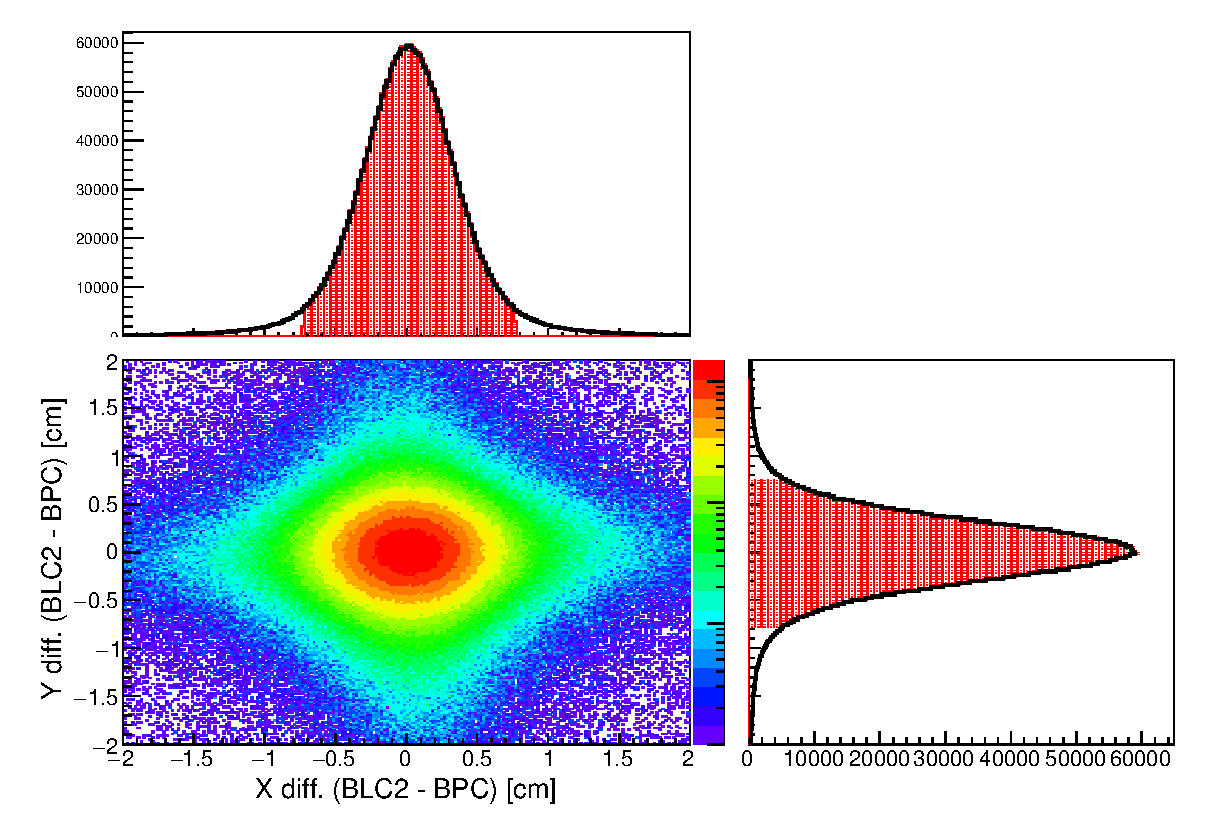
\includegraphics[width=6cm]{../pic/Run78/BL/BLC2BPC.eps}
    \end{minipage}
    \begin{minipage}{0.5\hsize}
      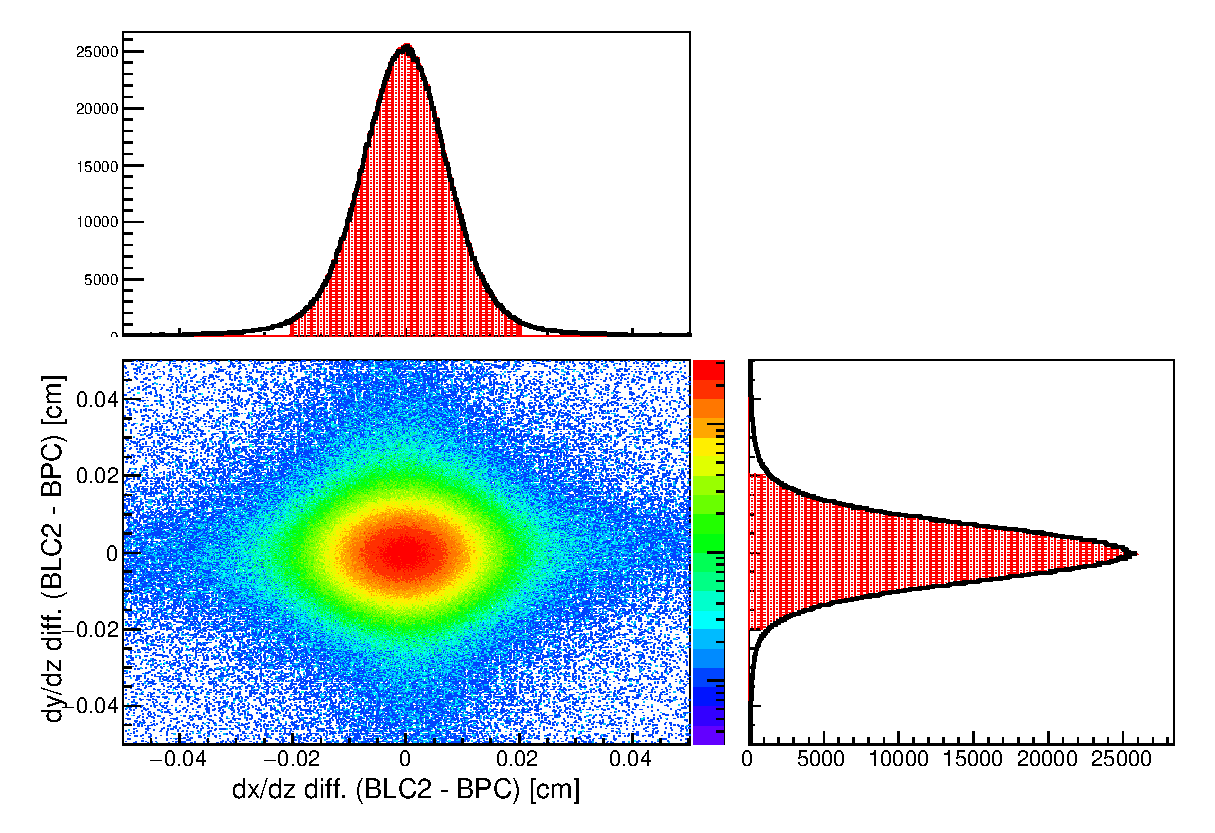
\includegraphics[width=6cm]{../pic/Run78/BL/BLC2BPC_dir.eps}
    \end{minipage}
  \end{tabular}
  \caption{
    These figures indicate the connection between the BLC2 and the BPC.
    The left figure shows about position matching at the center of these.
    The right figure shows direction matching.
    The red hatched region indicated an acceptable region.
  }
  \label{fig:BLC2BPC}
\end{figure}

\begin{figure}[htpb]
  \begin{tabular}{cc}
    \begin{minipage}{0.5\hsize}
      \includegraphics[width=6cm]{../pic/Run78/BL/profFF_Kf.eps}
    \end{minipage}
    \begin{minipage}{0.5\hsize}
      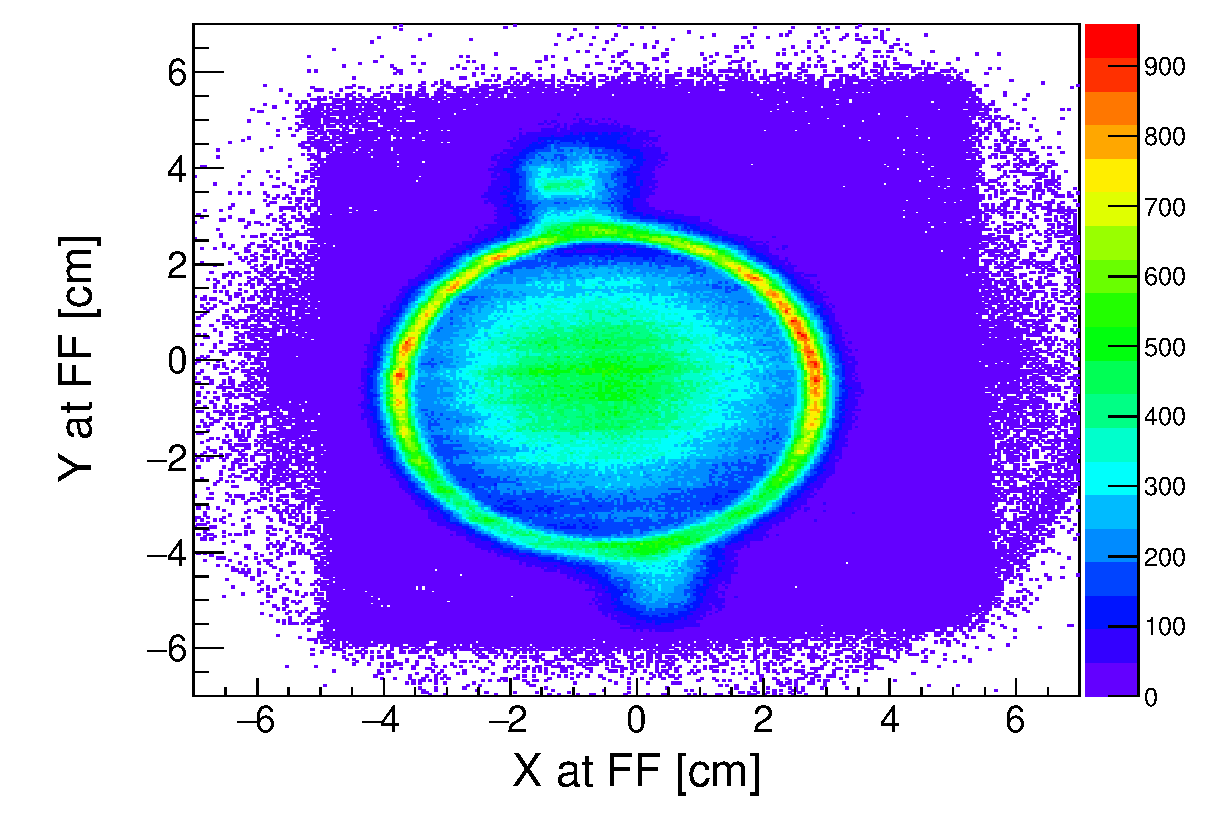
\includegraphics[width=6cm]{../pic/Run78/BL/profFF_KCDH2.eps}
    \end{minipage}
  \end{tabular}
  \caption{
    These figures shows beam profile at FF.
    The left figure shows about the unbiased kaon trigger.
    The right figure shows about CDH2 hit trigger.
  }
  \label{fig:profFF}
\end{figure}
The BPC is the same type drift chamber as BLC1/2, so the analysis of itself is the same as BLC1/2, which is shown in Fig\ref{fig:BLC_etc}.
There is no magnet between the BLC2 and the BPC, so trajectories reconstructed by them sshould be successfully connected within multiple scattering and resolution.
There are many materials between the BLC2 and the BPC, for example, the T0, the AC, BPD, and air, also direction ($dx/dz$ or $dy/dz$) resolution affects on extracted position resolution.
The $z$ length ratio of these is (BPC $z$)/(BLC2 $z$)=50.4mm/310mm$\sim$1/6, so extracted position resolution was almost decided by the BPC.
On the other hand, materials were placed at just down stream of the BLC2 for example the T0 and the AC.
These two effects were estimated almost the same, so we evaluated position matching at the center of the BLC2 and the BPC as Fig\ref{fig:BLC2BPC}.
We also require direction matching the right figure of Fig\ref{fig:BLC2BPC}.
The BPC also defines The beam profile at the experimental target position as shown in Fig\ref{fig:profFF}.
The profile required reaction at the trigger level was clearly seen target cell.
The red circle indicates an acceptable region as an effective kaon beam. %% todo Fiducialの赤枠

\begin{figure}[htpb]
  \begin{tabular}{cc}
    \begin{minipage}{0.5\hsize}
      \includegraphics[width=6cm]{../pic/Run78/BL/profFF_Kf.eps}
    \end{minipage}
    \begin{minipage}{0.5\hsize}
      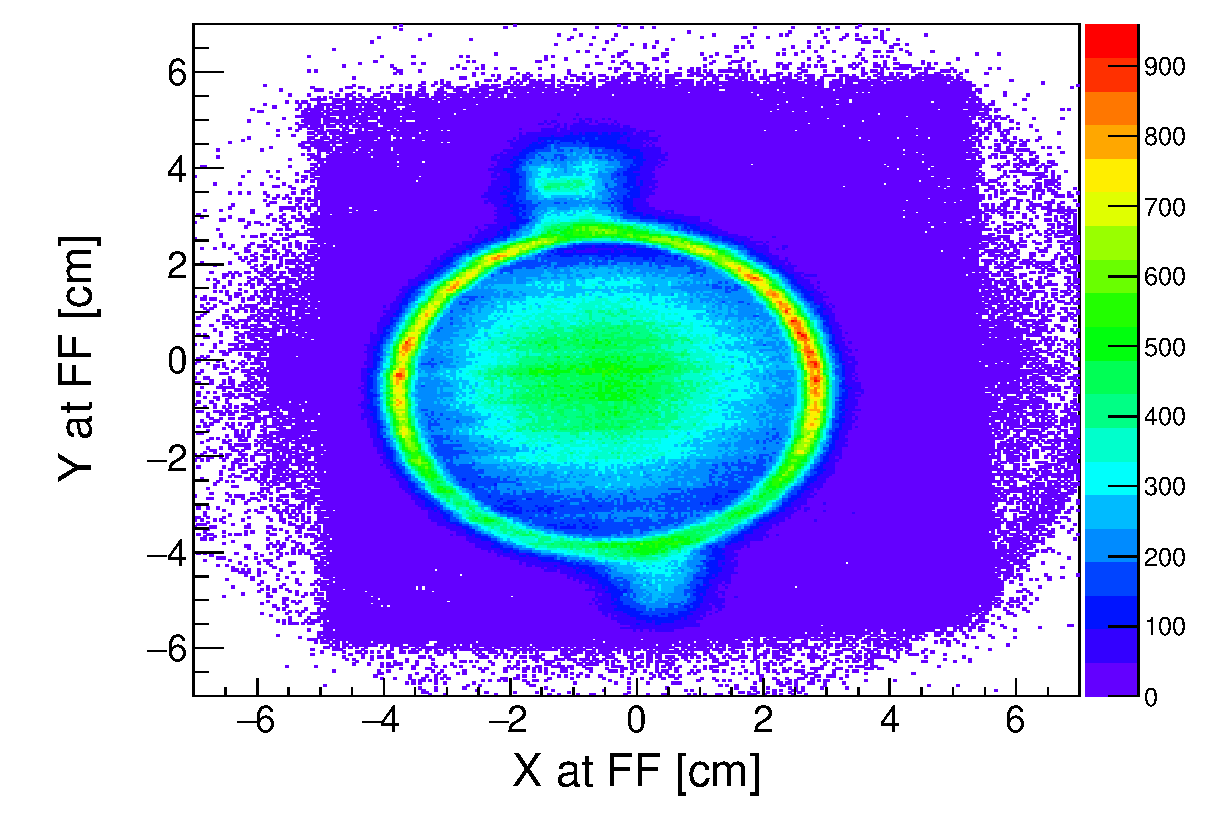
\includegraphics[width=6cm]{../pic/Run78/BL/profFF_KCDH2.eps}
    \end{minipage}
  \end{tabular}
  \caption{
    These figures shows beam profile at FF.
    The left figure shows about the unbiased kaon trigger.
    The right figure shows about CDH2 hit trigger.
  }
  \label{fig:beam_prof_fFF}
\end{figure}


The BPC 1track is selected according to the conditions of Sec.\ref{sec:BLC}.
BLC2 and BPC require those tracks to match because there is no magnet between them.
They are shown in Fig.\ref{fig:BLC2BPC}
The left figure shows the difference in position between BLC2 and BPC in the center position and the right figure shows the difference in inclination of the tracks.
A $3\sigma$ acceptance region is set for each horizontal and vertical position and inclination, all of which are accepted as the correct beam.
The acceptance regions are indicated the read hatched in thr figure.

Fig.\ref{fig:beam_prof_FF} shows the beam profile from the BPC at the centre of the liquid deuterium target.
The left figure shows one from the unbaised kaon trigger and the right figure shows one from the CDH2 trigger, which requires that the beam has reacted with the material.
Fiducial volume accepted as the Kaon beam passed through indicated the red circle.

\subsection{Beam Definition Counter - DEF}
Beam definition counter (DEF) is mounted to the target vacumm chamber to define beam which pass through near the liquid-$D_2$ target.
The DEF is a 3mm plastic scintillator because it is placed just upstream of the liquid-$D_2$ target and multiple scattering and energy loss need to be reduced.

In our beamline, a half of kaon hits the liquid-$D_2$ target due to large beam size.
Kaon which do not hit the target increases trigger signal  for DAQ, which reduce DAQ efficiency.
The DEF signal is used to be coincided with beam trigger coincided from the T0 signal and the BHD signal  and successfully reduce the number of trigger signal about 30\%.


\section{Target system} \label{sec:target}
\subsection{Luquid $D_2$ target system}

\begin{figure}[htbp]
  \centering
  \includegraphics[width=10cm]{pic/experiment/d2-cryo.eps}
  \caption{
    Schematic drawing of the liquid $D_2$ cryostat.
  }
  \label{fig:d2_cryo}
\end{figure}


A side view of the cryostat for the liquid $D_2$ target is shown in Fig\ref{fig:d2_cryo}.
Deuterium is stored 1000$l$ in a tank as gases which is room temperature and 2atm keeping positive pressure after liquefaction for avoiding contamination from other materials.
The $D_2$ gas is fed into the cryostat through the top flange.
Cooling of $D_2$ is performed by the Gifford–McMahon (G–M) refrigerator (Sumitomo Heavy Industries, Ltd., RDK-145D and CSA-71A) built into the cryostat.
The cooling is performed by 2-step.
The cooling power at the first and second stages is 35$W$ at 50K and 1.5$W$ at 4.2K, respectively.
A copper plate is anchored to the first-stage cold head of the G-M refrigerator in inlet pipe for the pre-cooling of the $D_2$.
Another inlet pipe is directly connected through the top flange to the head exchanger for measuring the pressure of the $D_2$ target inside of the heat exchanger.
Since this pipe has a larger conductance, a safety valve that prevents a sudden pressure rise is also connected to it.
The $D_2$ gas is cooled in the heat exchanger where the second stage of the G–M refrigerator is thermally contacted.

\begin{figure}[htbp]
  \begin{tabular}{cc}
    \begin{minipage}{0.7\hsize}
      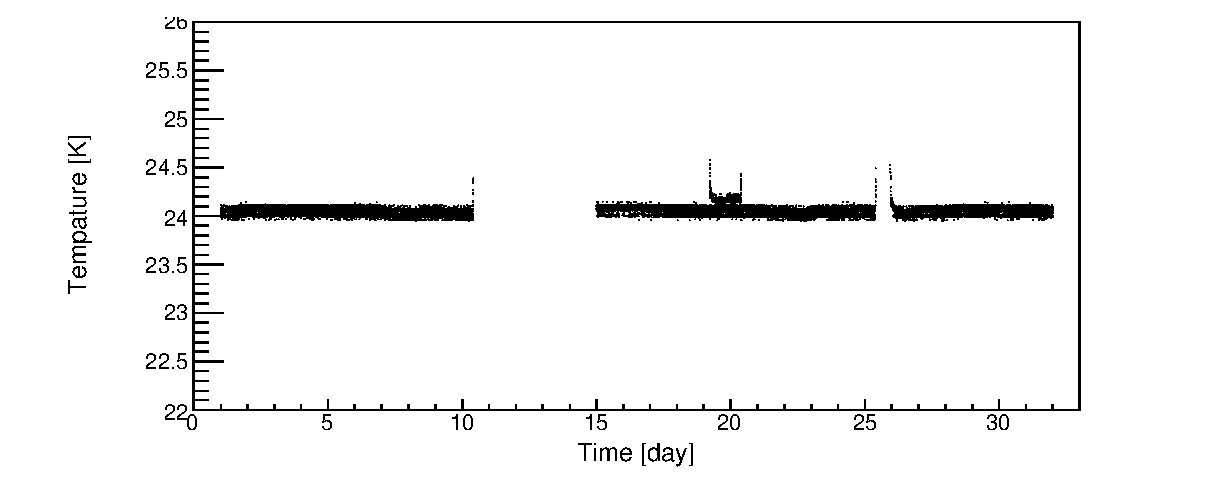
\includegraphics[width=8cm]{../pic/Dron/target/target_temp.eps}
    \end{minipage}
    \begin{minipage}{0.3\hsize}
      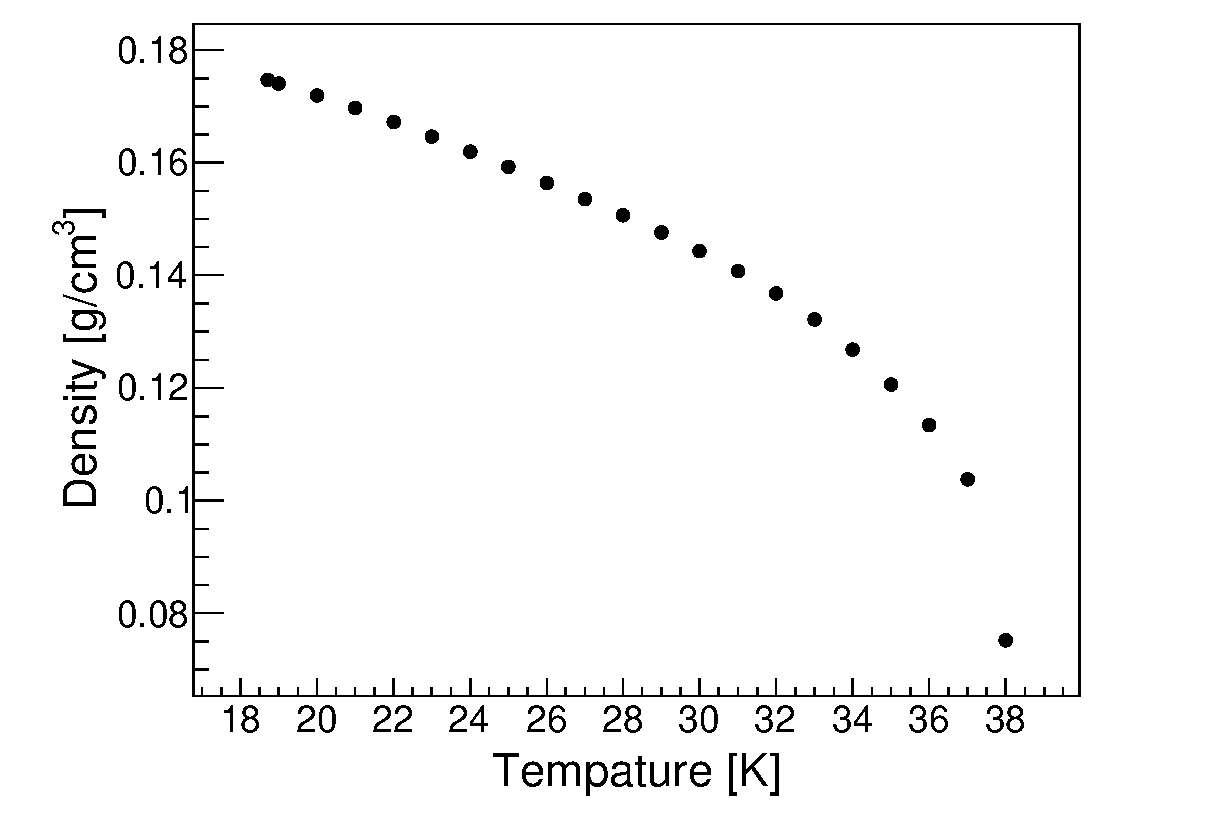
\includegraphics[width=5cm]{../pic/Dron/target/target_den.eps}
    \end{minipage}
  \end{tabular}
  \caption{
    The left figure shows the temperature of the $D_2$ target.
    The right figure shows the relation of the density and the $D_2$ temperature at 1 atm.
  }
  \label{fig:target}
\end{figure}


The target cell is $6.8cm$ diameter and $12.5cm$ length cylinder made of PET.
Liquifregrated $D_2$ is transferred by downpipe and warmed liquid $D_2$ by the heat load is returned through the upper pipe,
so the heat is effectively transferred between the target cell and the heat exchanger\cite{Target}.
Since the temperature range of liquid $D_2$ is narrow as 18.7-23.8K at 1 atm, the temperature of the $D_2$ should be controlled in the liquid range to avoid blocking due to the solid $D_2$.
Since the cooling power of the second stage of the G–M refrigerator is larger than the heat load on the low-temperature parts,
The current in the heater is controlled by a proportional-integral-derivative (PID) algorithm with an input of the temperature of the heat exchanger.
Target cell temperature in MR-RUN78 is represented in Fig\ref{fig:target} which is monitored by Pt-Co thermometer (CHINO R800-6) whose tolerance was $\pm$ 0.5K.
The same figure also shows the relation of temperature and density of $D_2$ at 1 bar.
The error of $D_2$ density was estimated at 1.5$\times 10^{-3} [g/cm^3]$ from tolerance and fluctuation.


\begin{frame}{CDC fine turning}
  \begin{tabular}{cc}
    \begin{minipage}{0.5\hsize}
      \begin{figure}
        Before\\
        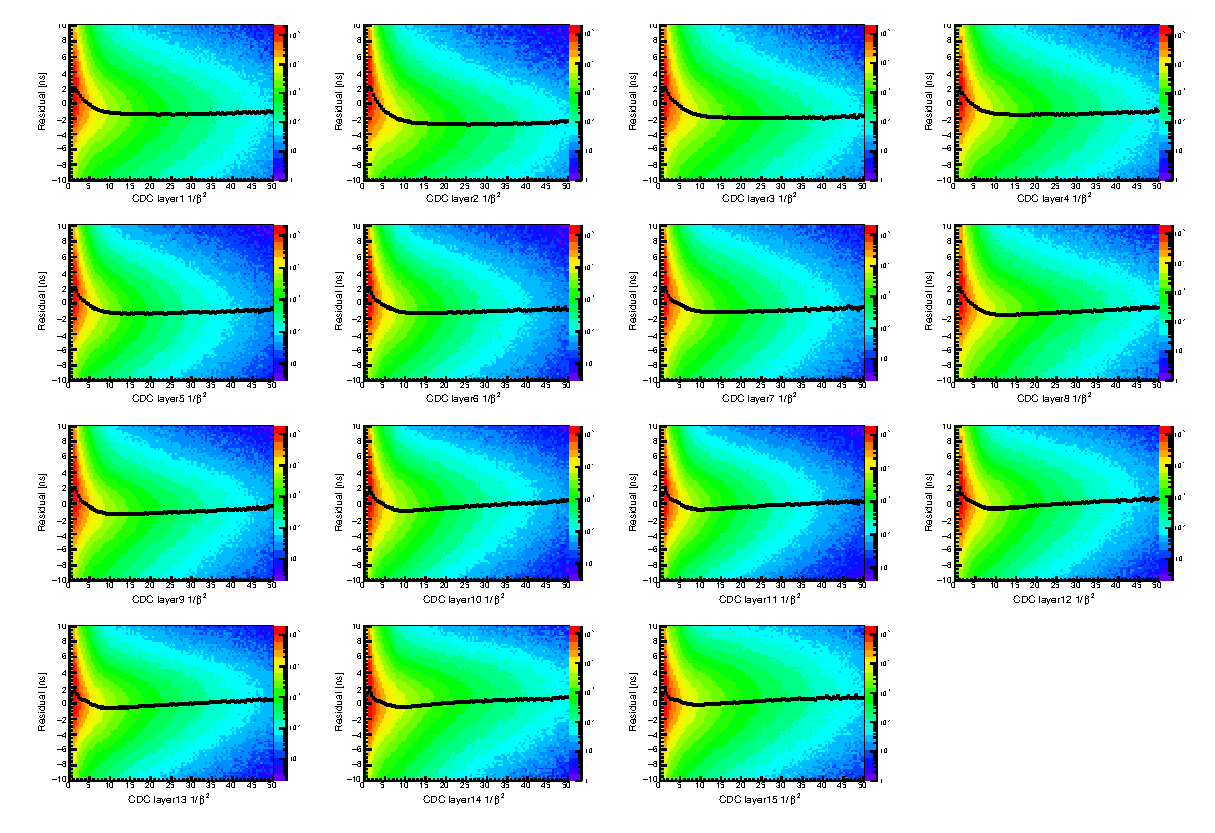
\includegraphics[width=5cm]{../pic/Run78/CDS/CDC_ob2_res_before.eps}
      \end{figure}
    \end{minipage}

    \begin{minipage}{0.5\hsize}
      \begin{figure}
        After\\
        \includegraphics[width=5cm]{../pic/Run78/CDS/CDC_ob2_res.eps}
      \end{figure}
    \end{minipage}
  \end{tabular}
  \centering
  $\beta$ and residual has correlation, which was calibrated wire-by-wire.
\end{frame}

\begin{frame}{Vertex image by CDS and BPC}
  \begin{figure}
    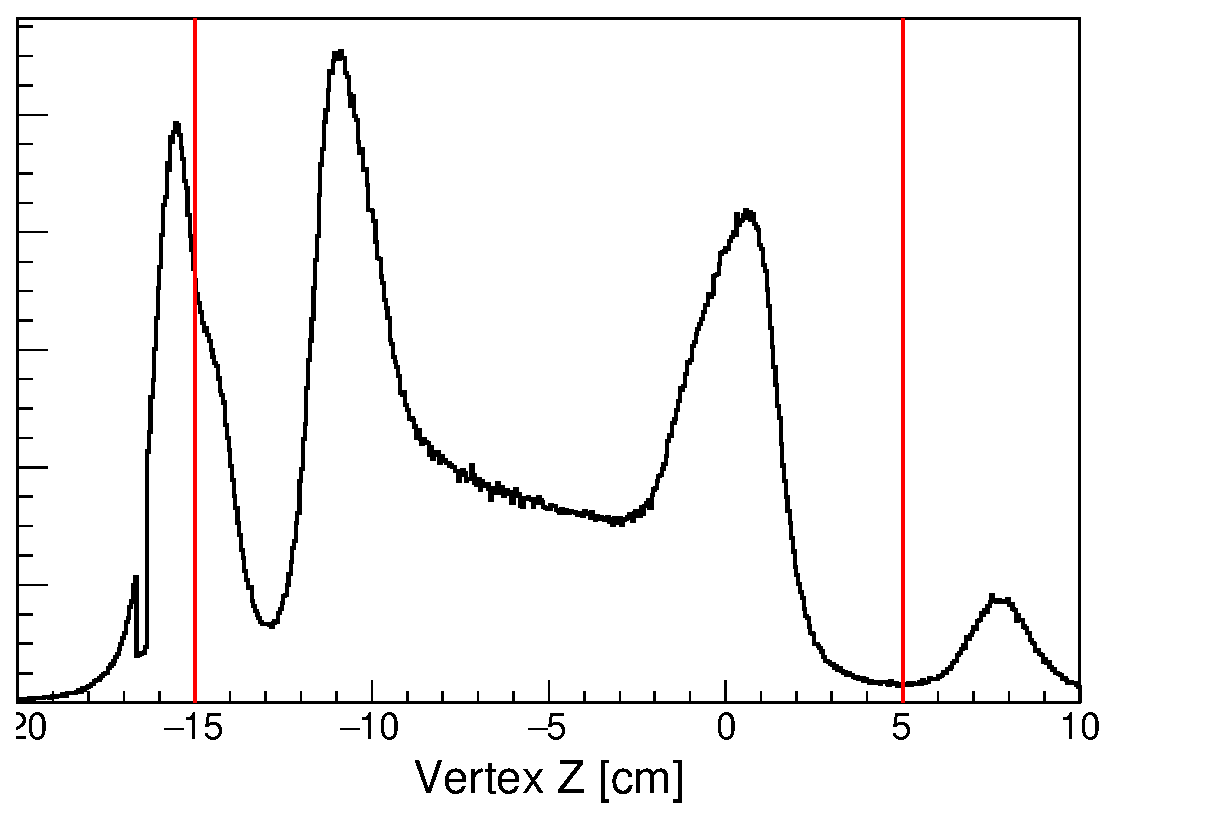
\includegraphics[width=8cm]{../pic/Run78/CDS/vertex.eps}
  \end{figure}
\end{frame}

\begin{frame}{Vertex image by CDS and BPC (Vertex cut)}
  \begin{figure}
    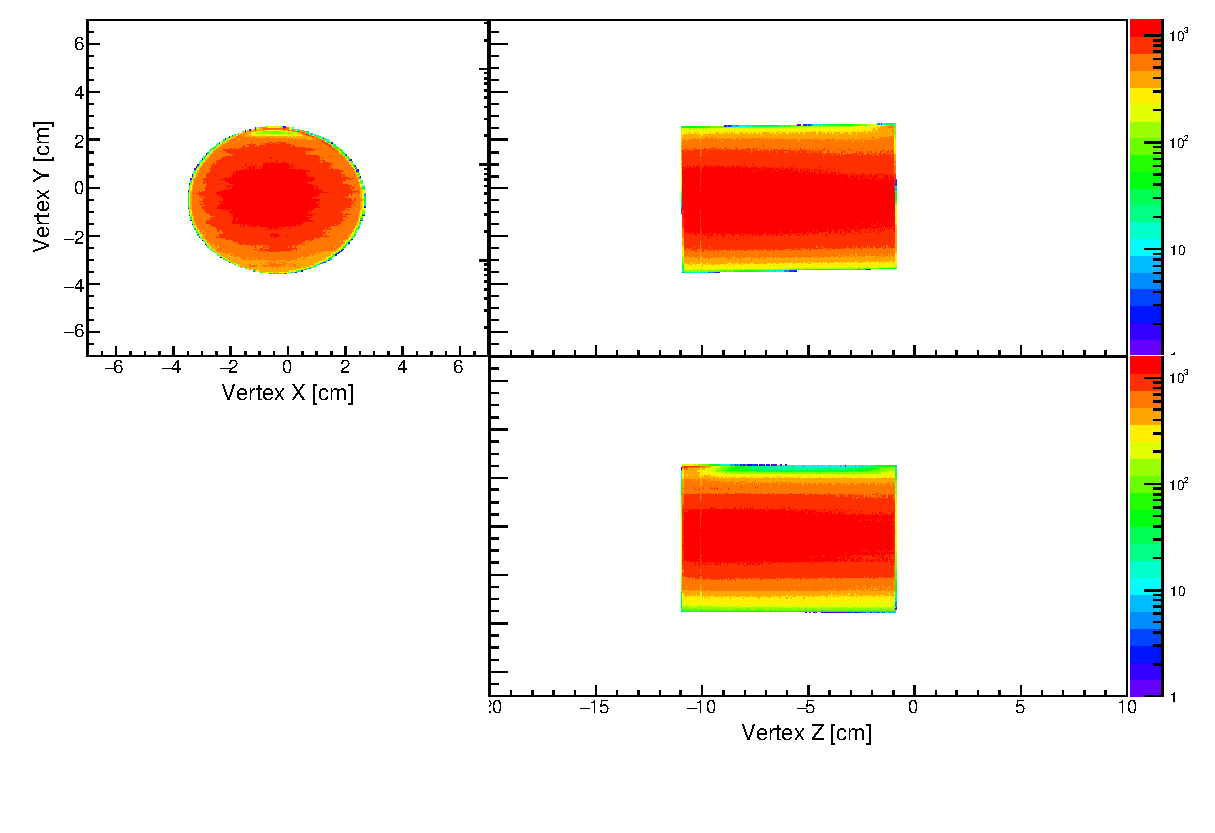
\includegraphics[width=8cm]{../pic/Run78/CDS/vertex_f.eps}
  \end{figure}
\end{frame}

\begin{frame}{Vertex resolution}
  \begin{tabular}{cc}
    \begin{minipage}{0.5\hsize}
      \begin{figure}
        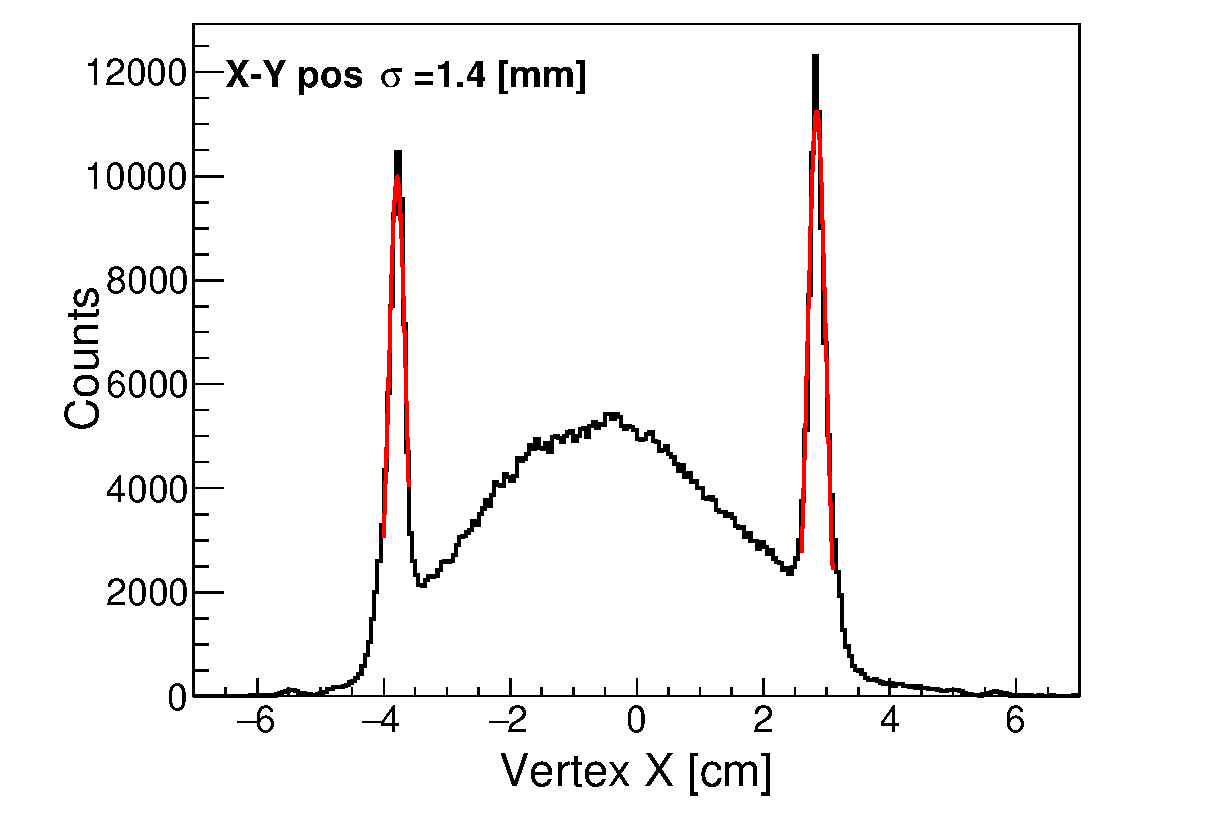
\includegraphics[width=5cm]{../pic/Run78/CDS/vertex_x.eps}
      \end{figure}
      \centering
      Y range was selected \\ $-5.5\sim-5$ [mm]
    \end{minipage}

    \begin{minipage}{0.5\hsize}
      \begin{figure}
        \includegraphics[width=5cm]{../pic/Run78/CDS/vertex_z.eps}
      \end{figure}
      \centering
      $Z =0$ was selected [mm]\\
      resolution was evaluated by DEF.
    \end{minipage}
  \end{tabular}
\end{frame}

\begin{frame}{CDS mass$^2$ vs momentum}
  \begin{figure}
    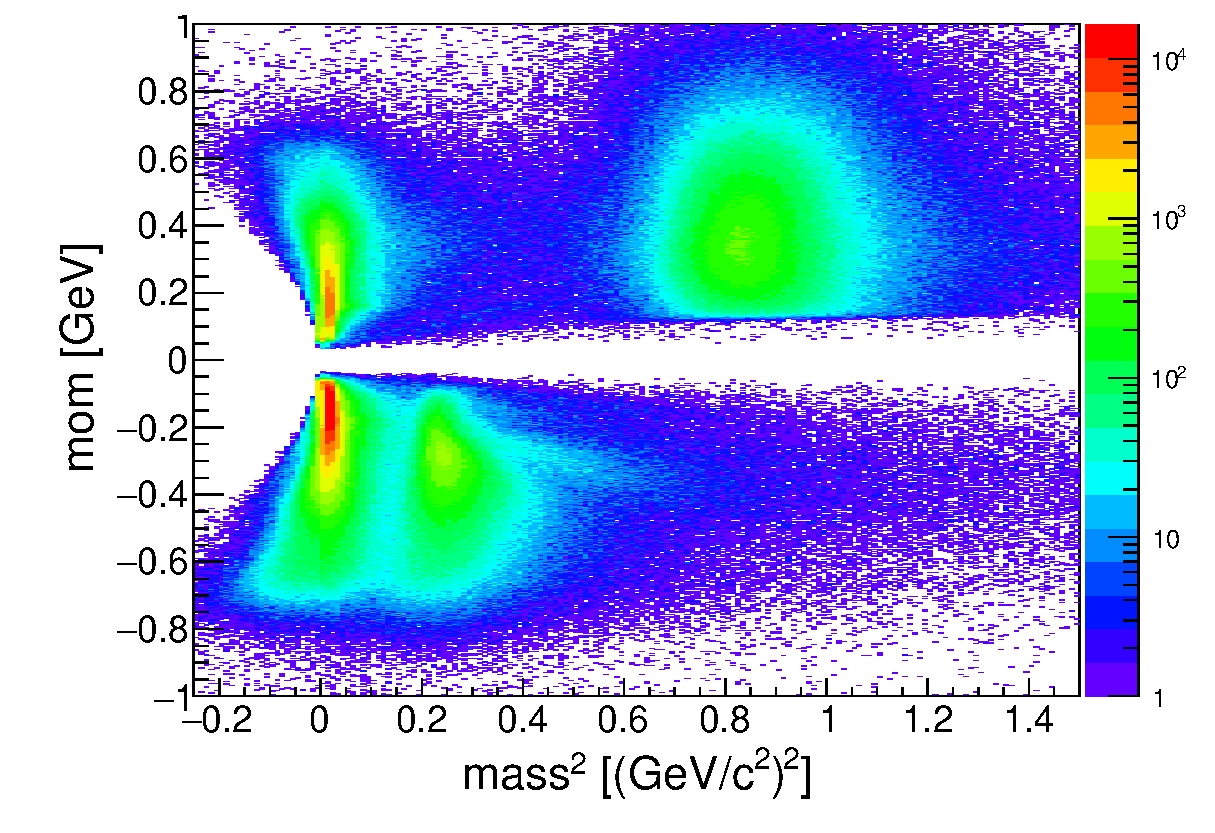
\includegraphics[width=8cm]{../pic/Run78/CDS/pid.eps}
  \end{figure}
\end{frame}

\begin{frame}{Invaraint mass by CDS}
  \begin{tabular}{cc}
    \begin{minipage}{0.5\hsize}
      \begin{figure}
        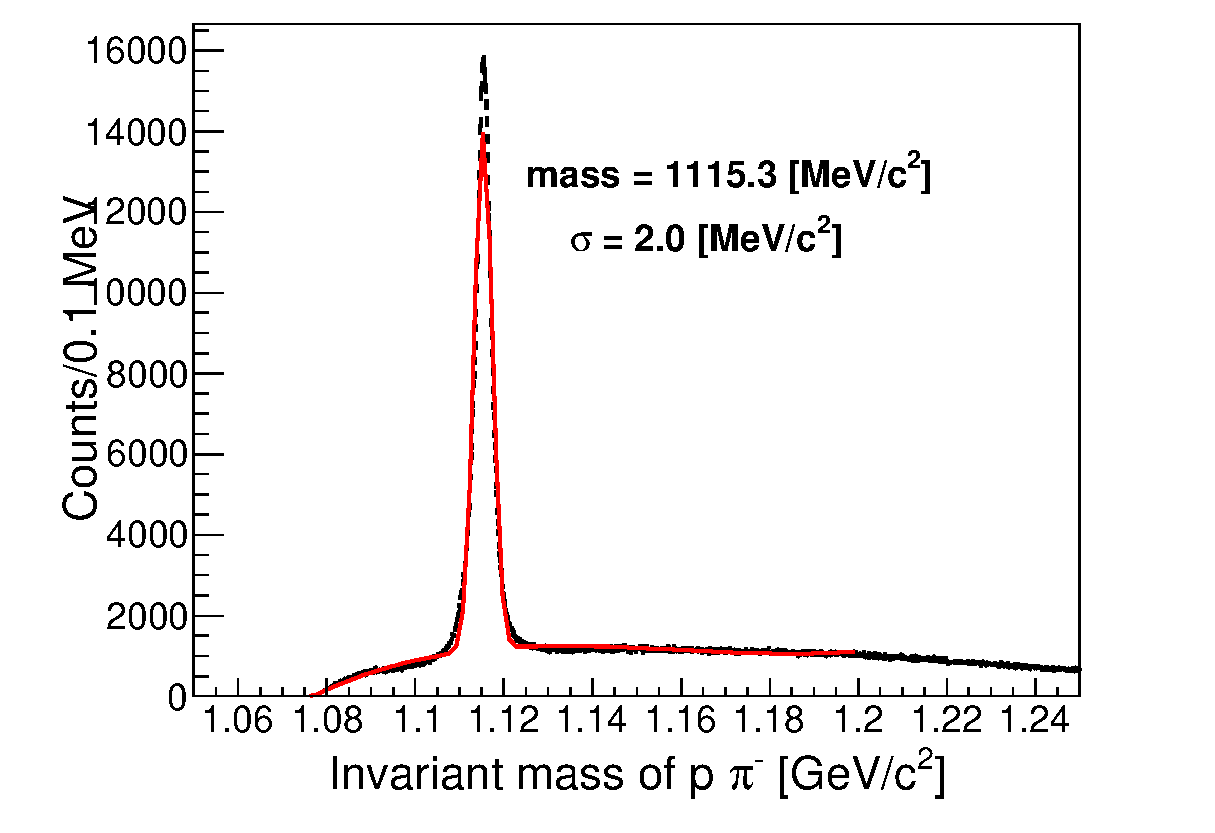
\includegraphics[width=5cm]{../pic/Run78/CDS/IM_ppim.eps}
      \end{figure}
    \end{minipage}

    \begin{minipage}{0.5\hsize}
      \begin{figure}
        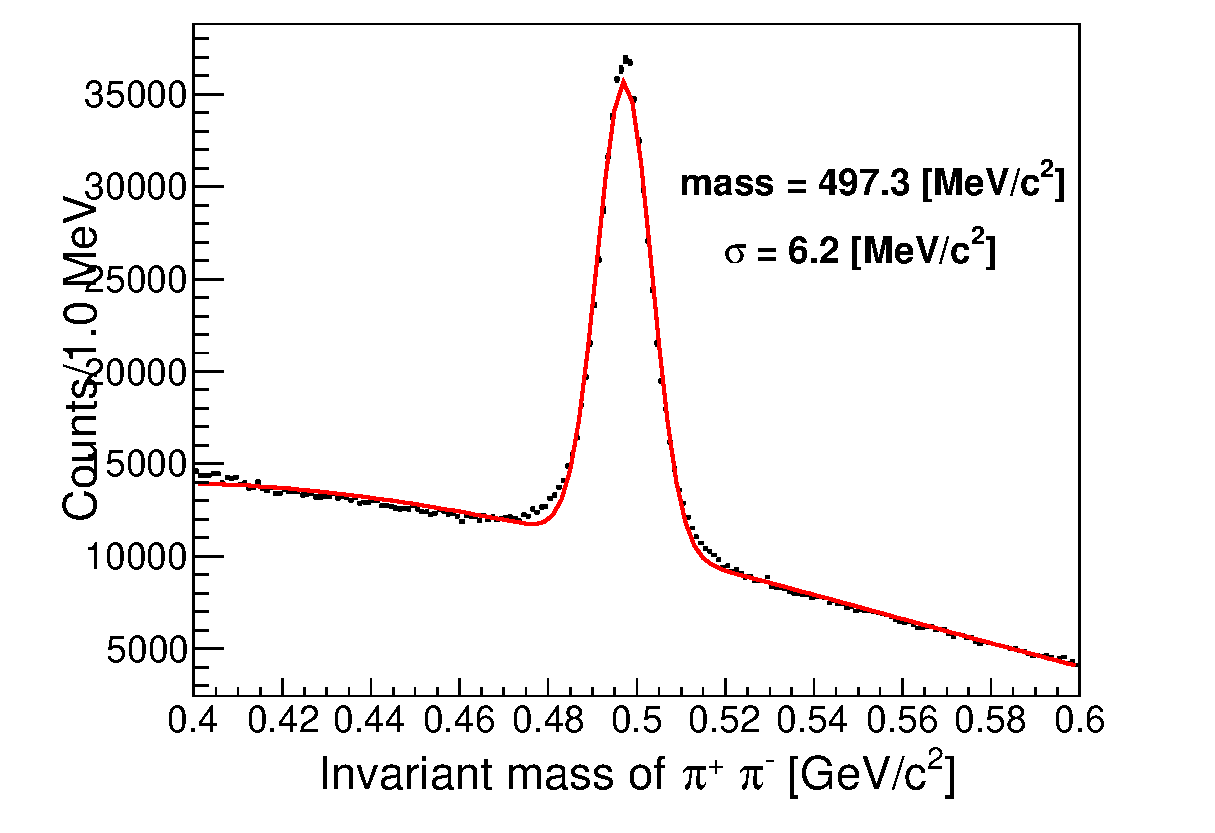
\includegraphics[width=5cm]{../pic/Run78/CDS/IM_pipi.eps}
      \end{figure}
    \end{minipage}
  \end{tabular}
\end{frame}



\begin{figure}[htbp]
  \centering
  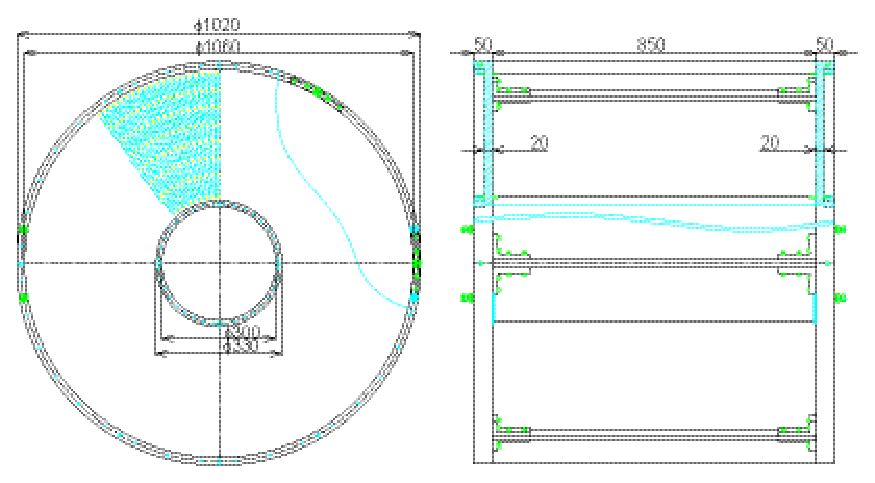
\includegraphics[width=10cm]{pic/experiment/CDC_structure.eps}
  \caption{
    Design of the CDC (all dimensions in mm).
    The CDC consists of two aluminum end-plates, a 1mm thick CFRP cylinder as an inner wall, and six aluminum posts that are placed outside the tracking volume.
  }
  \label{fig:CDC_structure}
\end{figure}

\subsection{Cylindrical Detector Hodoscope - CDH}
The CDH is a segmented plastic scintillation counter used for the charged particle trigger and particle identification.
The CDH is located at a radius of 544mm from the beam axis covering a polar angle range from 54 to 126 degree corresponding to a solid angle coverage of 59$\%$ of 4$\pi$.

The CDH consists of 36 modules, individually mounted on the inner wall of the solenoid magnet.
The scintillators are mode of ELJEN EJ-200, with dimensions of 790mm in length, 99mm in width, and 30mm in thickness.
The scintillation light is transferred through light guides to a pair of Hamamatsu R7761 fine-mesh 19-dynode photomultipliers 1.5 inches in diameter.

The CDH is operated in the 0.7T magnetic field with a typical PMT gain of $\sim 10^6$.
The measured average time resolution of the CDH without a magnetic field is $71\pm3$ ps ($\sigma$), obtained with cosmic ray data. The error represents the variation among the segments.



\section{Forward detector systems}
Beam pass through the target was swept to the beam dump direction by the beam sweep magnet called Ushiwaka,
which also used to sweep positive charged particles to the opposite direction of the beam.\\
The neutron counter array (NC) was placed at about 15m downstream of the target to detect neutral particles and measure its velocity by TOF method.
The charged particle was rejected by the beam veto counter (BVC) and the charged veto counter (CVC),
which was installed at just upstream of the Ushiwaka and the NC, respectively.
The proton counter was located at the opposite position of the beam dump to measure positive charged particles.\\
Half of the CVC was also used for a positive charged particle.
Because the trajectory of the charged particle depends on its momentum, the forward drift chamber was installed at upstream of the Ushiwaka magnet to decide its trajectory.
The momentum of forward positive charged particle was evaluated by the TOF method.

\subsection{Beam sweeping magnet}
The Ushiwaka placed at 250cm downstream of the target has a large aperture which of 82cm (horizontal) $\times$ 40cm (vertical) and a pole length of 70cm, which is larger than the acceptance of the NC.
The Ushiwaka can be applied to 1.6T at maximum value.

\subsection{Beam veto counter}
\begin{figure}[htbp]
  \centering
  \includegraphics[width=10cm]{pic/experiment/BVC.eps}
  \caption{
    Schematic view of the BVC.
  }
  \label{fig:BVC}
\end{figure}
The BVC was attached on the downstream flange of the target cryostat to reject charged particle contamination to neutral trigger, especially come from beam particle pass through.
The coverage size of the BVC is 320mm (height) $\times$ 320mm (width) $\times$ 10mm (thickness) made of ELJEN EJ-200. This size is large enough to cover the acceptance of the neutron counter.
The BVC is horizontally segmented int 8units with different sizes as shown in Fig\ref{fig:BVC} to avoid the over-concentration to the beam on the central segments.
In this position, there is some leak magnetic field from the solenoid magent of the CDS and the Ushiwaka magnet so its read-out used 1-inch fine-mesh Hamamatsu R5505 photomultipliers
which were attached on both ends of each scintillator segment through Lucite light guides.


\subsection{Neutron Counter - NC}
The neutron counter (NC) are located 14.7 m upstream of the target.
Because the NC are located at the most upstream and the purpose is to detecting neutral particles, the NC requires a large amount of material.
Therefore, the NC is a segmented scintillation detector with 7 layers, each layer consisting of 16 counters.
One scintillation detector is 20cm (width) $\times$ 150cm (height) $\times$ 5cm (thickness) in size.
So one layer covers 320cm (width) $\times$ 150cm (height), which is corresponds 6.2 degrees in horizontal and 2.9 degrees in vertical in this experiment setup.
The first three layers of the scintillator are made of Saint-Gobain BC408 and the other four layers are made of Saint-Gobain BC412.
The scintillation light is carried by lucite light guides on both sides and read out by the 2-inch PMT (Hamamatsu H6410).
Each layer is installed with a gap of 2 cm, so the whole NC has a thickness of 47 cm.
Differences between the upstream and downstream solid angles are evaluated as systematic errors.

\subsection{Charge Veto Counter - CVC}
The charge veto counter (CVC) is installed just upstream of the NC to confirm that particles detected by the NC is actually neutral.
Half of the CVC is used to detect the proton.
The CVC consists of 34 segmented plastic scintillators whose size is 10cm (width) $\times$ 150cm (height) $\times$ 5cm (thickness).
A 2-inch Hamamatsu Photomultipliyer H6410 is attached to each side of the scintillator through a Lucite light guide.
The scintillator is of Eljen EJ-200 type. The average time resolution measured with cosmic rays is 78 $\pm$ 7 ps ($\sigma$).
The error represents the variation among the segments.

\subsection{Proton Counter - PC}
The proton detector (PC) is a hodoscope array for detecting positive charged particles located immediately next to the CVC in the direction opposite to the beam dump.
The PC is a 27-segmented detector using scintillators of the same size as the CVC, i.e. it has an effective area of 270 m (horizontal) $\times$ 150 m (vertical).
% However, charged particles are bent and their bending angle depends on their momentum, so their acceptance depends on their momentum.
The photomultipliyer of the PC is the same as the CVC, but the scintillator is a Saint-Gobian BC408.
The average time resolution measured with cosmic rays is 75 $\pm$ 6 ps ($\sigma$),  i.e. the time resolution does not differ from the CVC


\subsection{Forward drift chamber}
The forward drift chamber (FDC1) was attached to the Ushiwaka magnet to measure the trajectory of the forward proton before sweeping for the decision of flight-length.
The FDC1 is a planer type dift chamber that has 6 layers consists of UU'-XX'-VV'.
UU' and VV' layers were tilted $\pm 30 ^{\circ}$ about the beam axis.
Each layer has a 6mm gap in each sense wires and each pair plane was located at 20mm.



\input{experimental/table/Run68_78_chamber}

\begin{frame}{DAQ efficeincy}
  \begin{figure}
    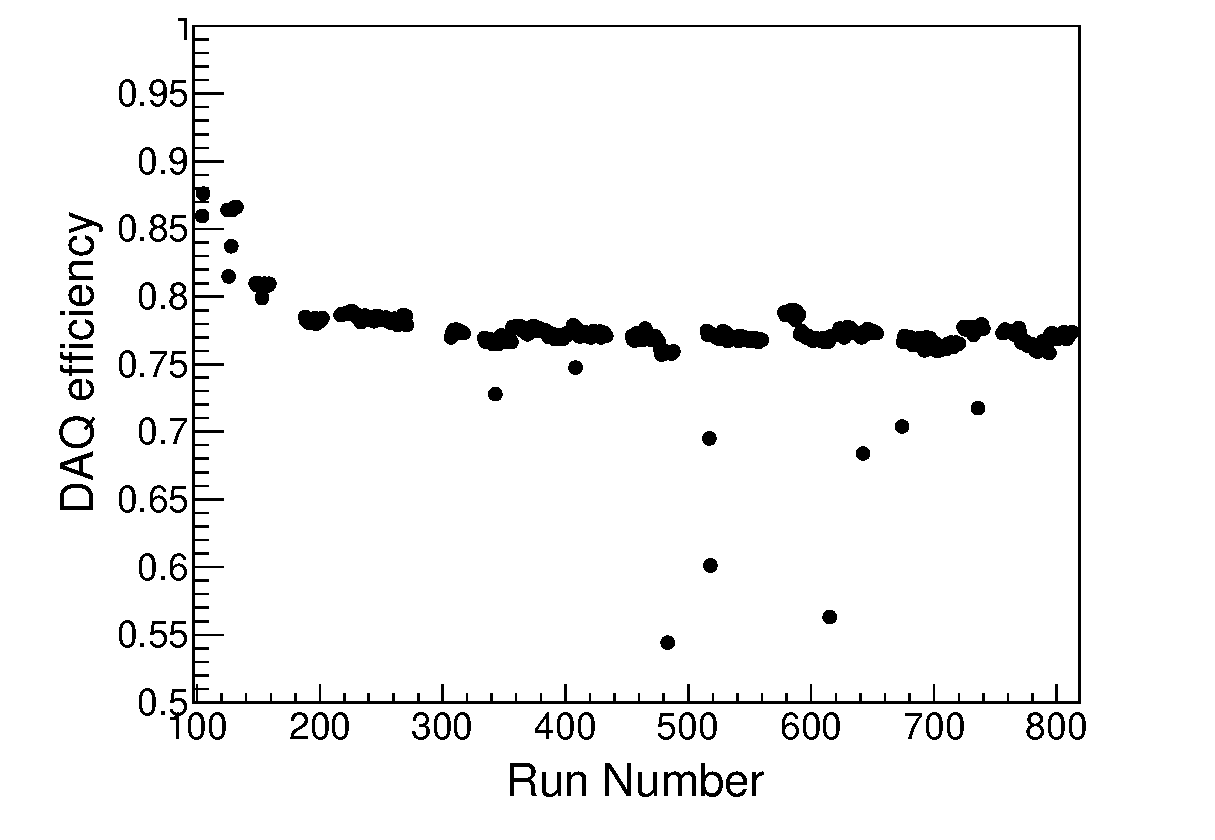
\includegraphics[width=8cm]{../pic/Run78/trigger/DAQ.eps}
  \end{figure}
\end{frame}

x% \subsection{Basical calibration}

\begin{figure}[htbp]
\begin{tabular}{cc}
\begin{minipage}{0.5\hsize}
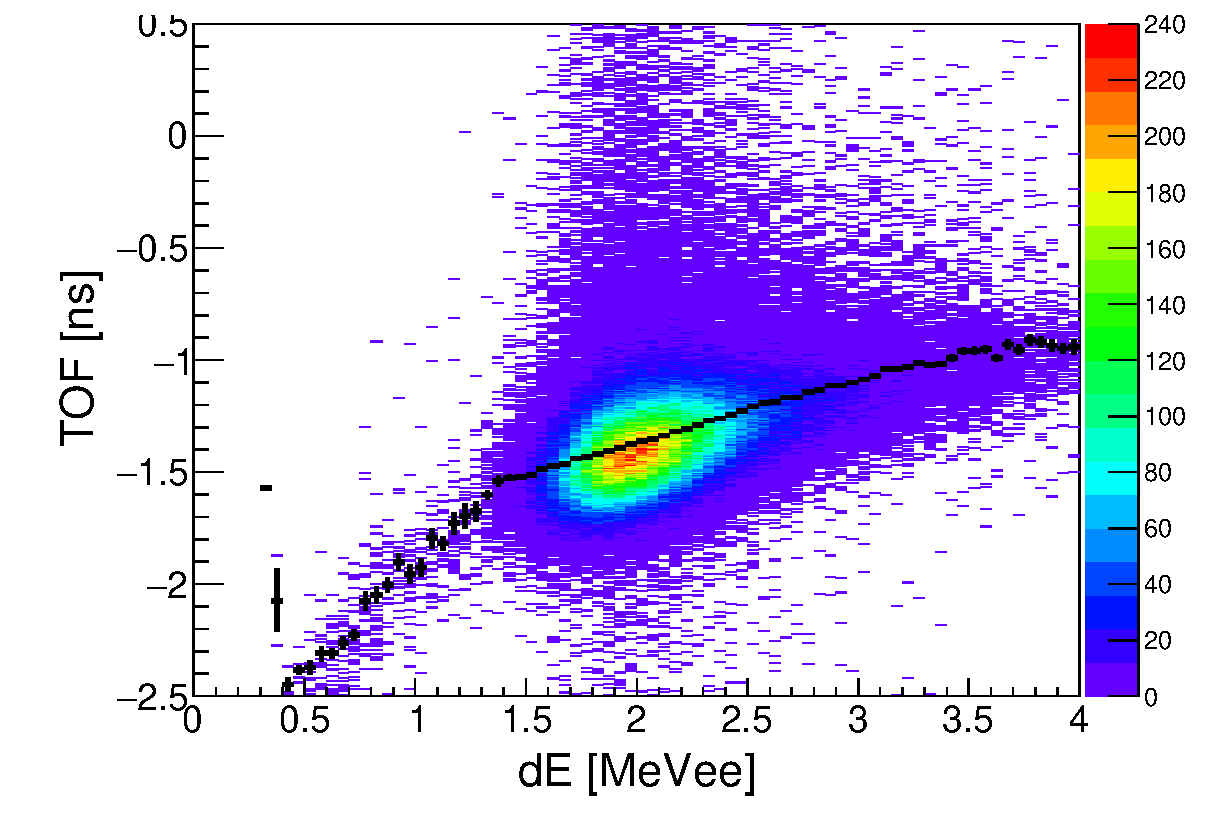
\includegraphics[width=5cm]{../pic/Dron/T0_slew_before.eps}
\end{minipage}
\begin{minipage}{0.5\hsize}
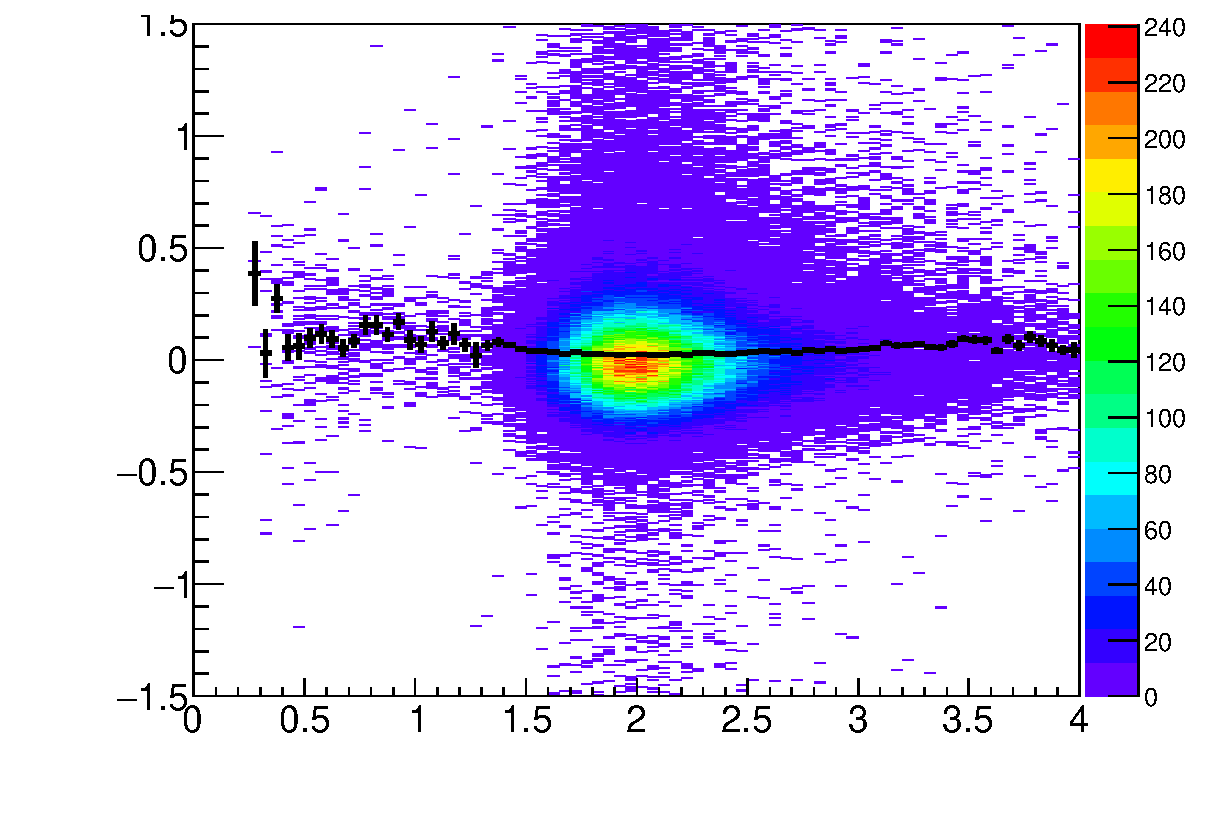
\includegraphics[width=5cm]{../pic/Dron/T0_slew_after.eps}
\end{minipage}
\end{tabular}
\caption{
  These figures indicate about slewing effect correction.
  These figures show the energy deposit of the T0 as the horizontal axis and the calculated time shift of T0-NC by the γ-ray as the vertical axis.
  The left figure shows about before correction, and the right figure shows about after correction. 
}
\label{fig:Slew}
\end{figure}

Hodoscope signals were read out as ADC and TDC data and chambers were read out only TDC. 
TDC data was converted to time.
The parameters for this were calibrated using time calibrator.
That module outputs two signals with a time difference of a certain constant multiple of time.

Hodscope had a correlation between ADC and time as shown in the left of Figure.\ref{fig:Slew} due to the rising edge of the signal.
The correlation was corrected as shown on the right of Figure.\ref{fig:Slew} by the follow function.

\begin{equation*}
  t_{corrected}=p_0+p_1 \frac{t}{\sqrt{dE}}+p_2 t
\end{equation*}

This collection was performed using a well-known timing signal.
For example, the Fig\ref{fig:Slew} shows the correction of the T0 using the $\gamma$--ray peak of the T0-NC TOF which has constant velocity.
This peak is also shown in Fig\ref{fig:NC_offset}.

Timing data of drift chambers was used to convert to the drift length.
The above figure of Fig\ref{fig:BLDC} shows the drift time distribution of the drift chamber installed at the beamline.
The middle figure indicates differentiated distribution which was used to decision start timing of each channel.
The bottom figure indicates integrated distribution which corresponds to conversion map from the drift time and the drift length by assumption that beam was uniformly irradiated on.

\begin{figure}[htbp]
\centering
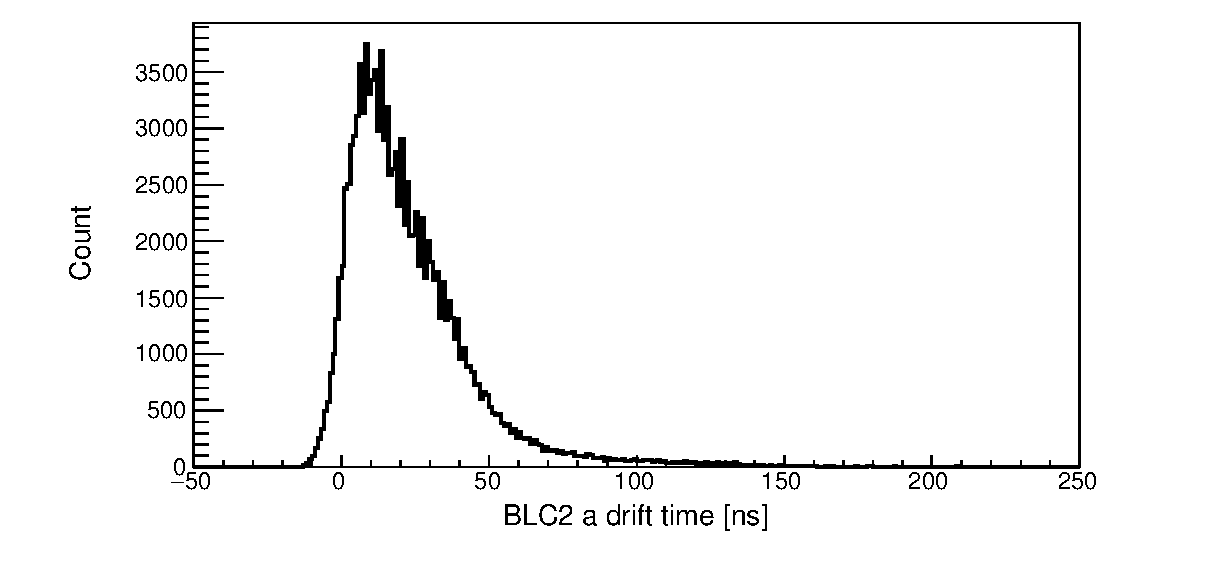
\includegraphics[width=10cm]{../pic/Dron/BLC2a_dt.eps}
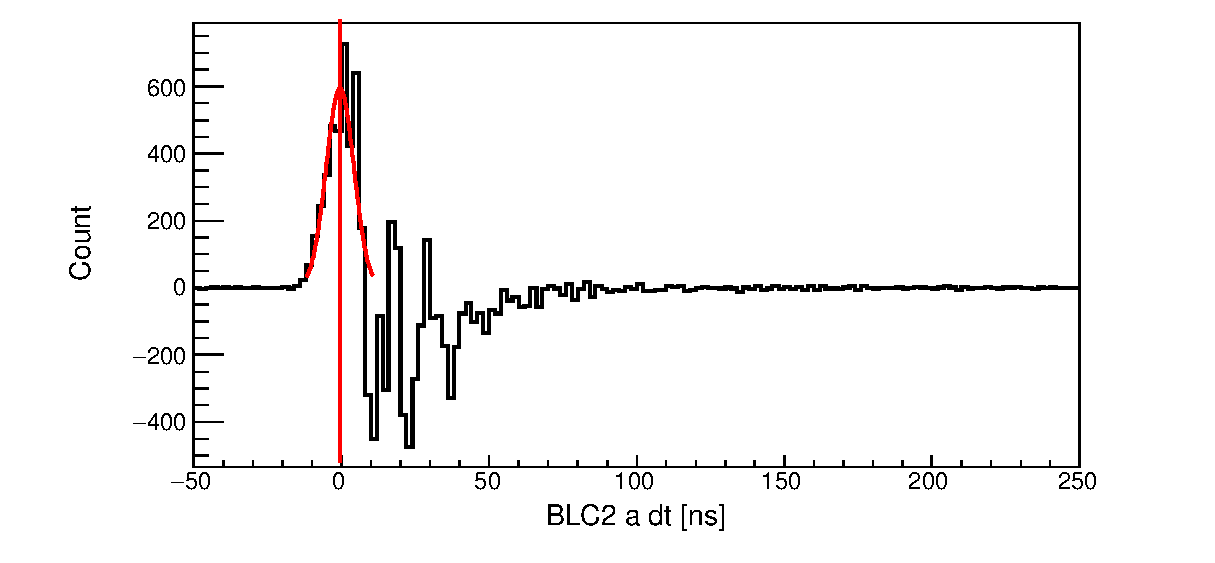
\includegraphics[width=10cm]{../pic/Dron/BLC2a_diff.eps}
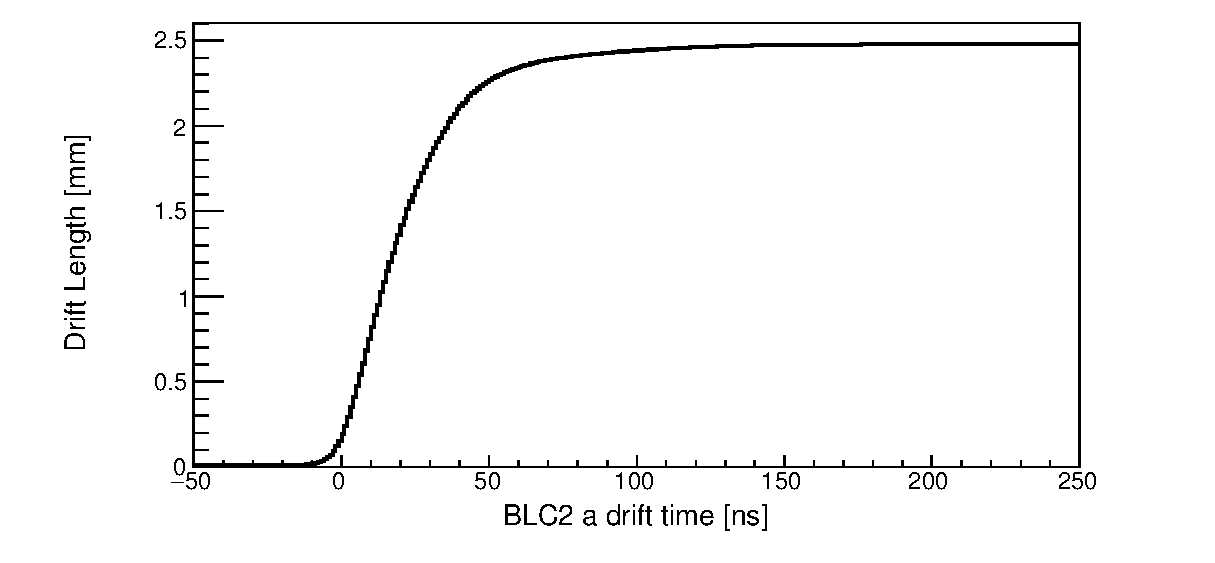
\includegraphics[width=10cm]{../pic/Dron/BLC2a_int.eps}
\caption{
  These figures indicate the calibration of drift chambers.
  The above figure shows raw distribution.
  The middle figure shows the start timing decision which is indicated by red lines.
  The bottom figure shows the $x$-$t$ map.
}
\label{fig:BLDC}
\end{figure}    




\chapter{Analysis}
%% \bibitem{helix} \href{https://www-jlc.kek.jp/subg/offl/lib/docs/helix_manip/node3.html}
                    {K. Fuji, \url{https://www-jlc.kek.jp/subg/offl/lib/docs/helix_manip/node3.html} (1968).}
\bibitem{Opera} \href{https://operafea.com/}
                {Opera Electromagnetic FEA Solution Software}
                
\bibitem{CERN_HARA_K} \href{https://cds.cern.ch/record/109658?ln=ja}
                {V. Flaminio et al., CERN-HARA-87-01, 121 (1983).}
\bibitem{KP_MB} \href{https://www.sciencedirect.com/science/article/pii/0550321375906525}
                {M.Jones et el, Nucl. Phys. B {\bf 90}, 349 (1975)}

\bibitem{tempfit} \href{https://www.sciencedirect.com/science/article/pii/001046559390005W}
                  {R. Barlow and C. Beeston, Comp. Phys. Comm. {\bf 77}, 219 (1993).}
                  {\\"Fitting using finite Monte Carlo samples"}

\bibitem{pitfall_tempfit} \href{https://www.sciencedirect.com/science/article/pii/S0010465508003652}
                          {A. Nappi, Comp. Phys. Comm. {\bf 180}, 269 (2009).}


\chapter{Discussion} \label{chapter:Discussion}
\section{Decomposition of the $K^- d \rightarrow n \pi^+ \pi^- n$ events} \label{sec:npipin_decompose}
\subsection{Backward $\pi^{\mp}\Sigma^{\pm}$ event selection} \label{sec:backward_piSigma}
\begin{figure}
  \centering
  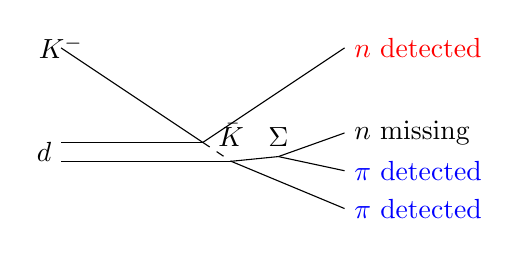
\begin{tikzpicture}[scale=1.2]
    \draw (-1.5,    1) node {$K^-$}--(0,    0);
    \draw (-1.5,    0)--(0,    0);
    \draw (-1.5, -0.2)--(0.3, -0.2);
    \node (d) at (-1.5, -0.1) [left] {$d$};

    \draw (0, 0) -- (0.3, -0.2) [dashed];
    \node (barK) at (0.3, -0.15) [above] {$\bar{K}$};

    \draw ( 1.5,  1.0) node [right] {\textcolor{red}{$n$ detected}}      -- (0,    0);
    
    \draw ( 1.5,  -0.7) node [right] {\textcolor{blue}{$\pi$ detected}} -- (0.3, -0.2);
    
    \draw ( 0.8,  -0.15) node [above] {$\Sigma$}    -- (0.3, -0.2);
    \draw ( 0.8,  -0.15) -- (1.5, 0.1) node [right] {$n$ missing};
    \draw ( 0.8,  -0.15) -- (1.5, -0.3) node [right] {\textcolor{blue}{$\pi$ detected}};    
  \end{tikzpicture}\\
  (a)
  
  \begin{tabular}{cc}
    \begin{minipage}{0.5\hsize}
      \centering
      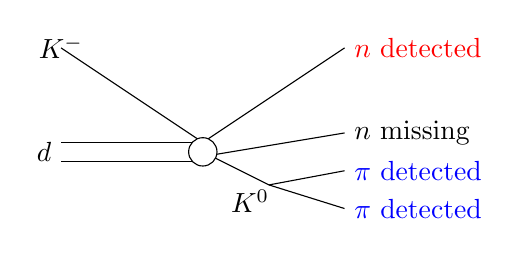
\begin{tikzpicture}[scale=1.2]
        \draw (-1.5,    1) node {$K^-$}--(0,    0);
        \draw (-1.5,    0)--(0,    0);
        \draw (-1.5, -0.2)--(0, -0.2);
        \node (d) at (-1.5, -0.1) [left] {$d$};
        
        \draw ( 1.5,  1.0) node [right] {\textcolor{red}{$n$ detected}}      -- (0,    0);

        
        \node (K0) at (0.5, -0.4) [below] {$K^0$};
        \draw (0, -0.1) -- (0.7, -0.45);
        
        \draw ( 0.0,  -0.15) -- (1.5, 0.1) node [right] {$n$ missing};
        \draw ( 0.7,  -0.45) -- (1.5, -0.3) node [right] {\textcolor{blue}{$\pi$ detected}};
        \draw (1.5,  -0.7) node [right] {\textcolor{blue}{$\pi$ detected}} -- (0.7, -0.45);
        
        \filldraw [fill=white] (0, -0.1) circle [radius=0.15];
      \end{tikzpicture}\\
      (b)
    \end{minipage}
    \begin{minipage}{0.5\hsize}
      \centering
      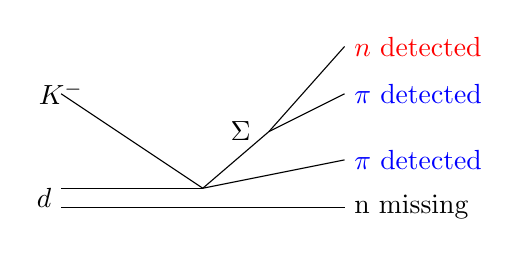
\begin{tikzpicture}[scale=1.2]
        \draw (-1.5,    1) node {$K^-$}--(0,    0);
        \draw (-1.5,    0)--(0,    0);
        \draw (-1.5, -0.2)--(0.3, -0.2);
        \node (d) at (-1.5, -0.1) [left] {$d$};

        \draw ( 1.5,  -0.2) node [right] {n missing} -- (0.3, -0.2);
        \draw ( 1.5,  0.3) node [right] {\textcolor{blue}{$\pi$ detected}}      -- (0,    0);

        \node (barK) at (0.4, 0.4) [above] {$\Sigma$};
        \draw ( 0.7,  0.6) -- (0.0, 0.0);
                
        \draw ( 0.7,  0.6) -- (1.5, 1.5) node [right] {\textcolor{red}{$n$ detected}};
        \draw ( 0.7,  0.6) -- (1.5, 1.0) node [right] {\textcolor{blue}{$\pi$ detected}};    
      \end{tikzpicture}\\
      (c)
    \end{minipage}
  \end{tabular}
  \label{fig:kd_npipin_type}
\end{figure}


The $K^- n \rightarrow n \pi^+ \pi^- n$ final state is identified from the event in which the forward neutron is detected,
as described in Section.\ref{sec:???}.
This final state can be considered to include the three reactions represented in Figure \ref{fig:kd_npipin_type}.
The first is the signal reaction in this analysis where $\bar{K}$ is recoiled backward to $\pi \Sigma$
as shown in Figure.\ref{fig:kd_npipin_type}-(a),
the second is the recoil of $K^0$ decaying directly to $\pi^+ \pi^-$ as shown in Figure \ref{fig:kd_npipin_type}-(b),
and the third is the forward production of $\Sigma$ ($\Sigma_{forward}$) as shown in Figure \ref{fig:kd_npipin_type}-(c),
where forward means that the $n$ decaying from $\Sigma$ are detected by the NC.
Reactions (b) and (c) can be identified by reconstructing $K^0$ and $\Sigma^{\pm}$
from the invariant masses of $\pi^+$ and $\pi^-$ and forward neutrons and $\pi^{\pm}$, respectively,
as shown in Figure.\ref{fig:npipin_IM_fitGauss}.
The invariant mass distributions of $\pi^+ \pi^-$, $n \pi^-$ and $n \pi^+$ are represented in the right, center and left figures respectively.
For the identification of $K^0$ and $\Sigma^{\pm}_{forward}$,
fitting with third-order polynomial function and Gaussian function is used to identify $K^0$ and $\Sigma^{\pm}_{forward}$
in the 3$\sigma$ region of the Gaussian function, which is indicated by the red hatched area.

\begin{figure}[htbp]
  \begin{tabular}{ccc}
    \begin{minipage}{0.33\hsize}
      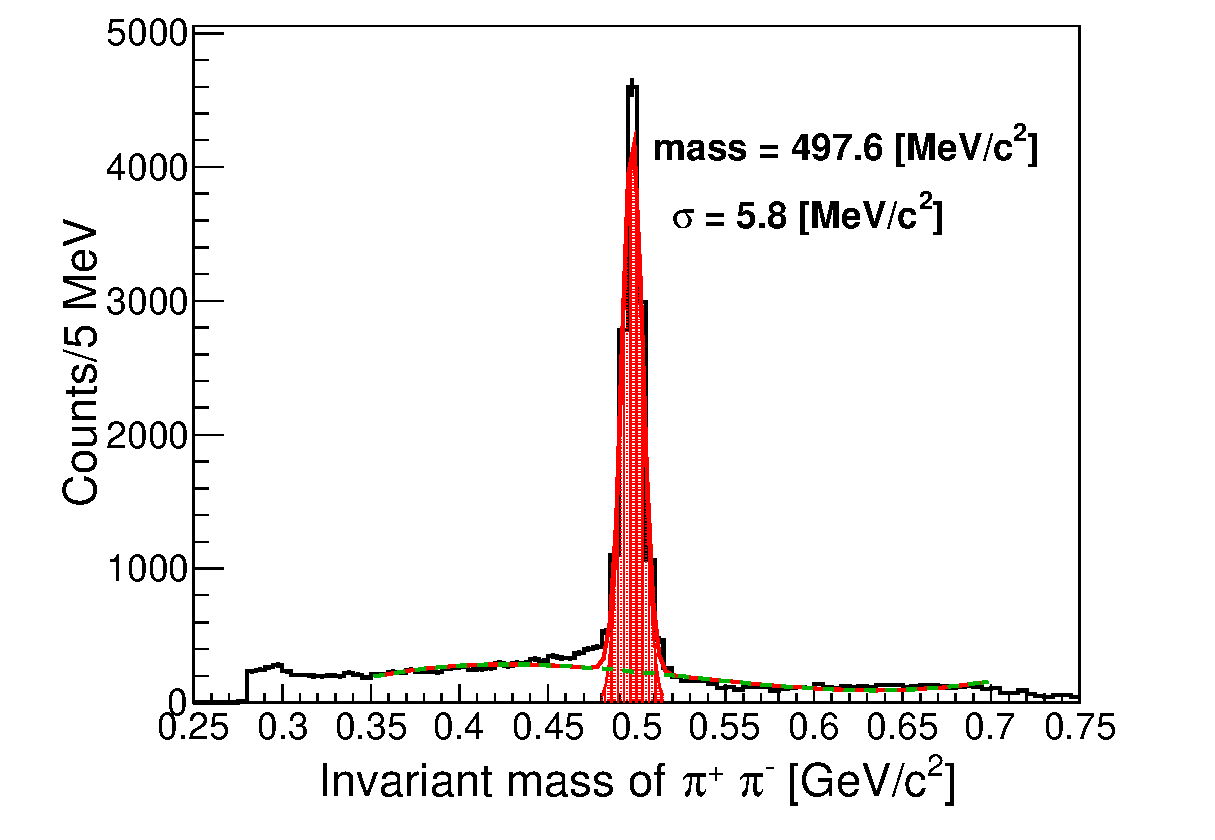
\includegraphics[width=4.5cm]{../pic/Run78/KN_ana_NC170_3sigma/IM_pipi_fitGauss.eps}
    \end{minipage}

    \begin{minipage}{0.33\hsize}
      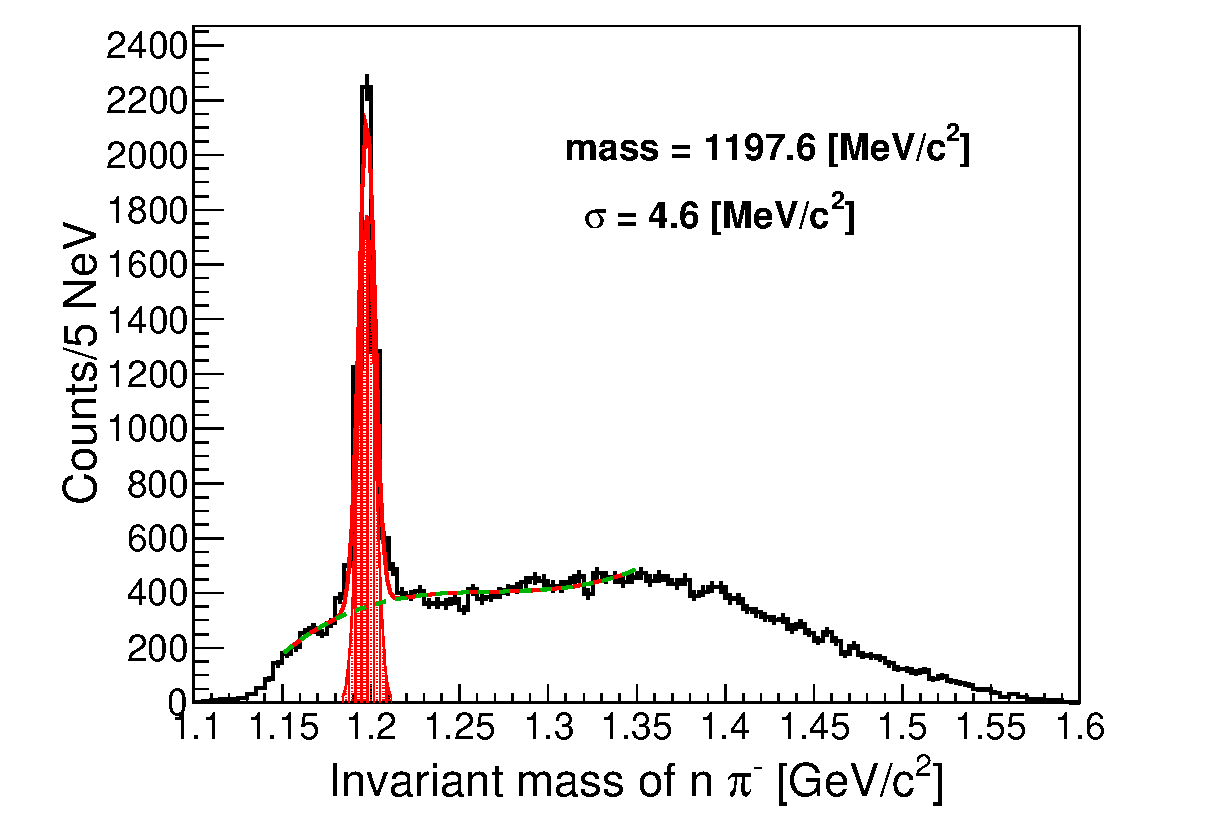
\includegraphics[width=4.5cm]{../pic/Run78/KN_ana_NC170_3sigma/IM_npim_fitGauss.eps}
    \end{minipage}

    \begin{minipage}{0.33\hsize}
      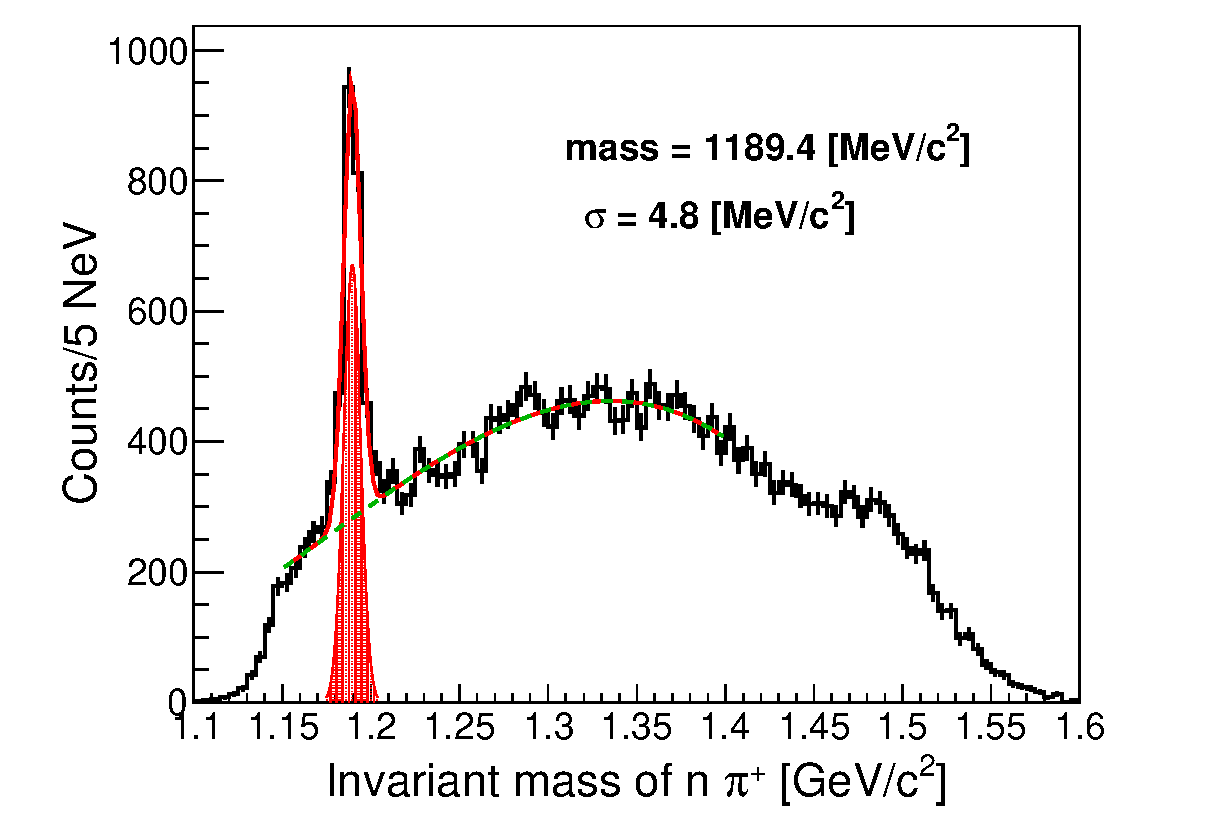
\includegraphics[width=4.5cm]{../pic/Run78/KN_ana_NC170_3sigma/IM_npip_fitGauss.eps}
    \end{minipage}
  \end{tabular}
  \caption{
    These figures show the invariant mass distributions of $\pi^+ \pi^-$,
    $n \pi^-$ and $n \pi^+$ in the $K d \rightarrow n \pi^+ \pi^- n$ event sample from left to right.
    The Gaussian functions and the selection regions for $K^0$ and $\Sigma^{\pm}_{forward}$ are indicated by red hatched area.
    The background third-order polynomial functions are shown as the green dashed lines.
  }
  \label{fig:npipin_IM_fitGauss}
\end{figure}


Rejecting these two reactions leaves a signal reaction in which $\pi \Sigma$ is scattered backward.
This reaction has $\pi^- \Sigma^+$ and $\pi^+ \Sigma^-$ modes, and they must be separated.
The branching ratio of these modes depends on the mass of $\pi \Sigma$, and this separation is performed for each bin of $d(K^-, n)$ missing mass.

\begin{frame}{$d(K^-, n)"nK0"$}
  \begin{figure}
    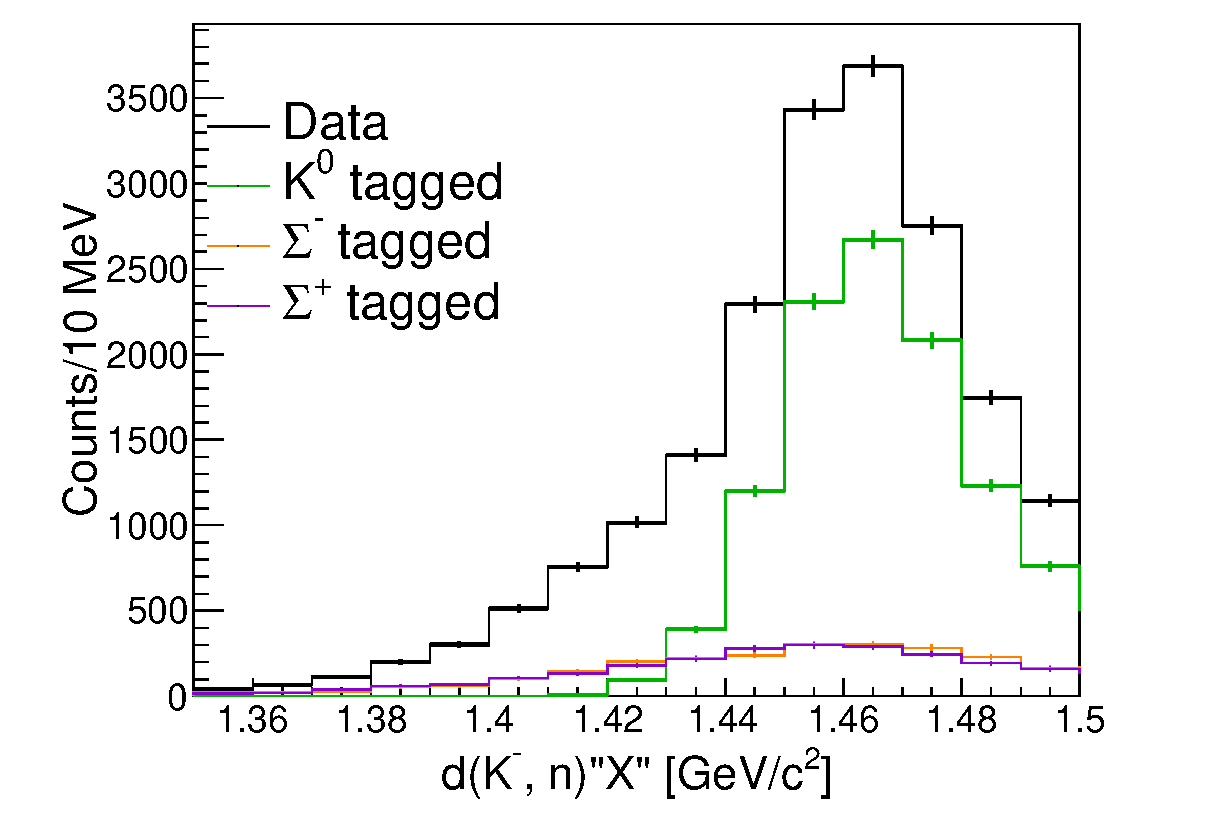
\includegraphics[width=8cm]{../pic/Run78/KN_ana_NC170_2sigma/KN_MM_all.eps}
  \end{figure}
\end{frame}


Figure \ref{fig:KN_MM_npipin} shows the $d(K^-, n)$ missing masses in which the $K^- d \rightarrow n \pi^+ \pi^- n$ final state has been identified.
On the left, all events, those identifying $K^0$, those identifying $\Sigma^+_{forward}$, and those identifying $\Sigma^-_{forward}$
are indicated by black, green, red, and blue lines, respectively.
The right figure shows the signal spectrum, subtracting the events identified as $K^0$ or $\Sigma^{\pm}_{forward}$ from all events.

To separate these events,
we generated template events using a Geant4 Monte Carlo simulation and decomposed the reactions by fitting their spectra with templates.
This decomposition was applied not only to the signal but also to the background reactions.
The procedures used in this decomposition are described in detail in Section \ref{sec:template_fitting}
The estimation of the detector resolution used in this simulation is described in detail in Appendix \ref{chapter:detector_resolution}.


\subsection{Template fitting} \label{sec:template_fitting}
\newcommand{\IMfitChiSquare}{1077.4}
\newcommand{\IMfitNDF}{352}
\newcommand{\IMfitChiNDF}{3.06}

\newcommand{\KzeroFitChi}{275.2}
\newcommand{\KzeroFitNDF}{43}
\newcommand{\KzeroFitChiNDF}{6.40}

\newcommand{\KzeroOneStepRatio}{80.9 \pm 1.3\%}
\newcommand{\KzeroTwoStepRatio}{11.5 \pm 1.0\%}
\newcommand{\KzeroLsRatio}{7.7 \pm 0.6\%}


% \section{Template fitting of $K^- d \rightarrow n \pi^+ \pi^- n$ events} \label{sec:tempFit}
% \subsection{Backward $\pi^{\mp}\Sigma^{\pm}$ event selection} \label{sec:backward_piSigma}
\begin{figure}
  \centering
  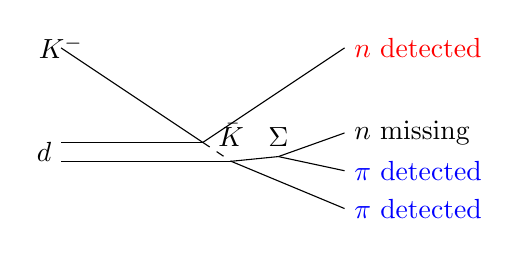
\begin{tikzpicture}[scale=1.2]
    \draw (-1.5,    1) node {$K^-$}--(0,    0);
    \draw (-1.5,    0)--(0,    0);
    \draw (-1.5, -0.2)--(0.3, -0.2);
    \node (d) at (-1.5, -0.1) [left] {$d$};

    \draw (0, 0) -- (0.3, -0.2) [dashed];
    \node (barK) at (0.3, -0.15) [above] {$\bar{K}$};

    \draw ( 1.5,  1.0) node [right] {\textcolor{red}{$n$ detected}}      -- (0,    0);
    
    \draw ( 1.5,  -0.7) node [right] {\textcolor{blue}{$\pi$ detected}} -- (0.3, -0.2);
    
    \draw ( 0.8,  -0.15) node [above] {$\Sigma$}    -- (0.3, -0.2);
    \draw ( 0.8,  -0.15) -- (1.5, 0.1) node [right] {$n$ missing};
    \draw ( 0.8,  -0.15) -- (1.5, -0.3) node [right] {\textcolor{blue}{$\pi$ detected}};    
  \end{tikzpicture}\\
  (a)
  
  \begin{tabular}{cc}
    \begin{minipage}{0.5\hsize}
      \centering
      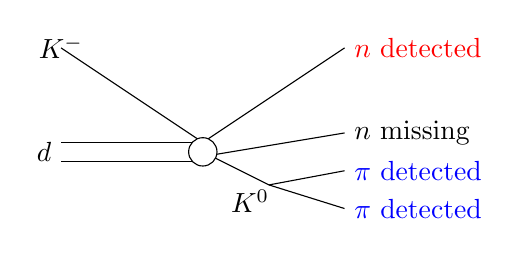
\begin{tikzpicture}[scale=1.2]
        \draw (-1.5,    1) node {$K^-$}--(0,    0);
        \draw (-1.5,    0)--(0,    0);
        \draw (-1.5, -0.2)--(0, -0.2);
        \node (d) at (-1.5, -0.1) [left] {$d$};
        
        \draw ( 1.5,  1.0) node [right] {\textcolor{red}{$n$ detected}}      -- (0,    0);

        
        \node (K0) at (0.5, -0.4) [below] {$K^0$};
        \draw (0, -0.1) -- (0.7, -0.45);
        
        \draw ( 0.0,  -0.15) -- (1.5, 0.1) node [right] {$n$ missing};
        \draw ( 0.7,  -0.45) -- (1.5, -0.3) node [right] {\textcolor{blue}{$\pi$ detected}};
        \draw (1.5,  -0.7) node [right] {\textcolor{blue}{$\pi$ detected}} -- (0.7, -0.45);
        
        \filldraw [fill=white] (0, -0.1) circle [radius=0.15];
      \end{tikzpicture}\\
      (b)
    \end{minipage}
    \begin{minipage}{0.5\hsize}
      \centering
      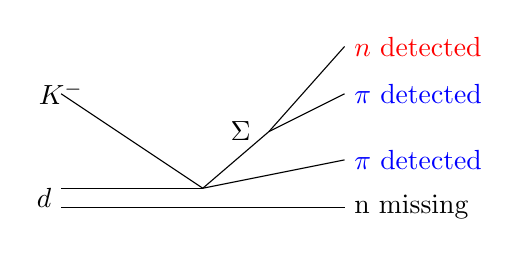
\begin{tikzpicture}[scale=1.2]
        \draw (-1.5,    1) node {$K^-$}--(0,    0);
        \draw (-1.5,    0)--(0,    0);
        \draw (-1.5, -0.2)--(0.3, -0.2);
        \node (d) at (-1.5, -0.1) [left] {$d$};

        \draw ( 1.5,  -0.2) node [right] {n missing} -- (0.3, -0.2);
        \draw ( 1.5,  0.3) node [right] {\textcolor{blue}{$\pi$ detected}}      -- (0,    0);

        \node (barK) at (0.4, 0.4) [above] {$\Sigma$};
        \draw ( 0.7,  0.6) -- (0.0, 0.0);
                
        \draw ( 0.7,  0.6) -- (1.5, 1.5) node [right] {\textcolor{red}{$n$ detected}};
        \draw ( 0.7,  0.6) -- (1.5, 1.0) node [right] {\textcolor{blue}{$\pi$ detected}};    
      \end{tikzpicture}\\
      (c)
    \end{minipage}
  \end{tabular}
  \label{fig:kd_npipin_type}
\end{figure}


The $K^- n \rightarrow n \pi^+ \pi^- n$ final state is identified from the event in which the forward neutron is detected,
as described in Section.\ref{sec:???}.
This final state can be considered to include the three reactions represented in Figure \ref{fig:kd_npipin_type}.
The first is the signal reaction in this analysis where $\bar{K}$ is recoiled backward to $\pi \Sigma$
as shown in Figure.\ref{fig:kd_npipin_type}-(a),
the second is the recoil of $K^0$ decaying directly to $\pi^+ \pi^-$ as shown in Figure \ref{fig:kd_npipin_type}-(b),
and the third is the forward production of $\Sigma$ ($\Sigma_{forward}$) as shown in Figure \ref{fig:kd_npipin_type}-(c),
where forward means that the $n$ decaying from $\Sigma$ are detected by the NC.
Reactions (b) and (c) can be identified by reconstructing $K^0$ and $\Sigma^{\pm}$
from the invariant masses of $\pi^+$ and $\pi^-$ and forward neutrons and $\pi^{\pm}$, respectively,
as shown in Figure.\ref{fig:npipin_IM_fitGauss}.
The invariant mass distributions of $\pi^+ \pi^-$, $n \pi^-$ and $n \pi^+$ are represented in the right, center and left figures respectively.
For the identification of $K^0$ and $\Sigma^{\pm}_{forward}$,
fitting with third-order polynomial function and Gaussian function is used to identify $K^0$ and $\Sigma^{\pm}_{forward}$
in the 3$\sigma$ region of the Gaussian function, which is indicated by the red hatched area.

\begin{figure}[htbp]
  \begin{tabular}{ccc}
    \begin{minipage}{0.33\hsize}
      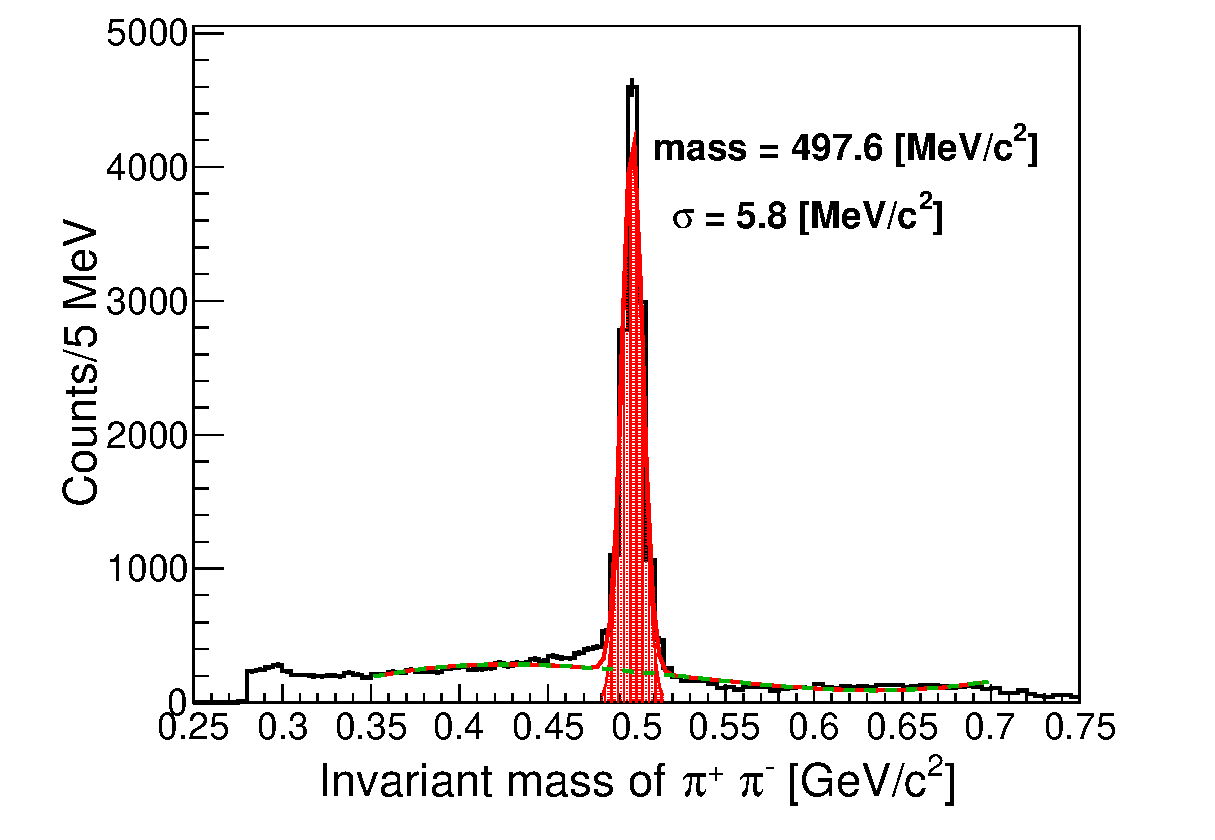
\includegraphics[width=4.5cm]{../pic/Run78/KN_ana_NC170_3sigma/IM_pipi_fitGauss.eps}
    \end{minipage}

    \begin{minipage}{0.33\hsize}
      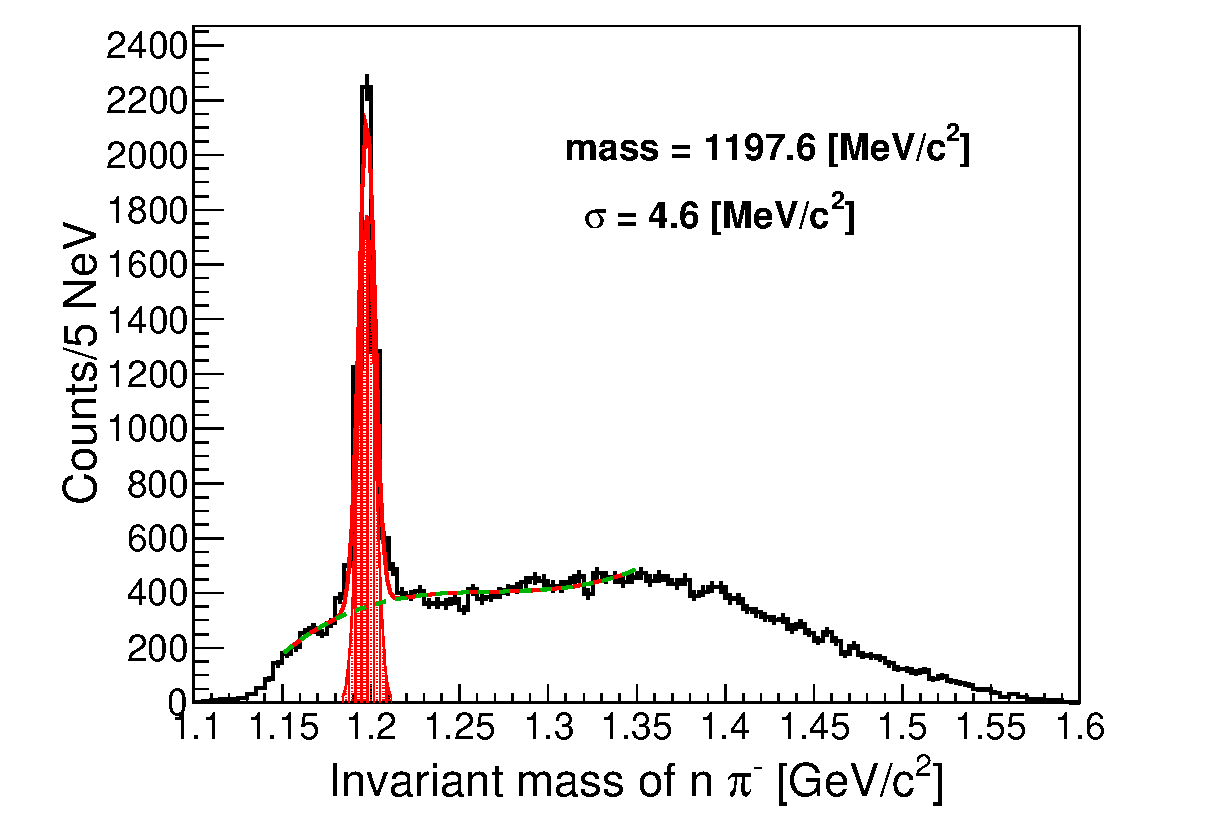
\includegraphics[width=4.5cm]{../pic/Run78/KN_ana_NC170_3sigma/IM_npim_fitGauss.eps}
    \end{minipage}

    \begin{minipage}{0.33\hsize}
      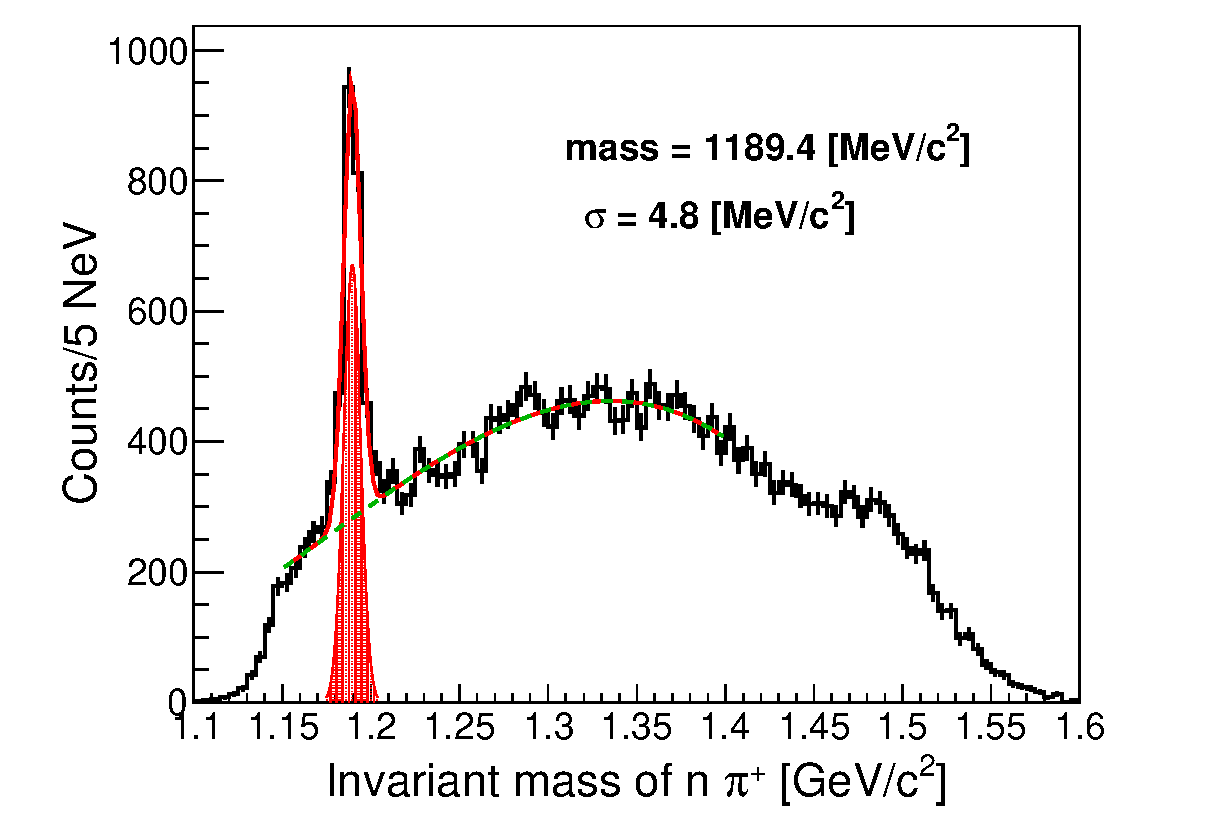
\includegraphics[width=4.5cm]{../pic/Run78/KN_ana_NC170_3sigma/IM_npip_fitGauss.eps}
    \end{minipage}
  \end{tabular}
  \caption{
    These figures show the invariant mass distributions of $\pi^+ \pi^-$,
    $n \pi^-$ and $n \pi^+$ in the $K d \rightarrow n \pi^+ \pi^- n$ event sample from left to right.
    The Gaussian functions and the selection regions for $K^0$ and $\Sigma^{\pm}_{forward}$ are indicated by red hatched area.
    The background third-order polynomial functions are shown as the green dashed lines.
  }
  \label{fig:npipin_IM_fitGauss}
\end{figure}


Rejecting these two reactions leaves a signal reaction in which $\pi \Sigma$ is scattered backward.
This reaction has $\pi^- \Sigma^+$ and $\pi^+ \Sigma^-$ modes, and they must be separated.
The branching ratio of these modes depends on the mass of $\pi \Sigma$, and this separation is performed for each bin of $d(K^-, n)$ missing mass.

\begin{frame}{$d(K^-, n)"nK0"$}
  \begin{figure}
    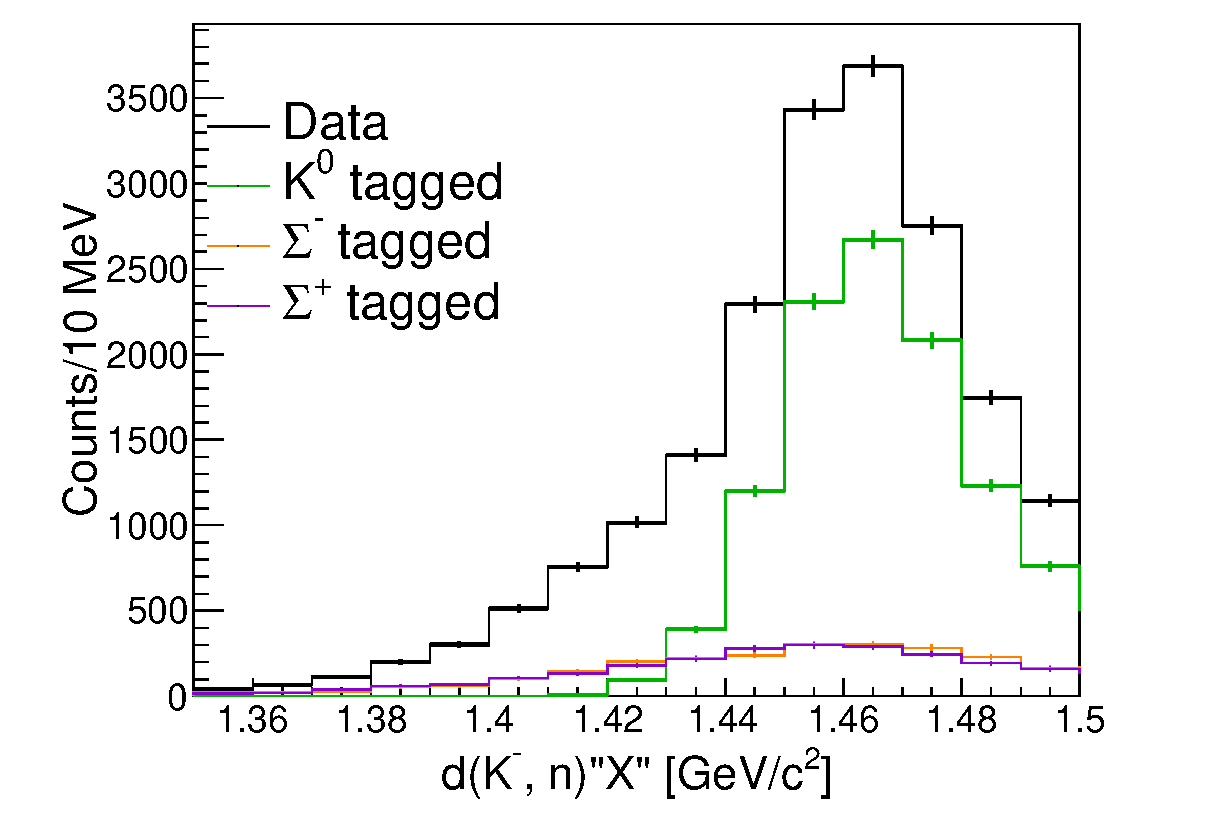
\includegraphics[width=8cm]{../pic/Run78/KN_ana_NC170_2sigma/KN_MM_all.eps}
  \end{figure}
\end{frame}


Figure \ref{fig:KN_MM_npipin} shows the $d(K^-, n)$ missing masses in which the $K^- d \rightarrow n \pi^+ \pi^- n$ final state has been identified.
On the left, all events, those identifying $K^0$, those identifying $\Sigma^+_{forward}$, and those identifying $\Sigma^-_{forward}$
are indicated by black, green, red, and blue lines, respectively.
The right figure shows the signal spectrum, subtracting the events identified as $K^0$ or $\Sigma^{\pm}_{forward}$ from all events.

To separate these events,
we generated template events using a Geant4 Monte Carlo simulation and decomposed the reactions by fitting their spectra with templates.
This decomposition was applied not only to the signal but also to the background reactions.
The procedures used in this decomposition are described in detail in Section \ref{sec:template_fitting}
The estimation of the detector resolution used in this simulation is described in detail in Appendix \ref{chapter:detector_resolution}.



\subsection{Template fitting} \label{sec:template_fitting}
\newcommand{\IMfitChiSquare}{1077.4}
\newcommand{\IMfitNDF}{352}
\newcommand{\IMfitChiNDF}{3.06}

\newcommand{\KzeroFitChi}{275.2}
\newcommand{\KzeroFitNDF}{43}
\newcommand{\KzeroFitChiNDF}{6.40}

\newcommand{\KzeroOneStepRatio}{80.9 \pm 1.3\%}
\newcommand{\KzeroTwoStepRatio}{11.5 \pm 1.0\%}
\newcommand{\KzeroLsRatio}{7.7 \pm 0.6\%}


% \section{Template fitting of $K^- d \rightarrow n \pi^+ \pi^- n$ events} \label{sec:tempFit}
% \subsection{Backward $\pi^{\mp}\Sigma^{\pm}$ event selection} \label{sec:backward_piSigma}
\input{analysis/template_fitting/figs/kd_npipin_type}

The $K^- n \rightarrow n \pi^+ \pi^- n$ final state is identified from the event in which the forward neutron is detected,
as described in Section.\ref{sec:???}.
This final state can be considered to include the three reactions represented in Figure \ref{fig:kd_npipin_type}.
The first is the signal reaction in this analysis where $\bar{K}$ is recoiled backward to $\pi \Sigma$
as shown in Figure.\ref{fig:kd_npipin_type}-(a),
the second is the recoil of $K^0$ decaying directly to $\pi^+ \pi^-$ as shown in Figure \ref{fig:kd_npipin_type}-(b),
and the third is the forward production of $\Sigma$ ($\Sigma_{forward}$) as shown in Figure \ref{fig:kd_npipin_type}-(c),
where forward means that the $n$ decaying from $\Sigma$ are detected by the NC.
Reactions (b) and (c) can be identified by reconstructing $K^0$ and $\Sigma^{\pm}$
from the invariant masses of $\pi^+$ and $\pi^-$ and forward neutrons and $\pi^{\pm}$, respectively,
as shown in Figure.\ref{fig:npipin_IM_fitGauss}.
The invariant mass distributions of $\pi^+ \pi^-$, $n \pi^-$ and $n \pi^+$ are represented in the right, center and left figures respectively.
For the identification of $K^0$ and $\Sigma^{\pm}_{forward}$,
fitting with third-order polynomial function and Gaussian function is used to identify $K^0$ and $\Sigma^{\pm}_{forward}$
in the 3$\sigma$ region of the Gaussian function, which is indicated by the red hatched area.

\input{analysis/template_fitting/figs/npipin_IM_fitGauss}

Rejecting these two reactions leaves a signal reaction in which $\pi \Sigma$ is scattered backward.
This reaction has $\pi^- \Sigma^+$ and $\pi^+ \Sigma^-$ modes, and they must be separated.
The branching ratio of these modes depends on the mass of $\pi \Sigma$, and this separation is performed for each bin of $d(K^-, n)$ missing mass.

\input{analysis/template_fitting/figs/KN_MM}

Figure \ref{fig:KN_MM_npipin} shows the $d(K^-, n)$ missing masses in which the $K^- d \rightarrow n \pi^+ \pi^- n$ final state has been identified.
On the left, all events, those identifying $K^0$, those identifying $\Sigma^+_{forward}$, and those identifying $\Sigma^-_{forward}$
are indicated by black, green, red, and blue lines, respectively.
The right figure shows the signal spectrum, subtracting the events identified as $K^0$ or $\Sigma^{\pm}_{forward}$ from all events.

To separate these events,
we generated template events using a Geant4 Monte Carlo simulation and decomposed the reactions by fitting their spectra with templates.
This decomposition was applied not only to the signal but also to the background reactions.
The procedures used in this decomposition are described in detail in Section \ref{sec:template_fitting}
The estimation of the detector resolution used in this simulation is described in detail in Appendix \ref{chapter:detector_resolution}.



\subsection{Template fitting} \label{sec:template_fitting}
\input{discussion/template_fitting/params}

% \section{Template fitting of $K^- d \rightarrow n \pi^+ \pi^- n$ events} \label{sec:tempFit}
% \subsection{Backward $\pi^{\mp}\Sigma^{\pm}$ event selection} \label{sec:backward_piSigma}
\input{discussion/template_fitting/backward_piSigma_selection}

\subsection{Template fitting} \label{sec:template_fitting}
\input{discussion/template_fitting/template_fitting}

%% \input{discussion/template_fitting/MC_data}
%% \input{discussion/template_fitting/procedure}
%% \input{discussion/template_fitting/fit_K0}



%% \subsection{Generated data by Monte Calro simulation} \label{subsec:tempFit_MCdata}
\input{discussion/template_fitting/reactions}
Since the $K^- d\rightarrow n \pi^+ \pi^- n$ event is expected to contain 3 type reactions, (\ref{reaction:prodK0})-(\ref{2step:piS}),
we obtain the $d(K^-, n)"\pi^{\mp}\Sigma^{\pm}"$ event rejecting $K^0$ and $\Sigma^{\pm}_{forward}$ in $K^- d \rightarrow n \pi^+ \pi^- n$ event.

We perform template fitting using data reproduced using Monte Carlo simulation (geant4) to decompose into $\pi^-\Sigma^+$ and $\pi^+\Sigma^-$ modes.
In this subsection, we explain how we reproduce the data using geant4 simulation.

The $K^0$ production in (\ref{reaction:prodK0}) is simply the so-called quasi-elastic scattering,
in which an initial $K^-$ reacts with a proton and is converted into $K^0$ and a neutron, where the residual neutron is a spectator and its momentum is the Fermi momentum.
This reaction causes the scattering angles of the reacting protons and $K^-$ to be distributed in a way that reproduces the past experiment of one nucleon scattering \cite{KP_K0n},
and the momentum of the spectator is also distributed in a way that reproduces the past experiment \cite{d_fermi_ex}.
In the case of $\Sigma^{\pm}_{forward}$ production in (\ref{reaction:prodSigma}), the angular distribution of the past experiment\cite{KP_CEX_1GeV} is simulated in the same way.

In the $K^0$ produced event (\ref{reaction:prodK0}), in addition to 1-step reaction described above, events such as a 2-step and direct $\Lambda(1520)$ production are observed.
So, we generate data of these reaction.
In the case of 2-step reaction, the momentum of recoiled $\bar{K}$ is small and the scattering data of such $\bar{K}$ and nucleon are a few,
so the angular distribution and other details are not known.
Therefore, the MC data is generated assuming that the scattering of recoiled $\bar{K}$ and nucleons is isotropic. 
In the case of direct $\Lambda(1520)$ production also no data.
Therefore, this data was isotropically scattered $K^-d \rightarrow n \Lambda(1520)$ and $\Lambda(1520)$ decayed to $n$ and $K^0$.

Next, we explain the main signal (\ref{2step:piS}), which is the backward $\pi\Sigma$ generation.
Since there is no data on the invariant mass of $\pi\Sigma$, it is generated as a uniform distribution from the $\bar{K}N$ threshold, whose lineshape is determined by template fitting.
There is also no data on the scattering angle of $\pi\Sigma$,
but since the $\bar{K}N\rightarrow \pi\Sigma$ scattering is expected to be $S$-wave in this reaction,
we assume that it is isotropic and generate MC data.

In summary, the following seven MC data are used for template fitting.
\input{discussion/template_fitting/MC_data_list}

%% \subsection{Procedure of template fitting}
\input{discussion/template_fitting/figs/fit_IM}
\input{discussion/template_fitting/figs/fit_KNpi_MM_all}

In this subsection, we explain procedure of template fitting, whose main purpose is decomposition of $\pi^- \Sigma^+$ and $\pi^+ \Sigma^-$ modes.
Template fitting is divided into two stages, one fitting to estimate the amount of background for $K^0$ and $\Sigma_{forward}$ production,
the other to separate $\pi^-\Sigma^+$ and $\pi^+\Sigma^-$ modes.
These fittings are performed using fitting with the likelihood method on a finite sample generated by Monte Carlo method\cite{temp_fit}.
There is no $\chi^2$ in this fitting,
but there is a value of $-2\log\Lambda$ that asymptotically approaches the $\chi^2$ when the number of samples become infinite, and the fitting is evaluated with this value.
Here, $\Lambda$ is the likelihood.

The first fitting is performed using the invariant mass distributions of $\pi^+ \pi^-$, $n \pi^+$ and $n \pi^-$ in the event that $K^-d \rightarrow n \pi^+ \pi^- n$ final state.
The $K^0$, $\Sigma^+$ and $\Sigma^-$ productions create peaks in the respective invariant mass distributions as shown in Fig.\ref{fig:fit_IM}.
The distributions reconstructed by fitting are also plotted in the same figure.
The bold line represents the case of backward $\pi \Sigma$ production of signal, with red and blue representing the $\pi^- \Sigma^+$ and $\pi^-\Sigma^+$ modes, respectively.
The other green, purple and orange lines represent the background for $K^0$, $\Sigma^-_{forward}$ and $\Sigma^+_{forward}$ production, respectively.
This fitting of $-2\log\Lambda$ is \IMfitChiSquare.
Degrees freedom is the number of bin with data, and $-2\log\Lambda/NDF \sim $\IMfitChiNDF. 
% For this purpose, the distribution is fitted with a Gaussian and a 5-th polynomial function, and the rejection region is defined by the 3$\sigma$ of the Gaussian.

\input{discussion/template_fitting/figs/fit_KNpi_MM}
\input{discussion/template_fitting/figs/tempFit_KNpi_Chi2}

The fitting to separate the $\pi^-\Sigma^+$ and $\pi^+\Sigma^-$ modes is performed for events from $K^-- d \rightarrow n \pi^+ \pi- n$, excluding $K^0 $and $\Sigma^{\pm}_{forward}$ production.
However, the background leakage is estimated by scaling the distribution reconstructed in the MC simulation by the intensity estimated by the invariant mass fitting.
This fitting is performed each bin of the missing mass of $d(K^-, n)$, since the scattering amplitude of $\bar{K}N \rightarrow \pi \Sigma$ depends on the $\pi \Sigma$ invariant mass.
For this fitting we use the $d(K^-, n \pi^-)$ and $d(K^-, n \pi^+)$ missing masses as shown in Fig.\ref{fig:fit_KNpi_MM_all}.
This figure shows the sum of the $d(K^- , n)$ bins.
The bottom left figure shows a two-dimensional figure of the $d(K^-, n \pi^-)$ and $d(K^-, n \pi^+)$ missing masses on the horizontal and vertical axes, respectively.
The top and right figures show the projections of the respective axes.
The missing mass of $d(K^-, n \pi)$ makes a peak at $\Sigma$ for the correct combination for the missing $\Sigma$, but is widely distributed in the kinematic region for the opposite charge.
For example, for $d(K^-, n \pi^-)$, the $\pi^- \Sigma^+$ mode has a peak structure as shown by the red line,
whereas the $\pi^+ \Sigma^-$ mode has a widely distributed structure as shown by the blue line.

Fig.\ref{fig:fit_KNpi_MM} shows the results for the fitting of each bin of $d(K^-, n)$ separately.
Fig.\ref{fig:tempFit_KNpi_Chi2} shows the $-2\log\Lambda$ and $-2\log\Lambda/NDF$ of this fitting in each $d(K^-, n)$ bin in black and red, respectively.

Fitting to estimate background and to separate $\pi^- \Sigma^+$ and $\pi^+ \Sigma^-$ modes cannot be performed simultaneously as they use different event samples.
They are therefore repeated in the following steps.

First, the separation of $\pi^- \Sigma^+$ and $\pi^+ \Sigma^-$ modes is performed without considering the background.
The obtained distribution of backward $\pi^{\mp} \Sigma^{\pm}$ modes is used for fitting to estimate the background,
which is then fed back into the fitting of the separation of $\pi^- \Sigma^+$ and $\pi^+ \Sigma^-$ modes.
After five iterations of this procedure, fitting is performed considering 2-step and direct $\Lambda(1520)$ generation for $K^0$ generation, which is described in the Appendix.\ref{apendix:K0_event}.
Finally, fitting of the separation of the $\pi^- \Sigma^+$ and $\pi^+ \Sigma^-$ modes is performed to obtain the final $\pi \Sigma$ spectrum as shown in Fig.\ref{fig:piS_num}..

\input{discussion/template_fitting/figs/piS_num}


%% \begin{frame}{Template fitting to decompose $K^0$ production}
  \begin{figure}
    \centering
    Invariant mass of $n K^0$\\
    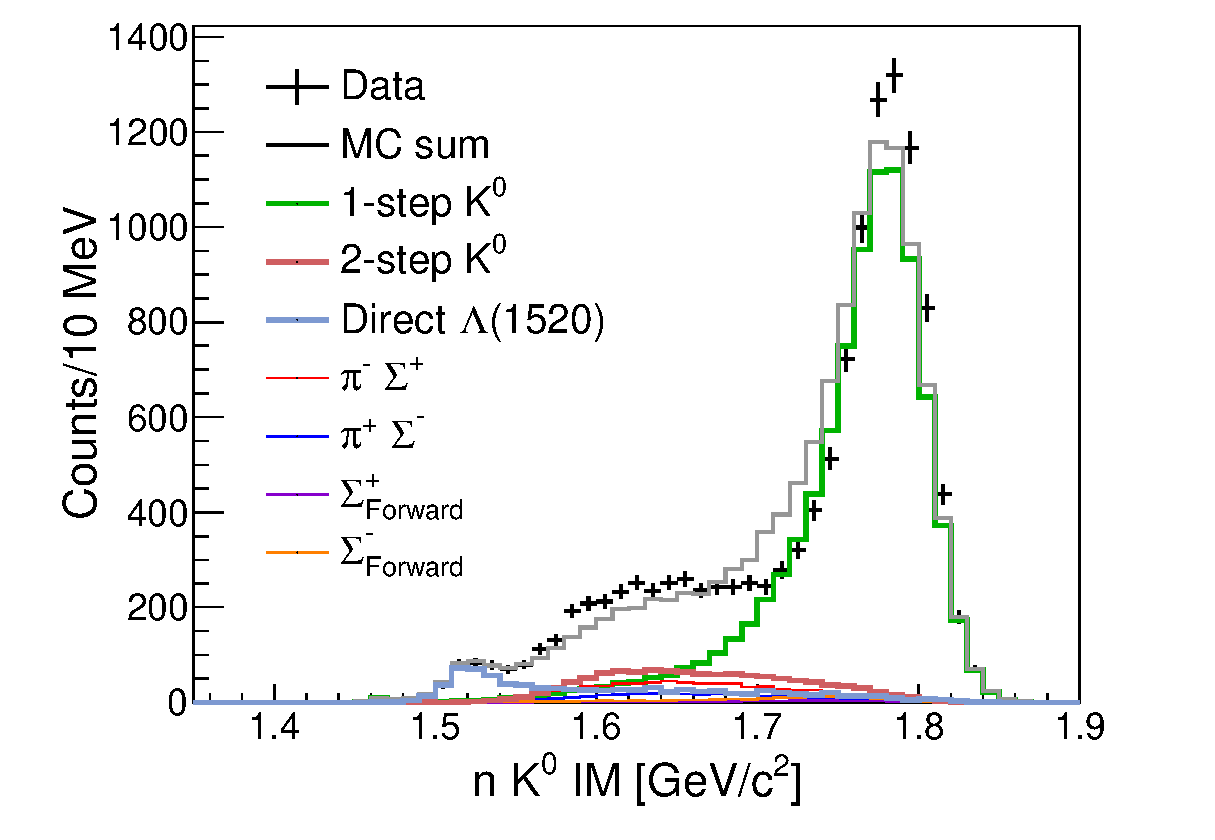
\includegraphics[width=7.5cm]{../pic/Dron/K0_ana/npipi_IM_K0.eps}
  \end{figure}
  \centering
  2-step like component is seen about 11.5\%.\\
  Direct-$\Lambda(1520)$ prod. is seen about 7.7\%.\\
\end{frame}




%% \subsection{Generated data by Monte Calro simulation} \label{subsec:tempFit_MCdata}
\begin{eqnarray}
  & &  K^- d \rightarrow n K^0 n \label{reaction:prodK0} \\
  & &  K^- d \rightarrow \pi^\mp \Sigma^\pm n_{forward} \label{2step:piS}\\
  & &  K^- d \rightarrow \pi^\mp \Sigma^\pm n_{missing} \label{reaction:prodSigma}
\end{eqnarray}

Since the $K^- d\rightarrow n \pi^+ \pi^- n$ event is expected to contain 3 type reactions, (\ref{reaction:prodK0})-(\ref{2step:piS}),
we obtain the $d(K^-, n)"\pi^{\mp}\Sigma^{\pm}"$ event rejecting $K^0$ and $\Sigma^{\pm}_{forward}$ in $K^- d \rightarrow n \pi^+ \pi^- n$ event.

We perform template fitting using data reproduced using Monte Carlo simulation (geant4) to decompose into $\pi^-\Sigma^+$ and $\pi^+\Sigma^-$ modes.
In this subsection, we explain how we reproduce the data using geant4 simulation.

The $K^0$ production in (\ref{reaction:prodK0}) is simply the so-called quasi-elastic scattering,
in which an initial $K^-$ reacts with a proton and is converted into $K^0$ and a neutron, where the residual neutron is a spectator and its momentum is the Fermi momentum.
This reaction causes the scattering angles of the reacting protons and $K^-$ to be distributed in a way that reproduces the past experiment of one nucleon scattering \cite{KP_K0n},
and the momentum of the spectator is also distributed in a way that reproduces the past experiment \cite{d_fermi_ex}.
In the case of $\Sigma^{\pm}_{forward}$ production in (\ref{reaction:prodSigma}), the angular distribution of the past experiment\cite{KP_CEX_1GeV} is simulated in the same way.

In the $K^0$ produced event (\ref{reaction:prodK0}), in addition to 1-step reaction described above, events such as a 2-step and direct $\Lambda(1520)$ production are observed.
So, we generate data of these reaction.
In the case of 2-step reaction, the momentum of recoiled $\bar{K}$ is small and the scattering data of such $\bar{K}$ and nucleon are a few,
so the angular distribution and other details are not known.
Therefore, the MC data is generated assuming that the scattering of recoiled $\bar{K}$ and nucleons is isotropic. 
In the case of direct $\Lambda(1520)$ production also no data.
Therefore, this data was isotropically scattered $K^-d \rightarrow n \Lambda(1520)$ and $\Lambda(1520)$ decayed to $n$ and $K^0$.

Next, we explain the main signal (\ref{2step:piS}), which is the backward $\pi\Sigma$ generation.
Since there is no data on the invariant mass of $\pi\Sigma$, it is generated as a uniform distribution from the $\bar{K}N$ threshold, whose lineshape is determined by template fitting.
There is also no data on the scattering angle of $\pi\Sigma$,
but since the $\bar{K}N\rightarrow \pi\Sigma$ scattering is expected to be $S$-wave in this reaction,
we assume that it is isotropic and generate MC data.

In summary, the following seven MC data are used for template fitting.
\begin{itemize}
  \item About $K^0$ production reaction
  \begin{itemize}
  \item
    $ K^- d \rightarrow n_{forward} K^0 n_{spectator}$ \hspace{\fill} ($K^0$ 1-step)
  \item
    $K^- d \rightarrow n_{forward} (K^0 n)_{isotropic}$ \hspace{\fill} ($K^0$ 2-step)
  \item
    $K^- d \rightarrow n \Lambda(1520) \rightarrow n K^0 n$ \hspace{\fill} (direct $\Lambda(1520)$)
  \end{itemize}
\item About $\Sigma_{forward}$ production reaction
  \begin{itemize}
  \item
    $K^- d \rightarrow \Sigma^+ \pi^- n_{spectator} \rightarrow n_{forward} \pi^+ \pi^- n_{spectator}$ \hspace{\fill} ($\Sigma^+$ 1-step)
  \item
    $K^- d \rightarrow \Sigma^- \pi^+ n_{spectator} \rightarrow n_{forward} \pi^- \pi^+ n_{spectator}$ \hspace{\fill} ($\Sigma^-$ 1-step)
  \end{itemize}
\item About backward $\pi \Sigma$ production reaction
  \begin{itemize}
  \item
    $K^- d \rightarrow n_{forward} \pi^- \Sigma^+$ \hspace{\fill} (backward $\pi^- \Sigma^+$)
  \item
    $K^- d \rightarrow n_{forward} \pi^+ \Sigma^-$ \hspace{\fill} (backward $\pi^+ \Sigma^-$)
  \end{itemize}
\end{itemize}


%% \subsection{Procedure of template fitting}
\begin{frame}{Template fitting to evaluate background}
  \centering
  $d(K^, n \pi^- \pi^+)"n"$ event.
  \begin{tabular}{ccc}
    \begin{minipage}{0.33\hsize}
      \centering
      $\pi^+ \pi^-$ IM\\
      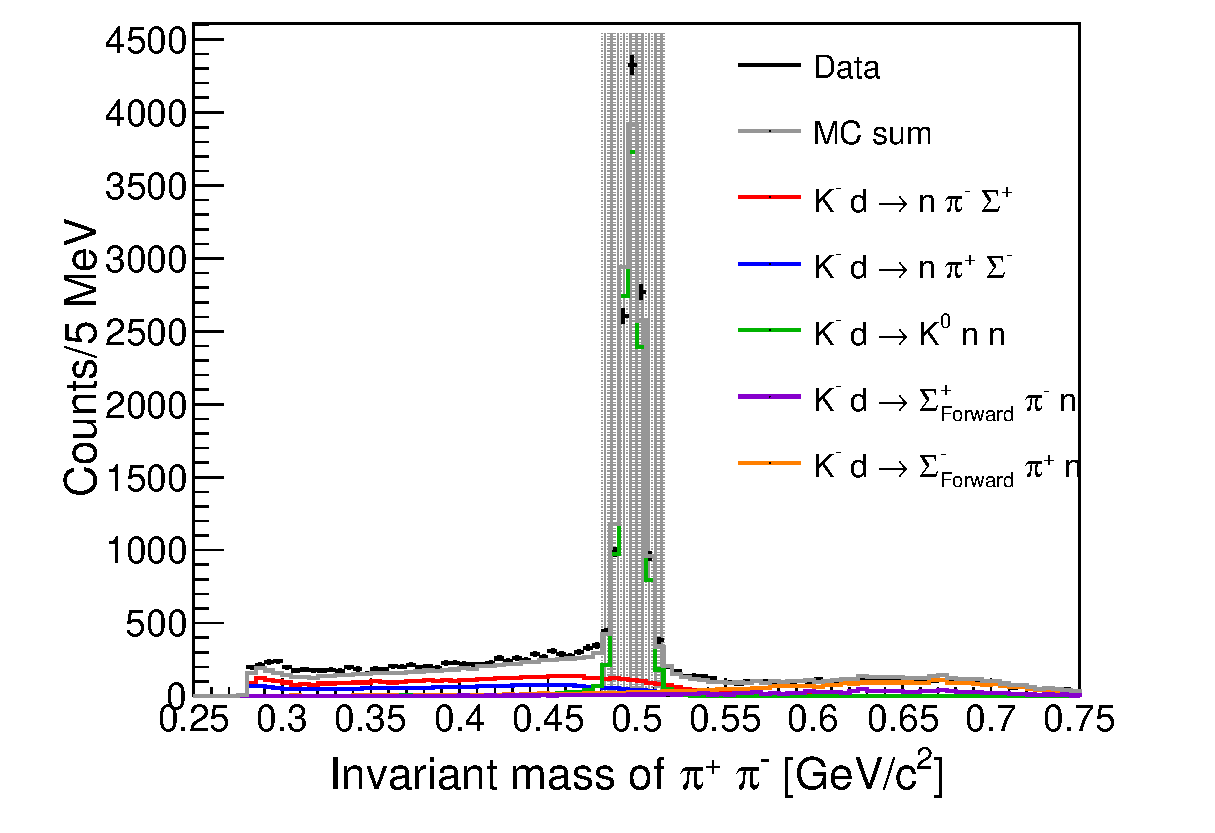
\includegraphics[width=4cm]{../pic/Dron/KN_ana/IM_pipi.eps}
    \end{minipage}
    \begin{minipage}{0.33\hsize}
      \centering
      $n_{forward} \pi^+$ IM\\
      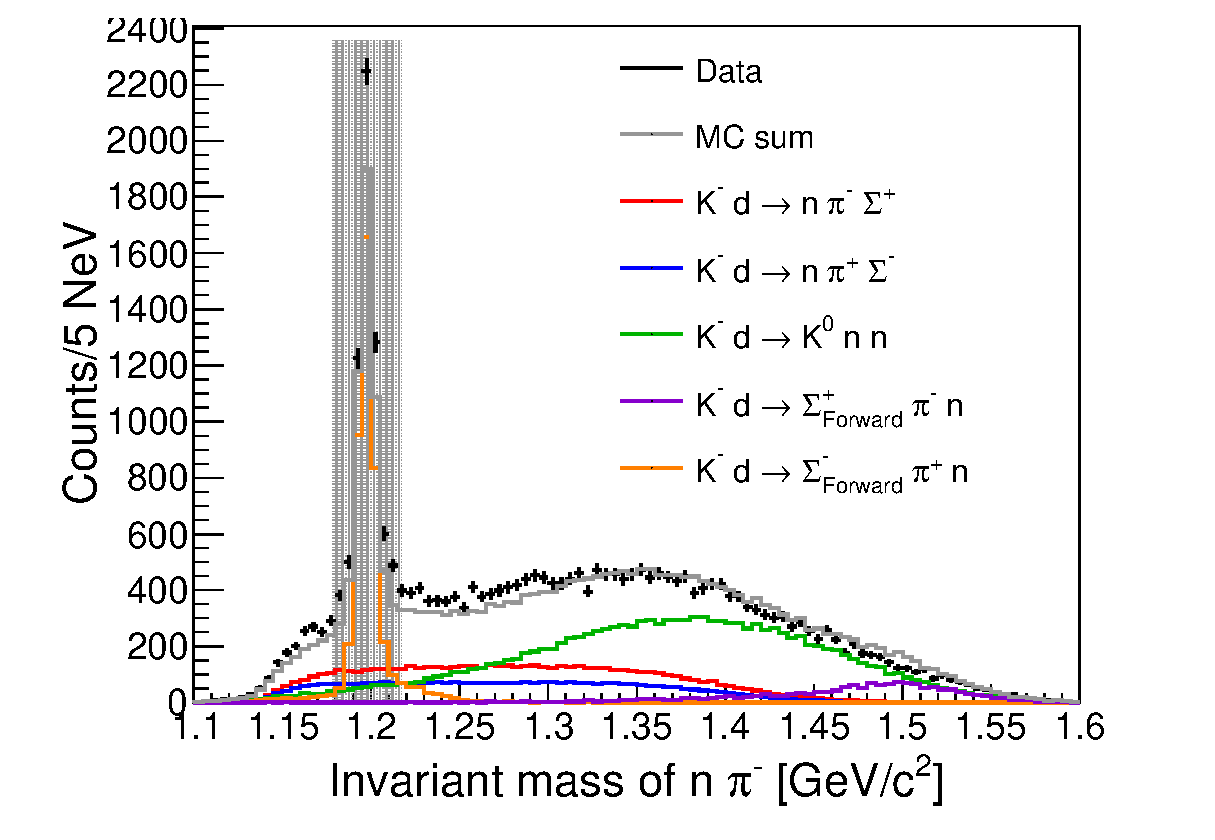
\includegraphics[width=4cm]{../pic/Dron/KN_ana/IM_npim.eps}
    \end{minipage}
    \begin{minipage}{0.33\hsize}
      \centering
      $n_{forward} \pi^-$ IM\\
      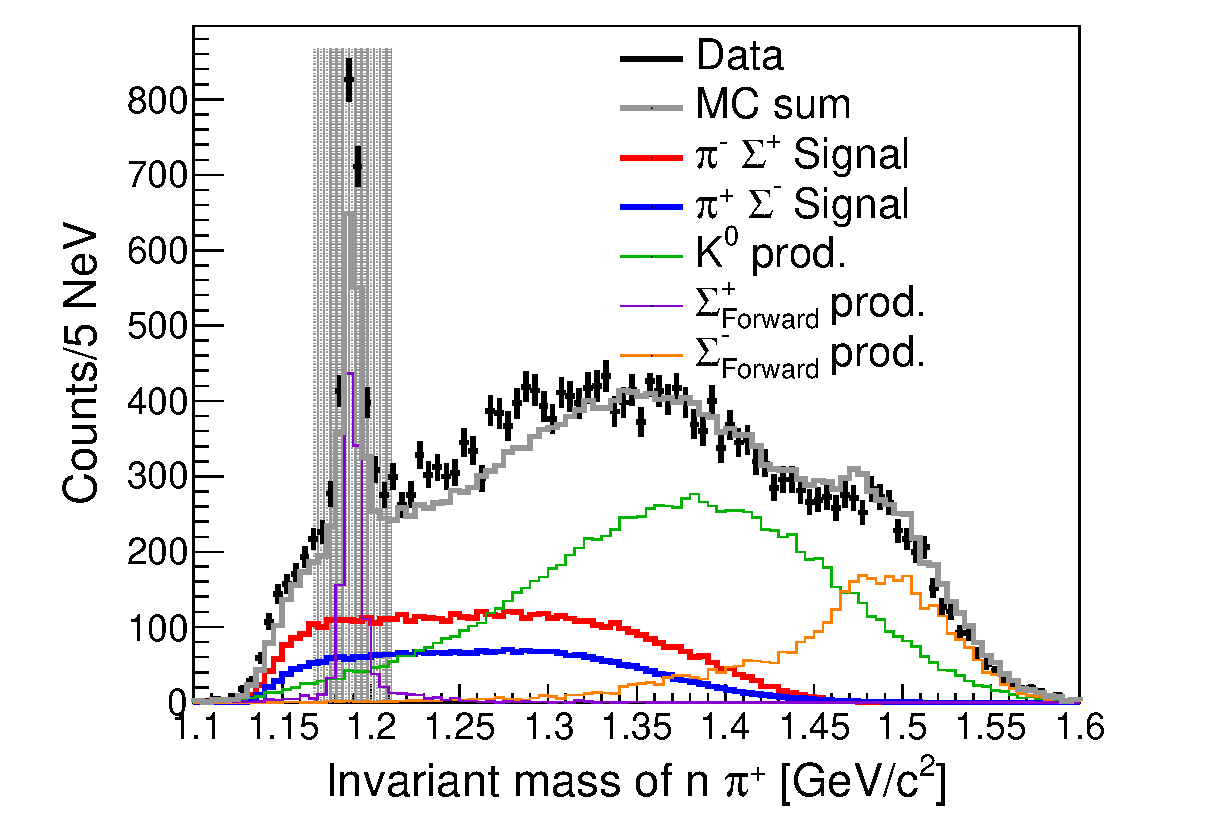
\includegraphics[width=4cm]{../pic/Dron/KN_ana/IM_npip.eps}
    \end{minipage}
  \end{tabular}
  \vspace{4mm}\\
  Each spectra are well reproduced. 
\end{frame}

\begin{figure}[htbp]
  \centering
  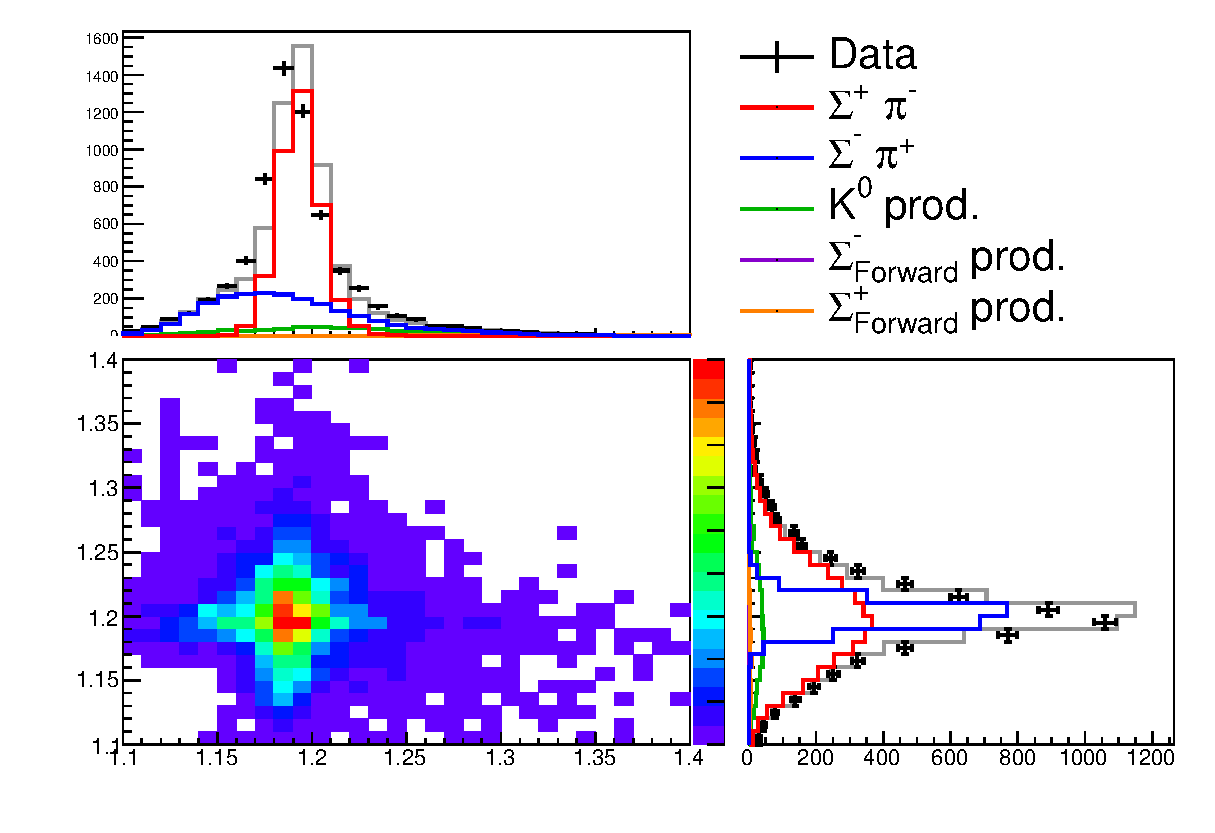
\includegraphics[width=12cm]{../pic/Run78/KN_ana_NC170_2sigma/KNpim_KNpip_MM.eps}
  \caption{
    This figure shows template fitting of the $d(K^-, n \pi)$ spectra to separate the $\pi^-\Sigma^+$ and $\pi^+ \Sigma^-$ modes.
    The lower left figure shows two-dimensional plots of $d(K^-, n \pi^-)$ and $d(K^-, n \pi^+)$ on the horizontal and vertical axes, respectively.
    The top and right panels show the projections onto each axis.
    The caption is the same as that of Figure.\ref{fig:fit_IM}.
  }
  \label{fig:fit_KNpi_MM_all}
\end{figure}


In this subsection, we explain procedure of template fitting, whose main purpose is decomposition of $\pi^- \Sigma^+$ and $\pi^+ \Sigma^-$ modes.
Template fitting is divided into two stages, one fitting to estimate the amount of background for $K^0$ and $\Sigma_{forward}$ production,
the other to separate $\pi^-\Sigma^+$ and $\pi^+\Sigma^-$ modes.
These fittings are performed using fitting with the likelihood method on a finite sample generated by Monte Carlo method\cite{temp_fit}.
There is no $\chi^2$ in this fitting,
but there is a value of $-2\log\Lambda$ that asymptotically approaches the $\chi^2$ when the number of samples become infinite, and the fitting is evaluated with this value.
Here, $\Lambda$ is the likelihood.

The first fitting is performed using the invariant mass distributions of $\pi^+ \pi^-$, $n \pi^+$ and $n \pi^-$ in the event that $K^-d \rightarrow n \pi^+ \pi^- n$ final state.
The $K^0$, $\Sigma^+$ and $\Sigma^-$ productions create peaks in the respective invariant mass distributions as shown in Fig.\ref{fig:fit_IM}.
The distributions reconstructed by fitting are also plotted in the same figure.
The bold line represents the case of backward $\pi \Sigma$ production of signal, with red and blue representing the $\pi^- \Sigma^+$ and $\pi^-\Sigma^+$ modes, respectively.
The other green, purple and orange lines represent the background for $K^0$, $\Sigma^-_{forward}$ and $\Sigma^+_{forward}$ production, respectively.
This fitting of $-2\log\Lambda$ is \IMfitChiSquare.
Degrees freedom is the number of bin with data, and $-2\log\Lambda/NDF \sim $\IMfitChiNDF. 
% For this purpose, the distribution is fitted with a Gaussian and a 5-th polynomial function, and the rejection region is defined by the 3$\sigma$ of the Gaussian.

\begin{figure}
  \begin{tabular}{ccccc}
    \begin{minipage}{0.2\hsize}
      \includegraphics[width=2.2cm]{../pic/Run78/KN_ana_NC170_2sigma/KNpi_MM_0.eps}
    \end{minipage}
    \begin{minipage}{0.2\hsize}
      \includegraphics[width=2.2cm]{../pic/Run78/KN_ana_NC170_2sigma/KNpi_MM_1.eps}
    \end{minipage}
    \begin{minipage}{0.2\hsize}
      \includegraphics[width=2.2cm]{../pic/Run78/KN_ana_NC170_2sigma/KNpi_MM_2.eps}
    \end{minipage}
    \begin{minipage}{0.2\hsize}
      \includegraphics[width=2.2cm]{../pic/Run78/KN_ana_NC170_2sigma/KNpi_MM_3.eps}
    \end{minipage}
    \begin{minipage}{0.2\hsize}
      \includegraphics[width=2.2cm]{../pic/Run78/KN_ana_NC170_2sigma/KNpi_MM_4.eps}
    \end{minipage}
  \end{tabular}
  \begin{tabular}{ccccc}
    \begin{minipage}{0.2\hsize}
      \includegraphics[width=2.2cm]{../pic/Run78/KN_ana_NC170_2sigma/KNpi_MM_5.eps}
    \end{minipage}
    \begin{minipage}{0.2\hsize}
      \includegraphics[width=2.2cm]{../pic/Run78/KN_ana_NC170_2sigma/KNpi_MM_6.eps}
    \end{minipage}
    \begin{minipage}{0.2\hsize}
      \includegraphics[width=2.2cm]{../pic/Run78/KN_ana_NC170_2sigma/KNpi_MM_7.eps}
    \end{minipage}
    \begin{minipage}{0.2\hsize}
      \includegraphics[width=2.2cm]{../pic/Run78/KN_ana_NC170_2sigma/KNpi_MM_8.eps}
    \end{minipage}
    \begin{minipage}{0.2\hsize}
      \includegraphics[width=2.2cm]{../pic/Run78/KN_ana_NC170_2sigma/KNpi_MM_9.eps}
    \end{minipage}
  \end{tabular}
  \begin{tabular}{ccccc}
    \begin{minipage}{0.2\hsize}
      \includegraphics[width=2.2cm]{../pic/Run78/KN_ana_NC170_2sigma/KNpi_MM_10.eps}
    \end{minipage}
    \begin{minipage}{0.2\hsize}
      \includegraphics[width=2.2cm]{../pic/Run78/KN_ana_NC170_2sigma/KNpi_MM_11.eps}
    \end{minipage}
    \begin{minipage}{0.2\hsize}
      \includegraphics[width=2.2cm]{../pic/Run78/KN_ana_NC170_2sigma/KNpi_MM_12.eps}
    \end{minipage}
    \begin{minipage}{0.2\hsize}
      \includegraphics[width=2.2cm]{../pic/Run78/KN_ana_NC170_2sigma/KNpi_MM_13.eps}
    \end{minipage}
    \begin{minipage}{0.2\hsize}
      \includegraphics[width=2.2cm]{../pic/Run78/KN_ana_NC170_2sigma/KNpi_MM_14.eps}
    \end{minipage}
  \end{tabular}
  \begin{tabular}{ccccc}
    \begin{minipage}{0.2\hsize}
      \includegraphics[width=2.2cm]{../pic/Run78/KN_ana_NC170_2sigma/KNpi_MM_15.eps}
    \end{minipage}
    \begin{minipage}{0.2\hsize}
      \includegraphics[width=2.2cm]{../pic/Run78/KN_ana_NC170_2sigma/KNpi_MM_16.eps}
    \end{minipage}
    \begin{minipage}{0.2\hsize}
      \includegraphics[width=2.2cm]{../pic/Run78/KN_ana_NC170_2sigma/KNpi_MM_17.eps}
    \end{minipage}
    \begin{minipage}{0.2\hsize}
      \includegraphics[width=2.2cm]{../pic/Run78/KN_ana_NC170_2sigma/KNpi_MM_18.eps}
    \end{minipage}
    \begin{minipage}{0.2\hsize}
      \includegraphics[width=2.2cm]{../pic/Run78/KN_ana_NC170_2sigma/KNpi_MM_19.eps}
    \end{minipage}
  \end{tabular}
  \begin{tabular}{ccccc}
    \begin{minipage}{0.2\hsize}
      \includegraphics[width=2.2cm]{../pic/Run78/KN_ana_NC170_2sigma/KNpi_MM_20.eps}
    \end{minipage}
    \begin{minipage}{0.2\hsize}
      \includegraphics[width=2.2cm]{../pic/Run78/KN_ana_NC170_2sigma/KNpi_MM_21.eps}
    \end{minipage}
    \begin{minipage}{0.2\hsize}
      \includegraphics[width=2.2cm]{../pic/Run78/KN_ana_NC170_2sigma/KNpi_MM_22.eps}
    \end{minipage}
    \begin{minipage}{0.2\hsize}
      \includegraphics[width=2.2cm]{../pic/Run78/KN_ana_NC170_2sigma/KNpi_MM_23.eps}
    \end{minipage}
    \begin{minipage}{0.2\hsize}
      \includegraphics[width=2.2cm]{../pic/Run78/KN_ana_NC170_2sigma/KNpi_MM_24.eps}
    \end{minipage}
  \end{tabular}
  \label{fig:fit_KNpi_MM}
  \caption{
    These figures are presented separately for each bin of $d(K^-, n)$ for fitting to separate $\pi^- \Sigma^+$ and $\pi^+ \Sigma^-$ modes.
    The top left figure shows the lowest missing mass in the $1.35$-$1.36$GeV bin, with the next bin represented as one goes to the right.
    In other words, one row is shown for the 0.05GeV region.
  }
\end{figure}

\begin{figure}[htbp]
  \centering

  \includegraphics[width=8cm]{../pic/Dron/tempFit_KNpi_MM_Chi2.eps}
  \caption{
    This figure shows the template fitting $-2\log\Lambda$ and $-2\log\Lambda/NDF$ for the separation of $\pi^- \Sigma^+$ and $\pi^+ \Sigma^-$ modes in each $d(K^-, n)$ bin.
    Black and red indicate $-2\log\Lambda$ and $-2\log\Lambda/NDF$, respectively.
    The horizontal axis is represented for $d(K^-, n)$ bins.
  }
  \label{fig:tempFit_KNpi_Chi2}
\end{figure}


The fitting to separate the $\pi^-\Sigma^+$ and $\pi^+\Sigma^-$ modes is performed for events from $K^-- d \rightarrow n \pi^+ \pi- n$, excluding $K^0 $and $\Sigma^{\pm}_{forward}$ production.
However, the background leakage is estimated by scaling the distribution reconstructed in the MC simulation by the intensity estimated by the invariant mass fitting.
This fitting is performed each bin of the missing mass of $d(K^-, n)$, since the scattering amplitude of $\bar{K}N \rightarrow \pi \Sigma$ depends on the $\pi \Sigma$ invariant mass.
For this fitting we use the $d(K^-, n \pi^-)$ and $d(K^-, n \pi^+)$ missing masses as shown in Fig.\ref{fig:fit_KNpi_MM_all}.
This figure shows the sum of the $d(K^- , n)$ bins.
The bottom left figure shows a two-dimensional figure of the $d(K^-, n \pi^-)$ and $d(K^-, n \pi^+)$ missing masses on the horizontal and vertical axes, respectively.
The top and right figures show the projections of the respective axes.
The missing mass of $d(K^-, n \pi)$ makes a peak at $\Sigma$ for the correct combination for the missing $\Sigma$, but is widely distributed in the kinematic region for the opposite charge.
For example, for $d(K^-, n \pi^-)$, the $\pi^- \Sigma^+$ mode has a peak structure as shown by the red line,
whereas the $\pi^+ \Sigma^-$ mode has a widely distributed structure as shown by the blue line.

Fig.\ref{fig:fit_KNpi_MM} shows the results for the fitting of each bin of $d(K^-, n)$ separately.
Fig.\ref{fig:tempFit_KNpi_Chi2} shows the $-2\log\Lambda$ and $-2\log\Lambda/NDF$ of this fitting in each $d(K^-, n)$ bin in black and red, respectively.

Fitting to estimate background and to separate $\pi^- \Sigma^+$ and $\pi^+ \Sigma^-$ modes cannot be performed simultaneously as they use different event samples.
They are therefore repeated in the following steps.

First, the separation of $\pi^- \Sigma^+$ and $\pi^+ \Sigma^-$ modes is performed without considering the background.
The obtained distribution of backward $\pi^{\mp} \Sigma^{\pm}$ modes is used for fitting to estimate the background,
which is then fed back into the fitting of the separation of $\pi^- \Sigma^+$ and $\pi^+ \Sigma^-$ modes.
After five iterations of this procedure, fitting is performed considering 2-step and direct $\Lambda(1520)$ generation for $K^0$ generation, which is described in the Appendix.\ref{apendix:K0_event}.
Finally, fitting of the separation of the $\pi^- \Sigma^+$ and $\pi^+ \Sigma^-$ modes is performed to obtain the final $\pi \Sigma$ spectrum as shown in Fig.\ref{fig:piS_num}..

\begin{figure}[htbp]
  \centering
  
  \includegraphics[width=8cm]{../pic/Dron/piS_num.eps}
  \caption{
    The $\pi^-\Sigma^+$ and $\pi^+\Sigma^-$ mode spectra obtained by template fitting are shown in arbitrary units.
    Red and blue lines indicate $\pi^-\Sigma^+$ and $\pi^+\Sigma^-$, respectively.
    The green vertical line is indicated the $\bar{K}N$ threshold.        
  }
  \label{fig:piS_num}
\end{figure}



%% \begin{frame}{Template fitting to decompose $K^0$ production}
  \begin{figure}
    \centering
    Invariant mass of $n K^0$\\
    \includegraphics[width=7.5cm]{../pic/Dron/K0_ana/npipi_IM_K0.eps}
  \end{figure}
  \centering
  2-step like component is seen about 11.5\%.\\
  Direct-$\Lambda(1520)$ prod. is seen about 7.7\%.\\
\end{frame}



\section{Conversion to the cross section}
\section{Conversion spectra to cross sections}
\begin{figure}[htbp]
  \centering
  \includegraphics[width=8cm]{../pic/Dron/KN_ana/kn_acc.eps}
  \caption{
    This figure shows the acceptance of $d(K^-, n)"\pi^{\mp}\Sigma^{\pm}"$.
    The red line indicates $\pi^- \Sigma^+$ and the blue line indicates $\pi^+ \Sigma^-$.
  }
  \label{fig:kn_acc}
\end{figure}

\begin{figure}[htbp]
  \centering
  \includegraphics[width=8cm]{../pic/Dron/KP_ana/kp_acc.eps}
  \caption{
    This figure shows $d(K^-, p)"\pi^-\Sigma^0"$ acceptance
  }
  \label{fig:kp_acc}
\end{figure}


This section describes the CDS acceptance correction.
For this correction, we use Monte Carlo simulation data for the $K^-d \rightarrow n \Lambda(1405)$, assuming a 2-step process,
which was also used for the template fitting in the previous section.
The CDS acceptance correction is applied not only to $d(K^-, n)\Lambda(1405)$ but also to $d(K^-, p)\Sigma^*$.
The simulation data for this correction were generated in the same way as for the $K^-d \rightarrow n \Lambda(1405)$ reaction.

The forward-going neutrons (protons) are generated with a slightly wider angular distribution (<8 degrees)
than the acceptance of the forward detector system.
However, since the purpose here is to estimate the CDS acceptance,
only the events that are detected by the forward detector are considered as the sample population.
Among these events, those that pass through the same analysis routine as the real data are regarded as valid events.
In the case of forward neutrons, the analysis includes events in which $\pi^+ \pi^-$ are detected,
followed by the selection of $d(K^-, n \pi^+ \pi^-)n$ events, and the rejection of $K^0$ and $\Sigma^{\pm}_{forward}$.
In the case of forward protons, valid events are those in which $\pi^- \pi^-$ are detected,
and are classified through the $d(K^-, p \pi^- \pi^-)\gamma p$ and $d(K^-, p \pi^-)\Lambda$ selections.

The CDS acceptances obtained for $d(K^-, n)\pi^{\mp}\Sigma^{\pm}$ and $d(K^-, p)\pi^-\Sigma^0$ are shown
in Figures \ref{fig:kn_acc} and \ref{fig:kp_acc}, respectively.



%% The acceptance of $d(K^-,n)"\pi^{\mp}\Sigma^{\pm}"$ and $d(K^-,p)"\pi^-\Sigma^0$ is corrected by MC simulations
%% in which nucleons are injected at a forward angle into the covered region of a forward detector with a uniform $\pi\Sigma$ mass distribution.
%% Since the solid angle of the forward detector is evaluated as subsection.\ref{subsec.XXX}, we adapt as the denominator the events for which the forward detector is analyzable.
%% The same analysis procedure as for the real data is applied to the MC simulation, and the final survival rate is evaluated and used as the acceptance.
%% That is, for $d(K^-, n)"\pi^{\mp}\Sigma^{\pm}"$, we apply $d(K^-, n \pi^+ \pi^-)"n"$ final state selection and rejection of $K^0$ and $\Sigma_{forward}$.
%% For $d(K^-, p)"\pi^-\Sigma^0"$, we apply the $d(K^-, p \pi^- \pi^-)"p \gamma"$ and $d(K^-, p \pi^-)"\Sigma^0"$ selections.
%% Fig.\ref{fig:kn_acc} shows the acceptance of $d(K^-, n)\pi^{\mp} \Sigma^{\pm}$.
%% Dents above the $\bar{K}N$ threshold are due to $K^0$ rejection.
%% The difference in absolute values between $\pi^- \Sigma^+$ and $\pi^+ \Sigma^-$ is due to the branching ratio of the $\Sigma$ decay.
%% Fig.\ref{fig:kp_acc} shows the acceptance of $d(K^-, p)"\pi^-\Sigma^0"$.

%% \begin{frame}{$K^0 cos\theta$ vs mom  {\bf Data}}
  \begin{tabular}{cc}
    \begin{minipage}{0.5\hsize}
      \begin{figure}
        Raw\\
        \includegraphics[width=6cm]{../pic/Run78/QE/K0_cos_mom_data.eps}
      \end{figure}
    \end{minipage}

    \begin{minipage}{0.5\hsize}
      \begin{figure}
        $Data(\cos_{K^0}, p_{K^0}))/A(\cos\theta_{K^0}, p_{K^0})$\\
%%        Accpectance corrected\\
        \includegraphics[width=6cm]{../pic/Run78/QE/K0_cos_mom_data_corr.eps}
      \end{figure}
    \end{minipage}
  \end{tabular}
  
  \centering

  Acceptance was presented at page.4
  
\end{frame}

%% \subsection{The spectrum of the $d(K^-, n)"n K^0"$}

\begin{figure}
  \centering
  \begin{tabular}{cc}
    \begin{minipage}{0.6\hsize}
      \includegraphics[width=7cm]{../pic/Run78/QE/KN_MM_wK0_tag.eps}
    \end{minipage}
    \begin{minipage}{0.4\hsize}
      \includegraphics[width=4cm]{../pic/Run78/QE/IM_pipi.eps}
    \end{minipage}
  \end{tabular}
  \caption{
    Right figure shows $K^0$ selection region and estimated background events which is zoom up of left figure of Fig\ref{fig:IM_fit}.
    Red lines indicate selection region.
    left figure shows $d(K^-, n)"n K^0"$ spectra with esmated backgrounds by MC template.
  }
  \label{fig:KN_MM_K0}
\end{figure}

Although the reaction can not measured below the $\bar{K}N$ threshold, 
in the $K^0$ take the strangeness, 
so these events are one of the strongest candidate of the prove for 1-step reaction strength of the $K^-N\rightarrow \bar{K}n$ reaction.\\
The backgrounds were estimated using the template fitting result which was shown in the right figure of Fit\ref{fig:KN_MM_K0}.
The background spectra shape of the $d(K^-, n)"n K^0"$ was indicated in the left figure of the same figure.
These spectra will be collected by the acceptance of the CDS using	the $K^0$ kinematics because detected particles by the CDS came from the $K^0$ decay.
The $K^0$ kinematics was represented as 2 variables function about the $\cos\theta$ and the absolute momentum value and
the acceptance of the CDS was collected event-by-event using the acceptance as weight function as the following equation.

\begin{equation}
  N_{corr}(m_{n K^0}) = \sum N(m_{n K^0}, \cos\theta_{K^0}, p_{K^0}) \cdot \frac{1}{A(\cos\theta_{K^0}, p_{K^0})} \label{eq:corr_K0} 
\end{equation}

\begin{figure}[htbp]
  \centering
  \includegraphics[width=7cm]{../pic/Run78/QE/K0_cos_mom_acc.eps}
  \caption{
    This figure shows the acceptance of the $K^-d\rightarrow K^0 n n$ reaction which was estimated by the Monte Calro simulation.
  }
  \label{fig:K0_acc}
\end{figure}

\begin{figure}[htbp]
  \centering
  \begin{tabular}{cc}
    \begin{minipage}{0.5\hsize}
      \includegraphics[width=7cm]{../pic/Run78/QE/K0_cos_mom_data.eps}
    \end{minipage}

    \begin{minipage}{0.5\hsize}
      \includegraphics[width=7cm]{../pic/Run78/QE/K0_cos_mom_BG.eps}
    \end{minipage}
  \end{tabular}
  \caption{
    These figure shows about $K^0$ emit angle and momentum in the experimental frame.
    Left figure shows about data and right figure shows background estimated by the Monte Calro.
  }
  \label{fig:K0_cos_mom}
\end{figure}

For this collection, the acceptance was estimated using the $K^- d \rightarrow n_{forwad} (K^0 n)$ reaction.
The mass of the $n K^0$ was generated flat distribution from the $K^0 n$ mass threshold to the kinematical threshold
to accumulate widely and isotropically acceptance which was shown in Fig\ref{fig:K0_acc}
This acceptance collection was adopted to the signal and the backgrounds.
Fig\ref{fig:K0_cos_mom} shows the $K^0$ kinmatics distribution about the data and the backgrounds estimated by the MC sim.
By this operation, we obtained the acceptance collected spectra as shown in Fig\ref{fig:KN_MM_K0_corr}.
Because the data distribution located at the edge of the acceptance and the backgrounds widely distributed, in the acceptance corrected spectra, the signal was enhanced.

\begin{figure}[htbp]
  \centering
  \includegraphics[width=8cm]{../pic/Run78/QE/K0_spec_wBG.eps}
  \caption{
    This figure shows acceptance corrected spectrum of the $d(K^-, n)"n K^0"$.
    Black line indicates data and color plots indicate the background reproduced by the Monte Calro simulation.
  }
  \label{fig:KN_MM_K0_corr}
\end{figure}


%% For $K^0$ production events, we use acceptance for $K^0$ kinematics because all detected particles are of $K^0$ origin.
%% We estimate the two-dimensional acceptances for $K^0$ momentum and $K^0$ scattering angles as shown in Fig\ref{fig.K0_cos_mom_acc}, and weight each event to correct for acceptances.
%% Fig.\ref{fig:K0_spec} shows acceptance corrected spectra of $K^0$ production with reproduced BG by MC simulations.
%% It can be seen that the data are concentrated in the backward and high momentum regions where the acceptances are small,
%% while the MC is distributed over the whole region as shown in Fig.\ref{fig:K0_cos_mom}.
%% In other words, the acceptance correction suppresses BG and emphasizes true $K^0$ production.

\subsection{$d(K^-, n)$ scaling factor}
$d(K^-, n)"X"$ spectrum can be converted from counts to the differential cross section ($\frac{d^2\sigma}{d\Omega dm}$) excepting the acceptance of the the CDS that is depend on the reaction.
The parameters was used for the conversion were summarized in Table\ref{tab:KN_scale}.

First one is luminosity which was consist of number of target, number of irradiated kaon, DAQ live rate, trigger efficeincy.
The number of target was defined from length of fiducial volume ($10cm$) and target density which was evaluated from measured tempature.
The number of irradiated kaon was defined by correcting kaon number counted up by the scaler DAQ by ratio of true kaon in kaon trigger which was described in Sec\ref{sec:beam_line_ana}.
About DAQ live rate and trigger efficiency were discribed in Sec\ref{sec:trigger}.
The luminosity was evaluated run-by-run.
In the table, these items were represented value weighted by data statistics as typical value.

Next is about the CDS which was CDC efficiency discribed in Sec\ref{sec:CDC_eff}.
Accpectances of CDS were estimated and corrected by the Monte Carlo simulation data.
These evaluations were described in individual section for each reactions.

Last one is about the NC which was consists of acceptance and efficiency.
The efficiency of the NC was further decomposed to intrinsic one and overveto by the CVC and the BVC that was described in Sec\ref{sec:NC_eff}.
The acceptance of the NC was estimated from the NC position and the error was evaluated from difference of the first layer and the last layer of the NC.

\input{analysis/KN_scaling_table}


\begin{table}
  \caption{
    Summary table of $d(K^-, p)$ scaling parameters
  }

  \hspace{-2cm}
  \begin{tabular}{cc|cc|cc}
    \multicolumn{2}{c|}{Component}  & value            & error           & value  & error \\
    \hline
    \hline
    Luminosity   ($/\mu b$)    &    & 2478             & 81          &  & \\
    & Target Length (cm)       &  & & 10               &                  \\
    & Target density $[g/cm^3]$&  & & 0.1624           & 0.0014           \\
    & Number of Kaon           &  & & 2.05$\times 10^{10}$ &              \\
    & Survival ratio of $K^-$  &  & & 0.336            & 0.0001           \\
    & DAQ live ratio           &  & & 0.821            & 0.0001           \\
    \multicolumn{2}{c|}{Trigger efficiency}  &  & &                  &    \\
    \hline
    & $K \otimes$CDH1          &  & & 0.9527           & 0.0003 \\
    & Charge                   &  & & 0.9559           & 0.0004 \\
    \hline
    \hline
    Efficiency of the CDC      &    & 0.977            & 0.04    &  & \\
    \hline
    %% \hline
    %% Acceptance of the PC/CVC (msr) & & \multicolumn{4}{|c}{Evaluate by the SIM} \\
    \hline
    Efficeincy of the forward detectors  &    & 0.819            & 0.042   &  & \\
    Efficeincy of the FDC1               &    & 0.987            & 0.005   &  & \\
  \end{tabular}
  \label{table:KP_scaling}
\end{table}


\begin{figure}[htbp]
  \centering
  \includegraphics[width=8cm]{../pic/Run78/KP_ana/solid_ang_144.eps}
  \caption{
    This figure shows the effective rates of solid angle elements in the 1.44–1.45 GeV $\pi^-\Sigma^0$ mass bin,
    as estimated by Monte Carlo simulations.
  }
  \label{fig:PCCVC_SA_elem}
\end{figure}

\begin{figure}[htbp]
  \centering
  \includegraphics[width=8cm]{../pic/Dron/PCCVC_SA.eps}
  \caption{
    This figure shows the relationship between the mass of the $\pi^-\Sigma^0$ system and
    the solid angles of the forward detectors (FDC1 and PC/CVC) with respect to the outgoing forward proton.
    The red line indicates the solid angle of the NC detector with respect to the forward neutron.
  }
  \label{fig:PCCVC_SA}
\end{figure}


The factors for converting to double-differential cross sections are explained here.
These can be categorized into the following three components:
\begin{enumerate}
\item Luminosity, which is determined by the number of incident beam particles and the number of target nuclei;
\item The solid angle and detection efficiency of the forward-scattered neutrons (or protons) produced in the reaction;
\item The detection efficiency of detectors.
\end{enumerate}

These are summarized in Tables \ref{table:KN_scaling} and \ref{table:KP_scaling} for the forward neutron and forward proton cases, respectively.

Luminosity is a quantity that represents the product of the number of incident beam particles and the number of target particles.
The beam intensity is evaluated by multiplying the beam scaler counts by the DAQ live ratio,
described in Section \ref{sec:DAQ_eff}, which accounts for the fraction of data actually recorded for analysis;
the trigger efficiency, described in Section \ref{sec:trig_eff}, which accounts for whether a trigger signal was actually generated;
and the fraction of $K^-$ beam triggers that passed through the fiducial volume of the target, as described in Section \ref{sec:beam_ana}.
This beam-related quantity is calculated and summed on a run-by-run basis.
Tables \ref{table:KN_scaling} and \ref{table:KP_scaling} show representative values
consisting of the average over all runs and the errors evaluated from the fluctuations.
For the number of target particles, the density of the liquid deuterium target is estimated from the monitored temperatures,
as described in Section \ref{sec:target} The uncertainty is evaluated based on fluctuations during the production run and
is calculated by multiplying the density by the length of the fiducial volume.

% The temperature of the liquid deuterium target is monitored, as described in Section \ref{sec:target},
% and this value is used to evaluate its density.

In the case of forward neutrons, since they travel in straight trajectories,
the solid angle can be defined by the area covered by the NC. When the solid angle is evaluated at the center of the NC
and the variation is assessed by shifting the evaluation point front and back, it is determined to be 21.5 $\pm$ 0.2 [msr]\%.
The detection efficiency of the neutron detector can be divided into two components
the intrinsic detection efficiency of the NC for neutrons and the over-veto effect by the CVC.
The intrinsic neutron detection efficiency is evaluated to be 31.7 $\pm$ 1.6 [\%] using the reaction
$K^- p \rightarrow K^0 n \rightarrow \pi^+ \pi^- n$ with a liquid hydrogen target, as described in Section \ref{sec:NC_eff}.
The over-veto effect in the CVC, which is also considered to be strongly influenced by beam-induced background,
is evaluated to be 8.1 $\pm$ 0.7 [\%] using the production run data, also described in Section \ref{sec:NC_overveto}.

In the case of forward protons, since they are bent by the Usniwaka magnet,
the solid angle coverage depends on the momentum of the forward-scattered proton, i.e., the mass of the $\pi^-\Sigma^0$ system.
To estimate this, we use a dataset similar to the Monte Carlo simulation used for the acceptance correction.
The solid angle for a given $\pi^-\Sigma^0$ mass region is evaluated by dividing the angular space into small solid angle elements.
For each element,
the detection efficiency of the forward detector system (CVC/PC) is evaluated based on whether the proton can actually be detected.
The effective solid angle for each element is then calculated by multiplying the element's solid angle by its detection efficiency,
as shown in Figure \ref{fig:PCCVC_SA_elem}
Finally, the total solid angle is obtained by summing these effective solid angles over all elements, as shown in Figure \ref{fig:PCCVC_SA}.
The solid angle does not change significantly in the region of interest.

In this data set, hadronic reactions and similar processes that could cause secondary interactions are turned off
to avoid double-counting losses already accounted for in the detection efficiency of forward protons evaluated in Section \ref{sec:PC_eff}.
Here, the detection efficiency of protons was estimated to be 81.9 $\pm$ 4.2 [\%] using the $K^- d \rightarrow \pi^- \pi^- p p$ reaction.
Also,
the detection efficiency of FDC1 was evaluated to be 98.7 $\pm$ 0.5 [\%] using the BVC as the trigger detector under the pion beam conditions,
as described in Section \ref{sec:FDC1_eff}.

After applying the CDS acceptance obtained in the previous subsection and the correction factors described here,
we obtain the $d(K^-, n)\pi^{\mp}\Sigma^{\pm}$ and $d(K^-, p)\pi^-\Sigma^0$ cross sections,
as shown in Figures \ref{fig:Charge_CS} and \ref{fig:pimS0_CS}, respectively.

% \begin{frame}{Cross Section of $d(K^-, n)"n K^0"$}
  \begin{figure}
    \includegraphics[width=8cm]{../pic/Run78/QE/K0_CS.eps}
  \end{figure}
  \centering
  Box indicates staticial errors.
%%  BG was subtracted.
\end{frame}

\begin{figure}[htbp]
  \centering
  \includegraphics[width=9cm]{../pic/Dron/KN_ana/ChargeCS.eps}
  \caption{
    The red figure and blue figure shows about $d(K^-, n)"\pi^+\Sigma^-"$ and $d(K^-, n)"\pi^-\Sigma^+"$, respectively.
    The inner frame (thin line), outer frame (thick line), and error bars represent the addition of statistical errors, fitting errors, and conversion errors, which were calculated by root-mean-square.
    The green vertical lines indicates $\bar{K}N$ threshold.
  }
  \label{fig:Charge_CS}
\end{figure}

\begin{figure}[htbp]
  \centering
  \includegraphics[width=9cm]{../pic/Dron/KP_ana/pimS0_CS.eps}
  \caption{
    This figure shows the cross section of $d(K^-, p)"\pi^- \Sigma^0"$.
    The box represents the statistical error, and the error bar represents the root mean squares of the conversion factor added to it.
    The green vertical lines indicates $\bar{K}N$ threshold.
  }
  \label{fig:pimS0_CS}
\end{figure}










%% The solid angle for a given $\pi^-\Sigma^0$ mass region is evaluated by summing the effective solid angles,
%% each weighted by the detection efficiency of the forward detector system (CVC/PC), over the solid angle bins of the generated protons.

%% In this data set, hadron reactions and other reactions are turned off to prevent double-counting of losses due to reactions included in the detection efficiency of forward protons evaluated in Section 2.3.


%% The obtained spectra are converted to cross sections.
%% For this purpose, the target, beam, and DAQ efficiencies are summarized as luminosity.
%% The target and beam quantities are discussed in Sections.\ref{sec:target} and \ref{sec:Kbeam}, respectively.
%% The DAQ efficiency consists of two parts, one of which is the DAQ live rate and the other is the trigger efficiency, described in Sections.\ref{sec:DAQ_live_rate} and \ref{sec:trigger}.
%% Detector efficiency is also evaluated and corrected for conversion to cross sections.
%% The CDC, NC, and PC efficiencies are described in Sections.\ref{sec:CDC}, \ref{sec:NC}, and \ref{sec:PC}, respectively. 
%% These conversion factors are common for the $\pi \Sigma$ spectra.
%% These factors are summarized in Table.\ref{table:KN_scaling} and Table.\ref{table:KP_scaling} about $d(K^-, n)$ and $d(K^-, p)$, respectively.

%% On the other hand, the acceptances depend on the $\pi \Sigma$ mass spectra.
%% % In the case of $d(K^-, n)"\pi^{\mp} \Sigma^{\pm}"$, the separation ratio of $\pi^- \Sigma^+$ and $\pi^+ \Sigma^-$ is also depend on.
%% We obtain the cross section of $d(K^-, n)"n K^0"$, $d(K-, n)"\pi^-\Sigma^0"$ and $d(K^-, p)"\pi^- \Sigma^0"$ by adapting the these corrections,
%% which are shown in Figure.\ref{fig:nK0_CS}, Figure.\ref{fig:Charge_CS}, and Figure.\ref{fig:pimS0_CS}, respectively.
%% We obtain the cross section of $d(K-, n)"\pi^-\Sigma^0"$ and $d(K^-, p)"\pi^- \Sigma^0"$ by adapting the these corrections,
%% which are shown in Fig.\ref{fig:Charge_CS}, and Fig.\ref{fig:pimS0_CS}, respectively.

% \begin{figure}[htbp]
  \centering
  \includegraphics[width=6cm]{../pic/Dron/K0_ana/K0_CS.eps}
  \caption{
    This figure shows the cross section of $d(K^-, n)"n K^0"$.
    The box represents the statistical error, and the error bar represents the root mean squares of the conversion factor added to it.
    The green vertical lines indicates $\bar{K}N$ threshold.
  }
  \label{fig:nK0_CS}
\end{figure}

\begin{figure}[htbp]
  \centering
  \includegraphics[width=6cm]{../pic/Dron/KN_ana/ChargeCS.eps}
  \caption{
    The red figure and blue figure shows about $d(K^-, n)"\pi^+\Sigma^-"$ and $d(K^-, n)"\pi^-\Sigma^+"$, respectively.
    The inner frame (thin line), outer frame (thick line), and error bars represent the addition of statistical errors, fitting errors, and conversion errors, which were calculated by root-mean-square.
    The green vertical lines indicates $\bar{K}N$ threshold.
  }
  \label{fig:ChargeCS}
\end{figure}

\begin{figure}[htbp]
  \centering
  \includegraphics[width=6cm]{../pic/Dron/KP_ana/pimS0_CS.eps}
  \caption{
    This figure shows the cross section of $d(K^-, p)"\pi^- \Sigma^0"$.
    The box represents the statistical error, and the error bar represents the root mean squares of the conversion factor added to it.
    The green vertical lines indicates $\bar{K}N$ threshold.
  }
  \label{fig:pimS0_CS}
\end{figure}


% We discuss the physical mean about obtained spectra.






\section{Spectra}
\subsection{Qualitative properties of obtained spectra}
\begin{figure}[htbp]
  \centering
  \includegraphics[width=8cm]{../pic/Dron/All_CS.eps}
  \caption{
    The obtained cross sections are plotted simultaneously in this figure.
    The $d(K^-, n)"\pi^-\Sigma^+$, $d(K^-, n)"\pi^+\Sigma^-"$, $d(K^-, n)"n K^0"$, and $d(K^-, p)"\pi^- \Sigma^0"$ plot as red, blue, green, and orange, lines respectively.
    The $d(K^-, n)"n K^0"$ is scaled to 1/10.
    The green virtical line indicates the $\bar{K}N$ threshold.
  }
  \label{fig:all_CS}
\end{figure}


The $d(K^-, n)\pi^{\mp}\Sigma^{\pm}$ and $d(K^-, p)\pi^-\Sigma^0$ spectra obtained through the procedures described in the previous section
are shown together in Figure \ref{fig:all_CS}.
In this figure, the green vertical line indicates the $\bar{K}N$ threshold.
This section discusses the qualitative features of the obtained spectra.

The experiment is interpreted as a two-step reaction, as described in Section \ref{sec:E31}.
The $\pi^-\Sigma^0$ spectrum contains only the $I=1$ component from the second-step scattering,
and this second-step scattering does not exhibit a significant structure, as there is no pole near the $\bar{K}N$ threshold.
As a result, the $\bar{K}N$ spectrum reflects the first-step scattering more directly.
A bump-like shape emerges from the $\bar{K}N$ threshold due to the Fermi motion of the spectator.

For the $I=0$ component, the second-step scattering is expected to exhibit a pronounced structure below the $\bar{K}N$ threshold
due to the presence of poles in that region.
This results in a spectral shape with a stronger enhancement below the $\bar{K}N$ threshold compared to the bump-like feature originating
from the first-step scattering.
Indeed, the observed $\pi^{\mp}\Sigma^{\pm}$ spectra, which contain both $I=0$ and $I=1$ components as well as their interference,
exhibit a clear structure below the $\bar{K}N$ threshold.
The overall spectral intensity is also larger than that of the $\pi^-\Sigma^0$ spectrum,
which only contains the $I=1$ component, due to the pole contribution in the $I=0$ channel.
The interference between the $I=0$ and $I=1$ components appears as a difference between the $\pi^-\Sigma^+$ and $\pi^+\Sigma^-$ spectra.
Since the measured spectra show a clear asymmetry between them,
the interference effect between $I=0$ and $I=1$ was observed in the reactions in this experiment.

In the second-step scattering near the $\bar{K}N$ threshold,
$S$-waves are expected to dominate due to the small angular momentum transfer transfer.
However, it is well known that in this region there are $I=0$ $D$-wave resonances, such as the $\Lambda(1520)$,
and $I=1$ $P$-wave resonances, such as the $\Sigma(1385)$.
The absence of structures around the $\Sigma(1385)$ region in the measured $I=1$ $\pi^-\Sigma^0$ spectrum,
as well as around both the $\Sigma(1385)$ and $\Lambda(1520)$ regions in the $\pi^+\Sigma^-$ and $\pi^-\Sigma^+$ spectra
with mixed $I=0$ and $I=1$ contributions, confirms that the $S$-wave dominates in the reactions observed in this experiment.


\subsection{Comparison with theoritical calculations}
\input{discussion/spectra/comp_theoritical_cacl}
\subsection{$\bar{K}N$ Pole parameters assuming the 2-step reaction}
Next, we discuss the method for obtaining the $\bar{K}N$ pole parameters through fitting under the assumption of a 2-step reaction.
This approach is similar to that used by Noumi et el., as introduced in Chapter 1.
Since this analysis method focuses only on $I=0$, the obtained spectra are separated into components of $I=0$.
In this procedure, the spectra are further separated into components of $I=1$ and, in addition, the interference term between $I=0$ and $I=1$.
The obtained spectrum can be expressed as follows from the isospin relation.

\newcommand{\Tmat}{T_{\bar{K}N \rightarrow \pi \Sigma}}
\newcommand{\Cfirst}{C_{K^- N \rightarrow \bar{K}N}}
\newcommand{\CS}{\frac{d\sigma}{d\Omega dM}}
\begin{align}
  \CS(\pi^\mp \Sigma^\pm) \propto & \left| \Cfirst^0 \Tmat^{I=0} \mp \Cfirst^1 \Tmat^{I=1} \right|^2 \nonumber \\
  = & \left| \Cfirst^0 \Tmat^{I=0} \right|^2 + \left| \Cfirst^1 \Tmat^{I=1} \right|^2 \nonumber \\
    & \mp 2\mbox{Re}( \Cfirst^0 \Cfirst^1 \Tmat^{I=0} \Tmat^{I=1} ) & \label{eq:Charge_piS} \\
  \CS(\pi^- \Sigma^0) \propto & \left| \Cfirst^1 \Tmat^{I=1} \right|^2 \label{eq:pimS0}
\end{align}

Here, $\Tmat^{I=0,1}$ represents the $T$ matrix of the second $\bar{K}N \rightarrow \pi \Sigma$ scattering for isospin $I=0$ and $I=1$.
Additionally, $\Cfirst^{0,1}$ denotes the factor for the first $K^- p \rightarrow \bar{K}N$ scattering,
corresponding to the isospin $I=0$ and $I=1$ components of the second scattering.

Since it can be expressed as shown in Equation (\ref{eq:Charge_piS}), (\ref{eq:pimS0}),
the spectra corresponding to $I=0$, $I=1$, and their interference terms can be written as follows.
\begin{align}
  & \CS(I=0) \propto \frac{1}{2}\left( \CS(\pi^- \Sigma^+)+\CS(\pi^+ \Sigma^-)-\CS(\pi^-\Sigma^0) \right) \label{eq:I0}\\
  & \CS(I=1) \propto \CS(\pi^- \Sigma^0) \label{eq:I1}\\ 
  & \CS(int) \propto \left( \CS(\pi^- \Sigma^+)-\CS(\pi^+\Sigma^+) \right) \label{eq:interfer}
\end{align}

\begin{figure}[htbp]
  \centering
  \begin{tabular}{ccc}
    \begin{minipage}{0.33\hsize}
      \includegraphics[width=4cm]{../pic/Dron/fit_I0_KzeroN.eps}
    \end{minipage}
    \begin{minipage}{0.33\hsize}
      \includegraphics[width=4cm]{../pic/Dron/fit_I0_KN.eps}
    \end{minipage}
    \begin{minipage}{0.33\hsize}
      \includegraphics[width=4cm]{../pic/Dron/fit_I0_Kmp.eps}
    \end{minipage}
  \end{tabular}
  \begin{tabular}{ccc}
    \begin{minipage}{0.33\hsize}
      \includegraphics[width=4cm]{../pic/Dron/fit_scat_amp_I0_KzeroN.eps}
    \end{minipage}
    \begin{minipage}{0.33\hsize}
      \includegraphics[width=4cm]{../pic/Dron/fit_scat_amp_I0_KN.eps}
    \end{minipage}
    \begin{minipage}{0.33\hsize}
      \includegraphics[width=4cm]{../pic/Dron/fit_scat_amp_I0_Kmp.eps}
    \end{minipage}
  \end{tabular}
  \caption{
    This figure shows the $I=0$ spectrum obtained from Eq. (\ref{eq:I0}) and the fit results assuming a 2-step reaction.
    In the upper panel, the error bars represent the experimental data, the red line indicates the spectrum resulting from the fit,
    the solid line corresponds to the spectrum convolved with detector resolution, and the dashed line represents the spectrum without resolution.
    The lower panel displays the scattering amplitude for the two-step $\bar{K}N \rightarrow \bar{K}N$ scattering,
    where the red line indicates the real part and the blue line shows the imaginary part.
    The lines are the best-fit values and the bands hatched in color represent the width of the error due to fitting.
  }
  \label{fig:fit_2step_I0}
\end{figure}


The 2-step response can be expressed as follows,
\begin{equation*}
   \frac{d\sigma}{dM_{\pi\Sigma}d\Omega_{n}}
   =\left| \bra{n_{\theta=0}\pi\Sigma} T^2_{\bar{K}N_2 \rightarrow \pi \Sigma}
   G_0(\bar{K}, N_2) T^1_{K^-N_1 \rightarrow \bar{K} N} \ket{K^-\Phi_{d}} \right|^2 
\end{equation*}
where $G_0(\bar{K}, N_2)$, represents the Green's function describing the propagation of virtual $\bar{K}$ mesons
between the first and second scattering steps.
This equation can be factorized using the deuterium wavefunction $\psi_d(p)$ and decomposed into
a 1-step response $f_{res}(M_{\pi \Sigma})$function and a 2-step scattering amplitude as shown below.
\begin{align*}
   & \frac{d\sigma}{dM_{\pi\Sigma}d\Omega_{n}}
     \sim \left| T^2_{\bar{K}N_2 \rightarrow \pi \Sigma} \right|^2 F_{res}(M_{\pi \Sigma}) \\
   & F_{res}(M_{\pi \Sigma}) = \left| \int G_0(\bar{K}, N_2) T^1_{K^-N\rightarrow \bar{K}N} \psi_d(p) d^3p_{N} \right|^2
\end{align*}
The $T$-matrix of the second scattering is expressed as follows, utilizing the low-energy expansion up to the second order for the two channels
\cite{Lensniak}.
\begin{align*}
   & T^2_{\bar{K} N \rightarrow \bar{K}N} = \frac{A}{1-iA k_2+\frac{1}{2}A Rk_2^2}\\
   & T^2_{\bar{K} N \rightarrow \pi \Sigma} =
   \frac{e^{i\delta}}{\sqrt{k_1}}\frac{\sqrt{{\bf Im}A-\frac{1}{2}|A|^2{\bf Im}Rk_2^2}}{1-iAk_2+\frac{1}{2}ARk_2^2}
\end{align*}

This fit includes the scattering length $A$ and the effective range $R$ of the second-step scattering,
along with a parameter determining the overall scale.
In other words, the shape of the first-step scattering (reaction function) is fixed,
and the spectrum shape is determined solely by the second-step scattering.
The scattering length and effective range are complex numbers, so there are five free parameters in total.
This fitting is performed using three $\bar{K}N$ threshold values: $K^- p$, $\bar{K}N$ (the average of $K^- p$ and $K^0 n$), and $K^0 n$.
The discrepancies in the results arising from the differences in threshold values are evaluated as a source of systematic error.
These differences in threshold values are reflected not only in the mass of the $\bar{K}N$ channel in the $T$-matrix of the seccond-scattering
but also in the mass of the nucleon used to calculate the response function in the first-step scattering.
The figure above shows the results of the fit: black error bars represent the data,
and the red solid line shows the fit results convolved with detector resolution, which are used to calculate the chi-square.
The red dashed line shows the fit spectrum without detector resolution,
and the blue dashed line indicates the response function, scaled arbitrarily.
The figure below shows the scattering amplitude obtained from the fit, with red and blue representing the real and imaginary parts, respectively.
The lines indicate the best-fit result, and the bands show the error range,
determined by the maximum and minimum values when adjusting the real and imaginary parts of $A$ and $R$ within their error margins.
The central values of the parameters and the fitting errors were evaluated in terms of the average $\bar{K}N$ threshold,
with $A = \fitScatLength$ and $R = \fitEffRange$.
These values need to be converted to the pole’s position [MeV] and width [MeV],
where the pole is defined by setting the denominator of the $T$-matrix to zero, i.e., by solving the following equation.
\begin{equation}
\frac{1}{2}ARk^2+Ak^2+1=0 \label{eq:pole}
\end{equation}
Where $k$ is the momentum of the $\bar{K}N$ center-of-mass system, converted to mass by $m=\sqrt{m_{\bar{K}N}^2+k^2}$.

\begin{figure}
  \begin{tabular}{ccc}
    \begin{minipage}{0.33\hsize}
      \includegraphics[width=4cm]{../pic/Dron/fit_L1405_pole_Kmp_5.eps}
    \end{minipage}
    \begin{minipage}{0.33\hsize}
      \includegraphics[width=4cm]{../pic/Dron/fit_L1405_pole_KN_5.eps}
    \end{minipage}
    \begin{minipage}{0.33\hsize}
      \includegraphics[width=4cm]{../pic/Dron/fit_L1405_pole_KzeroN_5.eps}
    \end{minipage}
  \end{tabular}

  \begin{tabular}{ccc}
    \begin{minipage}{0.33\hsize}
      \includegraphics[width=4cm]{../pic/Dron/fit_L1405_pole_Kmp_4.eps}
    \end{minipage}
    \begin{minipage}{0.33\hsize}
      \includegraphics[width=4cm]{../pic/Dron/fit_L1405_pole_KN_4.eps}
    \end{minipage}
    \begin{minipage}{0.33\hsize}
      \includegraphics[width=4cm]{../pic/Dron/fit_L1405_pole_KzeroN_4.eps}
    \end{minipage}
  \end{tabular}

  \begin{tabular}{ccc}
    \begin{minipage}{0.33\hsize}
      \includegraphics[width=4cm]{../pic/Dron/fit_L1405_pole_Kmp_3.eps}
    \end{minipage}
    \begin{minipage}{0.33\hsize}
      \includegraphics[width=4cm]{../pic/Dron/fit_L1405_pole_KN_3.eps}
    \end{minipage}
    \begin{minipage}{0.33\hsize}
      \includegraphics[width=4cm]{../pic/Dron/fit_L1405_pole_KzeroN_3.eps}
    \end{minipage}
  \end{tabular}

  \begin{tabular}{ccc}
    \begin{minipage}{0.33\hsize}
      \includegraphics[width=4cm]{../pic/Dron/fit_L1405_pole_Kmp_2.eps}
    \end{minipage}
    \begin{minipage}{0.33\hsize}
      \includegraphics[width=4cm]{../pic/Dron/fit_L1405_pole_KN_2.eps}
    \end{minipage}
    \begin{minipage}{0.33\hsize}
      \includegraphics[width=4cm]{../pic/Dron/fit_L1405_pole_KzeroN_2.eps}
    \end{minipage}
  \end{tabular}

  \begin{tabular}{ccc}
    \begin{minipage}{0.33\hsize}
      \includegraphics[width=4cm]{../pic/Dron/fit_L1405_pole_Kmp_1.eps}
    \end{minipage}
    \begin{minipage}{0.33\hsize}
      \includegraphics[width=4cm]{../pic/Dron/fit_L1405_pole_KN_1.eps}
    \end{minipage}
    \begin{minipage}{0.33\hsize}
      \includegraphics[width=4cm]{../pic/Dron/fit_L1405_pole_KzeroN_1.eps}
    \end{minipage}
  \end{tabular}
  
  \begin{tabular}{ccc}
    \begin{minipage}{0.33\hsize}
      \includegraphics[width=4cm]{../pic/Dron/fit_L1405_pole_Kmp_0.eps}
    \end{minipage}
    \begin{minipage}{0.33\hsize}
      \includegraphics[width=4cm]{../pic/Dron/fit_L1405_pole_KN_0.eps}
    \end{minipage}
    \begin{minipage}{0.33\hsize}
      \includegraphics[width=4cm]{../pic/Dron/fit_L1405_pole_KzeroN_0.eps}
    \end{minipage}
  \end{tabular}
  
  \caption{
    This figure shows the distribution and fit of the poles of $\Lambda(1405)$, generated using Gaussian random numbers.
    The right, center, and left panels correspond to the results based on the $K^- p$, $\bar{K}N$, and $K^0 n$ thresholds, respectively.
    The top row represents the fit over the entire range,
    followed by rows corresponding to the equivalent ranges of $3\sigma$, $2.5\sigma$, $2\sigma$, $1.5\sigma$, and $1\sigma$.
    The fit results are shown as red lines, with gray hatched areas representing regions excluded from the fit.
    The green lines indicate the pole positions corresponding to the best-fit values shown in Figure \ref{fig:fit_2step_I0}.
  }
  \label{fig:fit_L1405_pole}
\end{figure}

\begin{figure}
  \begin{tabular}{ccc}
    \begin{minipage}{0.33\hsize}
      \includegraphics[width=4cm]{../pic/Dron/fit_L1405_width_Kmp_5.eps}
    \end{minipage}
    \begin{minipage}{0.33\hsize}
      \includegraphics[width=4cm]{../pic/Dron/fit_L1405_width_KN_5.eps}
    \end{minipage}
    \begin{minipage}{0.33\hsize}
      \includegraphics[width=4cm]{../pic/Dron/fit_L1405_width_KzeroN_5.eps}
    \end{minipage}
  \end{tabular}

  \begin{tabular}{ccc}
    \begin{minipage}{0.33\hsize}
      \includegraphics[width=4cm]{../pic/Dron/fit_L1405_width_Kmp_4.eps}
    \end{minipage}
    \begin{minipage}{0.33\hsize}
      \includegraphics[width=4cm]{../pic/Dron/fit_L1405_width_KN_4.eps}
    \end{minipage}
    \begin{minipage}{0.33\hsize}
      \includegraphics[width=4cm]{../pic/Dron/fit_L1405_width_KzeroN_4.eps}
    \end{minipage}
  \end{tabular}

  \begin{tabular}{ccc}
    \begin{minipage}{0.33\hsize}
      \includegraphics[width=4cm]{../pic/Dron/fit_L1405_width_Kmp_3.eps}
    \end{minipage}
    \begin{minipage}{0.33\hsize}
      \includegraphics[width=4cm]{../pic/Dron/fit_L1405_width_KN_3.eps}
    \end{minipage}
    \begin{minipage}{0.33\hsize}
      \includegraphics[width=4cm]{../pic/Dron/fit_L1405_width_KzeroN_3.eps}
    \end{minipage}
  \end{tabular}

  \begin{tabular}{ccc}
    \begin{minipage}{0.33\hsize}
      \includegraphics[width=4cm]{../pic/Dron/fit_L1405_width_Kmp_2.eps}
    \end{minipage}
    \begin{minipage}{0.33\hsize}
      \includegraphics[width=4cm]{../pic/Dron/fit_L1405_width_KN_2.eps}
    \end{minipage}
    \begin{minipage}{0.33\hsize}
      \includegraphics[width=4cm]{../pic/Dron/fit_L1405_width_KzeroN_2.eps}
    \end{minipage}
  \end{tabular}

  \begin{tabular}{ccc}
    \begin{minipage}{0.33\hsize}
      \includegraphics[width=4cm]{../pic/Dron/fit_L1405_width_Kmp_1.eps}
    \end{minipage}
    \begin{minipage}{0.33\hsize}
      \includegraphics[width=4cm]{../pic/Dron/fit_L1405_width_KN_1.eps}
    \end{minipage}
    \begin{minipage}{0.33\hsize}
      \includegraphics[width=4cm]{../pic/Dron/fit_L1405_width_KzeroN_1.eps}
    \end{minipage}
  \end{tabular}
  
  \begin{tabular}{ccc}
    \begin{minipage}{0.33\hsize}
      \includegraphics[width=4cm]{../pic/Dron/fit_L1405_width_Kmp_0.eps}
    \end{minipage}
    \begin{minipage}{0.33\hsize}
      \includegraphics[width=4cm]{../pic/Dron/fit_L1405_width_KN_0.eps}
    \end{minipage}
    \begin{minipage}{0.33\hsize}
      \includegraphics[width=4cm]{../pic/Dron/fit_L1405_width_KzeroN_0.eps}
    \end{minipage}
  \end{tabular}
  
  \caption{
    This figure shows the distribution and fit of the widths of $\Lambda(1405)$, generated using Gaussian random numbers.
    The details of the figure caption are identical to those of Figure \ref{fig:fit_L1405_pole}, which provides further context.
  }
  \label{fig:fit_L1405_width}
\end{figure}

\begin{figure}
  \begin{tabular}{cc}
    \begin{minipage}{0.5\hsize}
      \includegraphics[width=7cm]{../pic/Dron/L1405_pole_chi2NDF.eps}
    \end{minipage}
    \begin{minipage}{0.5\hsize}
      \includegraphics[width=7cm]{../pic/Dron/L1405_width_chi2NDF.eps}
    \end{minipage}
  \end{tabular}
  
  \caption{
    This figure illustrates the $\chi^2/NDF$ relationship for the fittings of the $Lambda(1405)$ pole and width,
    as shown in Figures \ref{fig:fit_L1405_pole} and \ref{fig:fit_L1405_width}.
    The left panel corresponds to the pole fittings, while the right panel represents the width fittings.
    The purple, red, and blue lines indicate the results for the $K^- p$, $\bar{K}N$, and $K^0n$ thresholds, respectively.
  }
  \label{fig:L1405_param_chi2NDF}
\end{figure}


Since $A$ and $R$ are complex numbers, propagating their errors is not straightforward.
Therefore, the position and width errors of the poles are estimated by generating a Gaussian distribution
using the real and imaginary parts of $A$ and $R$ as random variables,
with fitting errors as the standard deviation $\sigma$.
This approach is similar to the conventional error propagation method,
which treats each parameter as an independent Gaussian, with the overall error as a composite of Gaussian distributions.
Figure \ref{fig:fit_L1405_pole}, \ref{fig:fit_L1405_width} shows the resulting distribution of position and width.
These distributions are clearly asymmetric, particularly in terms of width, due to a threshold effect caused by the proximity of the thresholds.

\begin{equation*}
  f_{fit}(x)=
  \left\{
    \begin{array}{ll}
      A\exp \left( -\frac{(x-M)^2}{2\sigma_h^2} \right) & (x>M) \\
      A\exp \left( -\frac{(x-M)^2}{2\sigma_l^2} \right) & (x<M)
    \end{array}
  \right.
\end{equation*}

Here, $M$ represents the central value, with $\sigma_h$ and $\sigma_l$ denoting the errors in the high and low regions, respectively.
This function explicitly distinguishes between errors above and below the central value while ensuring continuity at $M$.
%% Here, $M$ represents the central value, with $\sigma_h$ and $\sigma_l$ denoting the errors in the high and low regions, respectively.
%% This function, therefore,
%% has distinct errors in the high and low regions relative to the central value and remains continuous at that central point.
The distribution includes a tail component that deviates from a Gaussian profile, which must be excluded for accurate error evaluation.
%The distribution also appears to include a so-called tail component, which deviates from a Gaussian profile,
% and this component should be excluded to properly evaluate the errors.
To achieve this, the evaluation range is divided into several regions, each corresponding to a percentage of the peak height,
and the fit is performed in each region.
For instance, $\exp\left(-\frac{1}{2}3^2\right)$ corresponds to the $\pm 3 \sigma$ region.
This fitting process was conducted for all regions, ranging from $3\sigma$ to $1\sigma$, with increments of $0.5\sigma$.
Figure \ref{fig:L1405_param_chi2NDF} shows the relationship between the reduced $\chi^2/NDF$ and the cut range for each fit.
Here, the $\chi^2/NDF$ increases from the entire region to $3\sigma$.
This is thought to be due to the limited improvement in the fit because the tail component was not fully removed,
as well as the decrease in $NDF$ resulting from the narrower range.
The $\chi^2/NDF$ seems to reach saturation at the $1.5\sigma$ range.
Therefore, a range of $1.5\sigma$ is chosen as a reference to determine the position and width of the pole of $\Lambda(1405)$,
which is found to be $\fitPole + [\fitWidth]i$ [MeV].
Here, the central value is determined from the scattering length and the effective range of the best fit.
The fitting errors are evaluated using the average of $K^0n$ and $K^-p$ for the threshold values,
and the systematic errors were assessed by varying the threshold values.



\subsection{Comparison with DCC model}
Here, the spectra are decomposed into the $I=0$, $I=1$, and interference components in order to clarify the contriutions of these factors.
The obtained spectrum can be expressed as follows from the isospin relation.

\newcommand{\Tmat}{T_{\bar{K}N \rightarrow \pi \Sigma}}
\newcommand{\Cfirst}{C_{K^- N \rightarrow \bar{K}N}}
\newcommand{\CS}{\frac{d\sigma}{d\Omega dM}}
\begin{align}
  \CS(\pi^\mp \Sigma^\pm) \propto & \left| \Cfirst^0 \Tmat^{I=0} \mp \Cfirst^1 \Tmat^{I=1} \right|^2 \nonumber \\
  = & \left| \Cfirst^0 \Tmat^{I=0} \right|^2 + \left| \Cfirst^1 \Tmat^{I=1} \right|^2 \nonumber \\
    & \mp 2\mbox{Re}( \Cfirst^0 \Cfirst^1 \Tmat^{I=0} \Tmat^{I=1} ) & \label{eq:Charge_piS} \\
  \CS(\pi^- \Sigma^0) \propto & \left| \Cfirst^1 \Tmat^{I=1} \right|^2 \label{eq:pimS0}
\end{align}

Here, $\Tmat^{I=0,1}$ represents the $T$ matrix of the second $\bar{K}N \rightarrow \pi \Sigma$ scattering for isospin $I=0$ and $I=1$.
Additionally, $\Cfirst^{0,1}$ denotes the factor for the first $K^- p \rightarrow \bar{K}N$ scattering,
corresponding to the isospin $I=0$ and $I=1$ components of the second scattering.

Since it can be expressed as shown in Equation (\ref{eq:Charge_piS}), (\ref{eq:pimS0}),
the spectra corresponding to $I=0$, $I=1$, and their interference terms can be written as follows.
\begin{align}
   \CS(I=0) \propto & \frac{1}{2}\left( \CS(\pi^- \Sigma^+)+\CS(\pi^+ \Sigma^-)-\CS(\pi^-\Sigma^0) \right) \nonumber \\
            = & \left| \Cfirst^0 \Tmat^{I=0} \right|^2 \label{eq:I0}\\
   \CS(I=1) \propto & \CS(\pi^- \Sigma^0) \nonumber \\
            = & \left| \Cfirst^1 \Tmat^{I=1} \right|^2 \label{eq:I1}\\
   \CS(int) \propto & \left( \CS(\pi^- \Sigma^+)-\CS(\pi^+\Sigma^+) \right) \nonumber \\
            = & 4\mbox{Re}( \Cfirst^0 \Cfirst^2 \Tmat^{I=0} \Tmat^{I=1} ) \label{eq:interfer}
\end{align}

The spectrum is transformed according to this formula.
We introduce scaling parameters $S_{I=0}$ and $S_{I=1}$ to adjust the intensities of the $I=0$ and $I=1$ components,
respectively, so that the overall spectral shape becomes more comparable to the theoretical spectrum.
The interference terms are scaled by $\sqrt{S_{I=0}S_{I=1}}$, as described in Equation \ref{eq:interfer}.

\begin{figure}[htbp]
  \begin{tabular}{cc}
    \begin{minipage}{0.5\hsize}
      \centering
      \includegraphics[width=6.0cm]{../pic/Dron/fit_model_A_fix_Phi/I0_fit.eps}
    \end{minipage}

    \begin{minipage}{0.5\hsize}
      \centering
      \includegraphics[width=6.0cm]{../pic/Dron/fit_model_B_fix_Phi/I0_fit.eps}
    \end{minipage}
  \end{tabular}

  \begin{tabular}{cc}
    \begin{minipage}{0.5\hsize}
      \centering
      \includegraphics[width=6.0cm]{../pic/Dron/fit_model_A_fix_Phi/pimS0_fit.eps}
    \end{minipage}

    \begin{minipage}{0.5\hsize}
      \centering
      \includegraphics[width=6.0cm]{../pic/Dron/fit_model_B_fix_Phi/pimS0_fit.eps}
    \end{minipage}
  \end{tabular}

  \begin{tabular}{cc}
    \begin{minipage}{0.5\hsize}
      \centering
      \includegraphics[width=6.0cm]{../pic/Dron/fit_model_A_fix_Phi/interfer_fit.eps}
    \end{minipage}

    \begin{minipage}{0.5\hsize}
      \centering
      \includegraphics[width=6.0cm]{../pic/Dron/fit_model_B_fix_Phi/interfer_fit.eps}
    \end{minipage}
  \end{tabular}
  \caption{
    This figure illustrates the spectra of the experimental data, decomposed into $I=0$, $I=1$, their interference terms,
    and the corresponding fitting results obtained using Model A of the DCC model.
    The black error bars represent the experimental data, while the red line denotes the fit results.
    The upper-left panel corresponds to $I=0$, the upper-right panel to $I=1$, and the lower panel to the interference term.
  }
  \label{fig:fit_scale}
\end{figure}

\begin{table}[h]
  \caption{
    This table shows the pole position with $I=0$ and $J^P=1/2^-$ below the $\bar{K}N$ threshold by DCC models\cite{DCC2}
  }
  \centering
  \begin{tabular}{ccc}
    \hline
    \hline
    & pole1 & pole2 \\
    \hline
    Model.A & $1437-75i$ & $1372-56i$ \\
    Model.B & $1428-31i$ & $1397-98i$ \\
    \hline
    \hline
  \end{tabular}
  \label{table:DCC_poles}
\end{table}


By fitting with these parameters, we obtain $S_{I=0} = \fitAscaleIz$ and $S_{I=1} = \fitAscaleIo$ for Model A,
and $S_{I=0} = \fitBscaleIz$ and $S_{I=1} = \fitBscaleIo$ for Model B.
The results of these fits are shown in the Fig.\ref{fig:fit_scale} : the left panel corresponds to Model A, and the right panel to Model B.
The top subpanels show the spectra for the $I=0$ component, the middle ones for the $I=1$ component (i.e., the $\pi^-\Sigma^0$ spectrum),
and the bottom ones for the interference term.

In Model B (right panel), a reasonably good agreement is observed across all spectra.
In contrast, Model A (left panel) reproduces the central $I=1$ term well, but the upper $I=0$ and lower interference terms
appear to be underestimated in the fit results in the quasi-elastic scattering region.
Indeed, the $\chi^2/NDF$ values are $\fitBscaleChi = \fitBscaleChiNum$ for Model B and
$\fitAscaleChi = \fitAscaleChiNum$ for Model A, indicating a significantly better fit for Model B.
This discrepancy is considered to arise from the fact that the theoretical spectrum for $I=0$ possesses a long-tailed component in the bound region.
Table \ref{table:DCC_poles} summarizes the parameters of the $I=0$ pole used in the theoretical calculations for the fit.
This is attributed to the large imaginary part of pole 1,
which is strongly coupled to the $\bar{K}N$ channel and therefore has a pronounced effect in this experiment.

As shown in Eq.(\ref{eq:interfer}), the phase difference between $I=0$ and $I=1$ modifies the interference term.
We demonstrate that introducing this phase difference as a fitting parameter leads to an improved fit.
The following discussion focuses exclusively on Model B, which provided the better overall agreement.
Since the $I=1$ component is determined solely from the experimental spectrum, two fitting strategies can be considered
(i) first fixing the $I=1$ contribution by $\pi^- \Sigma^0$ spectrum, or (ii) fitting all spectra simultaneously.
The results obtained from these two approaches are presented in Fig. \ref{fig:fit_B_phase_fixI1} and \ref{fig:fit_B_phase}.



\begin{figure}[htbp]
  \begin{tabular}{cc}
    \begin{minipage}{0.5\hsize}
      \centering
      \includegraphics[width=6.0cm]{../pic/Dron/fit_model_B_2/I0_fit.eps}
    \end{minipage}

    \begin{minipage}{0.5\hsize}
      \centering
      \includegraphics[width=6.0cm]{../pic/Dron/fit_model_B_2/pimS0_fit.eps}
    \end{minipage}
  \end{tabular}

  \centering
  \includegraphics[width=6.0cm]{../pic/Dron/fit_model_B_2/interfer_fit.eps}
  \caption{
    This figure shows the fitting results obtained when the degrees of freedom associated with the interference term
    are introduced as additional fitting parameters.
    The upper-left panel displays the $I=0$ component, the upper-right panel shows the $I=1$ component,
    and the lower panel presents the spectrum of the interference term.
    The error bars denote the experimental data, while the blue curve represents the fit obtained using DCC Model B.
    In this figure, the $I=1$ strength is determind by the only $\pi^- \Sigma^0$ spectrum.
  }
  \label{fig:fit_B_phase_fixI1}
\end{figure}

\begin{figure}[htbp]
  \begin{tabular}{cc}
    \begin{minipage}{0.5\hsize}
      \centering
      \includegraphics[width=6.0cm]{../pic/Dron/fit_model_B/I0_fit.eps}
    \end{minipage}

    \begin{minipage}{0.5\hsize}
      \centering
      \includegraphics[width=6.0cm]{../pic/Dron/fit_model_B/pimS0_fit.eps}
    \end{minipage}
  \end{tabular}

  \centering
  \includegraphics[width=6.0cm]{../pic/Dron/fit_model_B/interfer_fit.eps}
  \caption{
    This figure shows the results of the fitting using Model.B with the introduction of parameters related to the interference term.
    The notation is the same as in Fig.\ref{fig:fit_B_scale}.
    All three parameters are determined simultaneously in this fitting.
  }
  \label{fig:fit_B_phase}
\end{figure}



% %\chapter{Discussion}

\if0
In the previous chapter, we obtained two results. One is the upper limits of the formation cross section of a strange dibaryon state in the deep bound region with more than 90 MeV binding energy. The other one is the intensity of the signal excess just below the $K^-+p+p$ threshold. These two should be simultaneously understood and compared with other theoretical and experimental studies.
\fi
\section{Comparison with theoretical calculations} \label{sec-compth}
The theoretically calculated spectra in the $^3$He($K^-,n$) reaction by Koike and Harada\cite{Koike:2009cx} are shown in Fig. \ref{fig-koike}. They applied various phenomenological potential to reproduce typical binding energies and widths of $K^-pp$ obtained by theoretical and experimental studies. The comparison of those spectra with our experimental one (Fig. \ref{fig-ncs}) is not straight forward since our spectra is somehow distorted by requesting at least 1 charged track in the CDS. 
As a consequence, the case of the Fig. \ref{fig-koike}(c),(d), which predict a peak or a cusp structure at the binding energy of $\sim$100 MeV with more than 1 mb/sr cross section, are clearly excluded. Considering the experimental resolution is as good as 10 MeV/$c^2$, we may have chance to observe a peak structure in the case of Fig. \ref{fig-koike}(b), but we did not. The spectrum in Fig. \ref{fig-koike}(a) seems most similar to our experimental spectrum qualitatively. Then, our experimental data favor a shallow binding with B.E. $<$40 MeV and moderately large width of $\Gamma$=50$\sim$100 MeV for the $K^-pp$ state in the frame work of Koike and Harada calculation. 

%Koike and Harada are now updating their calculation by employing chirally derived potential by Dote {\it et. al.}\cite{dote} and adding a contribution of spin 1 state, $\bar K^0 d$. The spin 1 state a  

\section{Comparison with other experiments} \label{sec-compex}
There are claims of the possible candidates of $K^-pp$ by FINUDA\cite{PhysRevLett.94.212303} and DISTO\cite{Yamazaki:2010ef}. The central values of the binding energies (B.E.) and the widths ($\Gamma$) are (B.E., $\Gamma$)=(115, 67) MeV and (105, 118) MeV, respectively. We did not observe any structure in those regions and upper limits of the formation cross section of the strange dibaryon state decaying into $\Lambda p$ were obtained as $\sim$0.2 mb/sr and $\sim$0.4 mb/sr, respectively. It contradict to the theoretical calculation by Koike and Harada\cite{Koike:2009cx}, where potentials which reproduce FINUDA and DISTO peak positions and widths make a distinct peak structure with more than 1 mb/sr integrated cross section in the $^3$He($K^-,n$) missing mass spectrum as shown in Fig. \ref{fig-koike}. 

One of the strength of our experiment is an almost background free condition in the bound region, while FINUDA and DISTO spectra would contain relatively large background from many complex processes. Our non-observation of a discrete peak structure is quite clear because we have few events there even with a minimum event selection.

The FINUDA spectrum \ref{fig-finuda} should be contaminated with the two-nucleon absorption process followed by $\Sigma-\Lambda$ conversion, $\Sigma^0\to\Lambda\gamma$ events and other final state interaction processes. In fact, they are now finalizing an analysis of the data obtained in the second data taking during 2006 and 2007, where such processes are considered in the global fit of the $\Lambda p$ distributions\cite{Agnello:2013bn}. % Although they still have a small excess at around 2300 MeV/$c$ in the $\Lambda p$ invariant mass distribution from $^6Li$, the majority of the $\Lambda p$ events are explained without introducing $K^-pp$. Therefore further understanding of the background processes is of primary importance.

In the DISTO case, their spectrum in Fig. \ref{fig-disto} was obtained by the deviation to the uniform phase space distribution of the $\Lambda p K^+$ final state. Contributions from $N^*$ resonances in the $pp$ collision was pointed out by COSY-TOF\cite{AbdElSamad:2010bf}, where the final state products are also $\Lambda p K^+$, via $pp\to pN^*, N^*\to K^+\Lambda$. These $N^*$ resonances should make deviation from the uniform distribution in the phase space and modify DISTO spectrum to some extent. 

Therefore for both FINUDA and DISTO cases, the background processes should be carefully studied further.
\\


\chapter{Conclusion}
% \chapter{Conclusion}
We have measured $\pi \Sigma$ masses using the missing mass method with nucleons scattered forward using a $K^-$ beam with $1 GeV/c$
and a liquid deuterium target at the K1.8BR beamline in the hadron hall of J-PARC.
In this reaction, the irradiated $K^-$ beam kicks out nucleons in deuterium and the decelerated $\bar{K}$ is scattered.
By measuring the forward nucleons in particular, the momentum of $\bar{K}$ in the laboratory system is lower, making it more likely to react with residual nucleons.
We used CDS to identify the $\pi \Sigma$ final state to  $\pi^- \Sigma^+$, $\pi^+ \Sigma^-$ and $\pi^0 \Sigma^0$ modes.

In this reaction, especially around the $\bar{K}N$ threshold,
we can expect $S-$waves to be enhanced in the second-step $\bar{K}N \rightarrow \pi \Sigma$ scattering due to the smaller angular momentum brought in by the mediating $\bar{K}$.
In fact, no structure is observed in the $\pi^- \Sigma^0$ spectrum at $I=1$ in the region of the known $P-$wave, $\Sigma(1385)$.
Also in the $\pi^{\mp} \Sigma^{\pm}$ spectrum with $I=0$ and $I=1$ contributions,
no structure is observed neither in $\Sigma(1385)$ nor in the region of $\Lambda(1520)$, known as the $D-$wave.
Therefor, it is confirmed that the $S-$wave is dominant in present reaction.

It is known that $S-$wave $\Lambda(1405)$ exists at $I=0$ just below the KN threshold, and its relation to the $\bar{K}N$ interaction,
which is a strong attraction, has long been discussed.
Although the elementary process of KN scattering cannot extract information below the KN threshold,
this reaction is a 2-step reaction and
by reacting the mediating $\bar{K}$ with the residual nucleon, $\bar{K}N \rightarrow \pi \Sigma$ scattering information below the $\bar{K}N$ threshold can be obtained.
The $\pi^- \Sigma^0$ spectrum with $I=1$ has a similar shape to the quasi-elastic scattering from the first-step $K^- N \rightarrow \bar{K}N$ scattering,
suggesting that there is no structure in the second-step $\bar{K}N \rightarrow \pi \Sigma$ scattering in this region,
while the $\pi^{\mp} \Sigma^{\pm}$ spectrum with $I=0$ shows an excess below $\bar{K}N$ threshold.
This means the presence of a $\Lambda(1405)$ contribution.
An interference term between $I=0$ and $I=1$, which appears as a difference in the $\pi^{\mp} \Sigma^{\pm}$ spectra, is also observed.

We decompose the measured spectra into $I=0$ and $I=1$ and interference term.
Since this experiment was proposed, several theory-based predicted spectra have been calculated.
We demonstrate with the respective strength as parameters using the DCC model Model.B which best reproduces our data.

When only the isospin $I=0$ and $I=1$ strength are parametezized,
it is find that the $I=0$ strength should be multiplied by a factor of $\fitBscaleIz$ and the $I=1$ strength by a factor of $\fitBscaleIo$.
The $\chi^2/NDF$ of this fit is $\fitBscaleChi=\fitBscaleChiNum$.
Furthermore, when the interference term is parameterized to vary independently,
we tried two methods: one to determine the intensity of $I=1$ only from the $\pi^- \Sigma^0$ spectrum, and the other to fit all the parameters at the same time.
These fittings of $\chi^2/NDF$ are $\fitBBChi=\fitBBChiNum$ and $\fitBChi=\fitBChiNum$, with values very close and improved compared to before the parameters were introduced.
If the difference between these two values is regarded as a systematic error,
it was found that the strength of $I=0$ needs to be multiplied by $A_{I=1}=1.516 \pm 0.054 \mbox{(Systematic)} ^{+0.058} _{-0.059} \mbox{(fitting)}$,
the strength of $I=1$ by $A_{int}=0.820 \pm 0.09 \mbox{(Systematic)} \pm 0.03 \mbox{(fitting)}$,
and the strength of the interference term by $34.9 \pm 0.9 \mbox{(Systematic)} \pm 0.3 \mbox{(fitting)}$.
Changing the interference term by this amount corresponds to shifting the phase difference between $I=0$ and $I=1$ by $34.9 \pm 0.9 \mbox{(Systematic)} \pm 0.3 \mbox{(fitting)}$ degrees.
As described, the spectra we obtained contains information on $\bar{K}N \rightarrow \pi \Sigma$ scattering including below the $\bar{K}N$ threshold as second scattering.
From that spectra we report experimental values for the $I=0$ strength as well as the $I=1$ strength and the phase difference between them.


% Furthermore, when the interference terms were parameterized to vary independently, we tried two methods: one to determine the intensity of I=1 only from the pi Sigma spectrum, and the other to fit all the parameters at the same time.

% In short, we measure the $\pi- \Sigma^0$, $\pi^+ \Sigma^-$ and $\pi^+ \Sigma^-$ spectra using the $d(K^-, N_{forward})"\pi \Sigma"$ reaction with a 1GeV$/c$ $K^-$ beam.


\appendix
\chapter{Other's Analysis} \label{chapter:other_ana}
\section{$\pi^0 \Sigma^0$ spectrum analysis} \label{sec:kawasaki_ana}
\section{Interpretation assuming the 2-step reaction} \label{sec:noumi_ana}

\chapter{Detector resolution} \label{chapter:detector_resolution}
\section{CDC resolution}
\section{Detector resolution on the $d(K^-, N)$} \label{sec:NC_reso}

\chapter{$d(K^-, n)K^0n$ analysis} \label{chapter:K0_ana}

\appendix

\chapter{Offline selection}
Decayed particles sometimes make fake trajectories and hits in the CDC and the CDH.
For expamle, neutral particles convert to charged particles at the solenoid magnets and these make hit in the CDH.
We select event by simple offline analysis to avoid these fake hits.

\section{$d(K^-, n \pi^+ \pi^-)$} \label{sec:software_select_kn}
Fig\ref{fig:CDH_time_dE} shows scatter plot of T0-CDH tof and energy deposit of the CDH by $\pi^+ \pi^-$ in $n_{forward}$ and $\pi^+ \pi^-$ detected events.
There are some events in slow region and low energy deposit region which will be fake events from low energy electron and decayed muon and so on.
We select time window of 1--15 [ns] to reject these fake hits.
Fig\ref{fig:CDH_dE} shows energy deposit of $\pi^+ \pi^-$ in smae events.
Red lines indicates energy deposit summed up clustering hits.
So, low energy deposit includes events that a pion pass through edge of the CDH.
We select two CDH clusters event accociating CDC tracks after hits filtered by time-window for $d(K^-, n \pi^+ \pi^-)$ events.
We also select energy deposit of the cluster more than 4.5 $[MeVee]$.

\begin{figure}[htbp]
  \centering
  \includegraphics[width=6cm]{../pic/Dron/CDH_time_dE.eps}
  \caption{
   The figure indicates T0-CDH tof and energy deposit of the CDH of $\pi^+ \pi^-$ hits in $d(K^-, n \pi^+ \pi^-)$ events
  }
  \label{fig:CDH_time_dE}
\end{figure}

\begin{figure}[htbp]
  \centering
  \includegraphics[width=6cm]{../pic/Run78/software/CDH_dE.eps}
  \caption{
    This figure shows $\pi^+ \pi^-$ energy deposit of the CDH in same condition of Fit\ref{fig:CDH_time_dE}.
    Black line indicate no selection and red line indicate clustering energy deposit.
  }
  \label{fig:CDH_dE}
\end{figure}

\section{$d(K^-, p \pi^- \pi^-)$} \label{sec:software_select_kp}
$d(K^-, p \pi^- \pi^-)$ event selection is same as $d(K^-, n \pi^+ \pi^-)$ event.
So, CDH hits were adopted timewindow and clustering as same as $d(K^-, n \pi^+ \pi^-)$ analysis which was shown in Fig\ref{fig:CDH_time_dE_kp}

\begin{figure}[htbp]
  \centering
  \begin{tabular}{cc}
    \begin{minipage}{0.5\hsize}
      \includegraphics[width=6cm]{../pic/Dron/CDH_time_dE_kp.eps}
    \end{minipage}
    \begin{minipage}{0.5\hsize}
      \includegraphics[width=6cm]{../pic/Dron/CDH_dE_kp.eps}
    \end{minipage}
  \end{tabular}    
  \caption{
    These figures represent about offline selection for $d(K^-, p \pi^- \pi^-)$ events.
    Left figure shows scatter plot of T0-CDH tof and CDH dE in forward proton and 2 $\pi^-$ detected events.
    Right figure shows CDH dE in which black line indicates without clustering and red line indicates with clustering.
  }
  \label{fig:CDH_time_dE_kp}
\end{figure}

\chapter{Geant4 simulation} \label{sec:geant4}
In this thesis, the Monte Carlo simulation was employed Geant4.10.01.p01 toolkit with the QGSP\_BERT\_HP physics package.
This physics package adopts precompound model for high energy hadrons ($10-25 GeV/c$)which are protons, neutrons, pions, kaons and nuclei and Bertini cascade for low energy hadrons ($\sim 10GeV/c$).
HP means high precision for the neutron espacially thermal neutron ($<20MeV/c$), so these neutrons were transported by the high precision data.

The purposes of Monte Carlo are evaluation of the acceptance of the CDS and estimation of contribution from specific reactions.
1-step reactions was simulated using previous experimental data of $\bar{K}N$ scattering and fermi momentum, which was used to evaluate contamination to 2-step reactions in this thesis.
Also, 2-step reactions was simulated as $S$-wave scattering, which was used to evaluated the acceptance of the CDS.
In $d(K^-, n \pi^+ \pi^-)"n"$ final state, 2-step simulation of $d(K^-, n)"\pi^{\mp}\Sigma^{\pm}$ was used to separation of each modes by template fittings.
As Sec\ref{sec:tempfit}, this final state was sucessfully decomposed to 5 reactions which are $K^- d \rightarrow \pi^{\mp}\Sigma^{\pm} n$ (1-step), $K^-d\rightarrow K^0 n n$ (1-step)
and $K^-d\rightarrow n \pi^{\mp}\Sigma^{\pm}$ (2-step).

The result of the Monte Carlo simulation of $d(K^-, n \pi^+ \pi^-)"n"$ final state and template fitting was used for some calibrations.
The CDS magnetic field was calibrated using $K^0$ peak which was subtracted background which was shown in Fig\ref{fig:K0_wFit}.
We searched correct field value value while changing the inputed field value that indicates in Fig\ref{fig:CDS_field}.
The CDC resolution was estimated at $280\mu m$ using width of $K^0$ peak while changing the inputed resolution.

The NC resolution was evaluated $d(K^-, n \pi^+ \pi^-)"n"$ peak which was shown in Fig\ref{fig:NC_reso}.
The $K^- d \rightarrow n \pi+ \pi^- n$ events was decomposed which described in Sec\ref{sec:tempfit},
so red plot in Fig\ref{fig:NC_reso} was reproduced using the Monte Carlo samples and template fitting.
The NC time resolution was estimated at $170 ps$ while changing the inputed resolution for the Monte Carlo simulation.
The PC/CVC time resolution is adopted similar procedure to $d(K^-, p \pi^- \pi^-)"p"$ peak which is come from the $K^- d \rightarrow p \Lambda \pi^-$ scattering as shown in Fig\ref{fig:FP_reso}.

The $d(K^-, n)"X"$ missing mass resolution was estimated using the $d(K^-, n)"\pi^{\mp}\Sigma^{\pm}"$ Monte Carlo simulation as shown in Fig\ref{fig:KN_MM_reso},
so we estimated about $10MeV/c^2$ at the $\bar{K}N$ threshold.
The resolution was given 3rd polynomial function by fitting to this figure which was shown in same figure.

\begin{figure}[htbp]
  \centering
  \begin{tabular}{cc}
    \begin{minipage}{0.5\hsize}
      \includegraphics[width=5cm]{../pic/Dron/K0_peak_wBG.eps}
    \end{minipage}
    \begin{minipage}{0.5\hsize}
      \includegraphics[width=5cm]{../pic/Dron/K0_peak_wFit.eps}
    \end{minipage}
  \end{tabular}
  \caption{
    Right figure shows the invariant mass of $\pi^+ \pi^-$ in the $d(K^-, n \pi^+ \pi^-)"n"$ missing masses with estimated background which was indicated as gray line.
    Left figure shows the $K^0$ peak which was subtrackted spectrum with fitted Gaussian, that was red line.
  }
  \label{fig:K0_wFit}
\end{figure}

\begin{figure}[htbp]
  \centering
  \includegraphics[width=8cm]{../pic/Dron/CDC_field.eps}
  \caption{
    This figure indicates relation of the CDS field value and $K^0$ peak position which was indicated in left figure of Fig\ref{fig:K0_wFit}.
  }
  \label{fig:CDS_field}
\end{figure}

\begin{figure}[htbp]
  \centering
  \includegraphics[width=8cm]{../pic/Dron/CDC_reso.eps}
  \caption{
    This figure indicates relation of the CDC resolution and width of $K^0$ peak.
    Red line indicates width of $K^0$ peak by data
    which was discribed in left figure of Fig\ref{fig:K0_wFit}.
  }
  \label{fig:CDC_reso}
\end{figure}

\begin{figure}[htbp]
  \centering
  \begin{tabular}{cc}
    \begin{minipage}{0.5\hsize}
      \includegraphics[width=7cm]{../pic/Dron/NC_reso_raw.eps}
    \end{minipage}
    \begin{minipage}{0.5\hsize}
      \includegraphics[width=7cm]{../pic/Dron/NC_reso.eps}
    \end{minipage}
  \end{tabular}
  \caption{
    Left figure shows $d(K^-, n \pi^+ \pi^-)"n"$ missing mass spectra. Black one indicates data and red one indicates the summed up Monte Carlo simulation datas.
    Right figure indicates relation of $\sigma$ of $d(K^-, n \pi^+ \pi^-)"n"$ peak which was estimated Gaussian fitting and inputed time resolution.
    Red line indicate fitting result of the data.
  }
  \label{fig:NC_reso}
\end{figure}

\begin{figure}[htbp]
  \centering
  \begin{tabular}{cc}
    \begin{minipage}{0.5\hsize}
      \includegraphics[width=7cm]{../pic/Dron/KP_reso_data.eps}      
    \end{minipage}
    \begin{minipage}{0.5\hsize}
      \includegraphics[width=7cm]{../pic/Dron/FP_reso.eps}
    \end{minipage}
  \end{tabular}
  \caption{
    Left figure shows $d(K^-, p \pi^- \pi^-)"p"$ missing mass spectrum in $d(K^-, p)"\pi^-\Lambda"$ events.
    Red line indicates fitting result.
    Right figure indicates relation of $\sigma$ of $d(K^-, p \pi^- \pi^-)"p"$ peak which was estimated Gaussian fitting and inputed time resolution.
    Red line indicate fitting result of the data.
  }
  \label{fig:FP_reso}
\end{figure}

\begin{figure}[htbp]
  \centering
  \includegraphics[width=8cm]{../pic/Dron/NC_reso_KN_MM_NC170.eps}
  \caption{
    This figure indicates about $d(K^-, n)"X"$ missing mass resolution which was estimated by the $d(K^-, n)"\pi^{\mp}\Sigma^{\pm}"$ Monte Carlo simulation.
    Red, blue and black plot indicates the $d(K^-, n)"\pi^-\Sigma^+"$, the $d(K^-, n)"\pi^+\Sigma^-"$ and average of these, respectively.
    Fitted 3rd polynomial function is plotted at same time.
  }
  \label{fig:KN_MM_reso}
\end{figure}

\begin{frame}{$K^0$ 2-step reaction}
  \begin{itemize}
  \item $d(K^-, n)"n K^0"$ events have high momentum $n_{missing}$\\
    \centering
    $n_{missing}$ is not spectator have fermi momentum.\\
    Quasi-elastic (1-step) was located at hight mass region of $n_{forward} K^{0}$.
    \begin{figure}
      \begin{tabular}{cc}
        \begin{minipage}{0.45\hsize}
          \includegraphics[width=5cm]{../pic/Run78/K0_ts/fit_mmN_momK0_ts_L1520.eps}
        \end{minipage}
        \begin{minipage}{0.45\hsize}
          \includegraphics[width=5cm]{../pic/Run78/K0_ts/fit_KN_IM_npipi_K0_ts_L1520.eps}
        \end{minipage}
      \end{tabular}
    \end{figure}
  \end{itemize}
\end{frame}

\chapter{$d(K^-, p)"\pi^-\Lambda"/"\pi^-\Sigma^0"$ mode}
\begin{figure}[htbp]
  \centering
  \includegraphics[width=10cm]{../pic/Dron/pimL_CS_wS1385.eps}
  \caption{
    This figure shows the obtained $d(K^-, p)"\pi^-\Lambda"$ spectrum with $\Sigma(1385)^-$ fitting which indicats as red line.
  }
  \label{fig:pimL_CS_appendix}
\end{figure}

\begin{figure}[htbp]
  \centering
  \includegraphics[width=10cm]{../pic/Dron/pimS0_CS_wS1385.eps}
  \caption{
    This figure shows the obtained $d(K^-, p)"\pi^- \Sigma^0"$ spectrum with $\Sigma(1385)^-$ contribution that was estimated from $\pi^- \Lambda$ mode.
  }
  \label{fig:pimS0_CS_appendix}
\end{figure}
We obtaine the cross section of the $d(K^-, p)"\pi^-\Lambda"$ that is observed some structure around the $\Sigma(1385)$ region as shown in Fig\ref{fig:pimL_CS_appendix}.
Although the $\Sigma(1305)$ whose isospin, spin and parity are $I(J^p)=1(3/2^+)$ is P-wave,
the pole due to the $\Sigma(1385)$ should appear 2-step effect that is constructive or destructive interferance term.
A constructive contribution is clearly observed in the spectrum that was fitted with fixd mass and width whose values were adopted at $1387.2MeV/c^2$ and $39.4MeV/c^2$ respectively that is PDG\cite{PDG} value.

The $\Sigma(1385)$ of the branching ratio of $\pi^-\Sigma^0$ against $\pi^-\Sigma^0$ is 0.135.
The contribution to $\pi^-\Sigma^0$ mode of this branging ratio was ploted with our obtained spectrum in Fig\ref{fig:pimS0_CS_appendix} that is almost consistent.





\begin{thebibliography}{99}
  \chapter{Introduction}
In this chapter, we explain our physical motivation, i.e. why $\Lambda(1405)$ is important in the strangeness $S=-1$ sector.
We then introduce J-PARC E31 and explain how the reaction mechanism of this experiment provides information on $\bar{K}N \rightarrow \pi Y$ scattering below the $\bar{K}N$ threshold.
We explain the advantage of this experiment.
We brief describe obtained spectra and what to discuss in Chapter.\ref{chapter:Discussion}.



\section{History of the $\Lambda(1405)$}
The $\Lambda(1405)$ is a hyperon containing strangeness $S=-1$ with isospin $I=0$ and spin and spin-parity $J^P=(\frac{1}{2})^-$.
In the latest particle data group (PDG) \cite{PDG}, the mass and the width of the $\Lambda(1405)$ are assigned to $1405.1^{+1.3}_{-1.0}$MeV and $50.5\pm 2.0$MeV respectively,
based on several articles \cite{Dalitz, HADES_pheno, Esmaili}. 

The existance of the $\Lambda(1405)$ was first predicted by Dalitz and Taun in 1959 as the quasi-bound state of the $\bar{K}N$ \cite{Dalitz_1st}.
At the Lawrence Radiation Laboratory,
a $\Lambda(1405)$-like excess state was observed in 1961 by the bubble chamber in the $\pi\Sigma$ spectrum using the $K^- p\rightarrow\Sigma \pi \pi \pi$ reaction\cite{L1405_LRL}.
They reported a $\Lambda(1405)$-like excess state in the neutral $\pi\Sigma$ spectrum against to the double charged spectrum, for example $\pi^-\Sigma^-$ or $\pi^+ \Sigma^+$ spectra.
Hemingway reported the successful high-statistics production of $\Lambda(1405)$ by a hydrogen bubble chamber using a $4.2$ GeV $K^-$ beam\cite{Hemingway}.
They claimed that the identification of the $K^- p \rightarrow \pi \Sigma(1660) \rightarrow \pi \pi \Lambda(1405) \rightarrow \pi \pi (\pi \Sigma)$ reaction lemma
enhanced the production of the $\Lambda(1405)$.
Dalitz and Deloff applied M-matrix/K-matrix analysis to the $\pi^-\Sigma^+$ spectrum, which is expected to be background-free from non-resonant and $\Lambda(1520)$ in this data,
and evaluated the mass and width of $\Lambda(1405)$ at $1406.4 \pm 4.0$MeV and $50\pm 2$MeV, respectively\cite{Dalitz}.
This data is employed PDG's estimation for the mass and width of $\Lambda(1405)$.

In the 2000's, the chiral unitary model claimed that the $\Lambda(1405)$ is a dynamical molecular state contributed from two poles,
$\pi\Sigma$ in the low-mass region and $\bar{K}N$ in the high-mass region.
According to the this model, the high-mass pole coupled to $\bar{K}N$ is $1426+16$MeV and the low-mass pole coupled to $\pi\Sigma$ is $1390+66i$MeV.
That means the $\pi \Sigma$ spectrum is expected to shift high mass region from the conventional $1405$MeV by directly accessing to the $\bar{K}N$ pole.

Experimentally, the $\Lambda(1405)$ production was also carried out employing various reaction mechanisms.

B.Riley et. el. reported $\Sigma^{\pm}\pi^{\mp}$ invariant mass of
$K^{-} {}^4\mbox{He} \rightarrow \pi^{\pm} \Sigma^{\mp}$ at rest reaction by stopped $K^-$ using the bubble chamber at Argonne National Laboratory.
The analysis by Esmaili et al. based on this experimental results is employed PDG's estimation of the mass of $\Lambda(1405)$ \cite{Esmaili}.

Niiyama et el. performed photoproduction $\gamma p \rightarrow K^+ \Lambda(1405)$ employing a $\gamma$ beam at $E_{\gamma}=1.5-2.4$GeV at the LEPS beamline in the Spring-8\cite{Niiyama}.
They measured the scattering angle in center of mass system of $K^+$ at $0.8<\Theta_{K^+}<1.0$,
reported mass spectra of $\pi^-\Sigma^+$ and $\pi^+\Sigma^-$ in the $\Lambda(1405) \rightarrow \pi \Sigma$ decay
and observed a difference between the two spectra in the $\Lambda(1405)$ region.
This fact means existance of the interference term between the isospin $I=0$ and $I=1$ channel.
The CLAS collaboration employing a $1.61$-$1.91$GeV $\gamma$ beam for photoproduction at the Jefferson Labolatory
and measured the scattering angle in center of mass system of $K^+$ at $0.6<\Theta_{K^+}<0.9$ \cite{CLAS,CLAS2}.
They reported all three $\pi^-\Sigma^+$, $\pi^+\Sigma^-$ and $\Sigma^0\pi^0$ spectra.
The centroid of those three spectra appear to be at $1405$MeV, but their lineshapes are different indicating contribution of $I=1$ strength in this reaction.

The HADES collaboration performed $\Lambda(1405)$ production in p-p collisions using the $3.5\mbox{GeV}/c$ proton beam \cite{HADES}.
They reported $\pi^-\Sigma^+$, $\pi^+\Sigma^-$ and these average spectra, which clearly show a peak below $1400$MeV.
The analysis by Hassanvand et al. based on this experimental results is employed PDG's estimation of the mass and the width of $\Lambda(1405)$ \cite{HADES_pheno}.

Therefore, the spectrum of $\Lambda(1405)$ depends on the reaction mechanism and the $\pi\Sigma$ charge state for $\Lambda(1405) \rightarrow \pi \Sigma$.
This strongly suggests that $\Lambda(1405)$ is a dynamic state, but the mechanism of these reactions is still controversial and its structure is unknown.


\section{$\Lambda(1405)$ and the $\bar{K}N$ interaction}
As mentioned as before section, the $\Lambda(1405)$ has been predicted as a quasi-bound state of the $\bar{K}N$ state and has been discussed as such.
In order words, it is necessary the information of the $\bar{K}N$ interaction in order to understand the structure of the $\Lambda(1405)$.
In the 1960-70's, various $\bar{K}N$ scattering data from $K^-$ beam were measured with the bubble chamber at the CERN \cite{CERN1,CERN2,CERN3,CERN4,Gopal}.
These data were included up to $2.1$GeV in the center-of-mass frame and were fitted by partial wave analysis.
The KSU group reported the results of a partial wave analysis using all available $\bar{K}N$ scattering data \cite{KSU,KSU2}.
The $\bar{K}N$ scattering amplitudes are well analysed, especially in the high energy region.
Kamano et. el. developed an improved method, the dynamically coupled channel (DCC) model with two models depending on the treatment of meson-baryon interactions,
which was so-called model.A and model.B \cite{DCC1}.
A similar picture to the chiral unitary model, where $\Lambda(1405)$ has two poles, was obtained for both models,
although the predictions were based on extrapolating the amplitude below the $\bar{K}N$ threshold.

Also, one method of measuring the $\bar{K}N$ scattering length at the $\bar{K}N$ threshold is X-ray from kaonic nuclei.
In this method, the X-ray shift emitted by the capture of $K^-$ meson by the nuclei is compared with that of the electromagnetic force alone to assess the effect of the strong force.
In 1970-80's, some groups reported $\bar{K}N$ interaction is repulsive by X-ray from the kaonic hydrogen at the CERN, which is inconsistent with the scattering experiment.
In 1997, Iwasaki et al. reported this negative shift from a high-resolution experiment at KEK-PS E228 and concluded that the $\bar{K}N$ interaction was an attractive force \cite{KEK_E228}.
This result was verified and updated by the Dear collaboration in 2005 \cite{DEAR} and the SIDDAHARTA collaboration in 2011 \cite{SIDDAHARTA}.
The $\bar{K}N$ scattering lengths and effective range obtained by these experiments provide strong constraints on the $\bar{K}N$ scattering amplitude at the $\bar{K}N$ threshold.

Some theoretical groups consistently reproduced  the $\bar{K}N$ scattering amplitude on this constraint and scattering data above the $\bar{K}N$ threshold
using various approch based on low energy scattering therm \cite{Ikeda1,Ikeda2,Mai,Guo,Mai2}.




\section{J-PARC E31 experiment}
As the situation is described in the previous section, it is desirable to measure $\bar{K}N$ directly scattering amplitudes, especially below the $\bar{K}N$ threshold.
However, due to energy conservation laws, kaon and nucleon cannot be directly scattered in free space.
Therefore, an experiment using the $d(K^- n)$ reaction was planned and carried out at J-PARC E31 \cite{E31_proposal}.
A similar experiment was carried out at CERN in 1977 using a bubble chamber and reported a spectrum with a peak position shifted to the high mass side above 1405 MeV,albeit only in $\Sigma^- \pi^+$
\cite{Braun}.
This spectrum shape was successfully reproduced by theoretical calculations using the chiral unitary model \cite{Jido2}.
It is known that $P-$wave scattering $\Sigma(1385)$ of isospin $I=1$ exists in the near region.
The $\pi \Lambda$ spectrum of $I=1$ in the same experiment was successfully reproduced by a similar theoretical calculation including $P-$waves scattering \cite{Yamagata}.
These theoretical calculations assume a 2-step reaction, $K^- p \rightarrow \bar{K}N$ scattering in 1 step and $\bar{K}N \rightarrow \pi \Sigma$ in 2 step.

In this experiment, due to the low momentum of the $K^-$ beam and the unknown angle of the nucleon knocked out in the first step,
some argued that there was a contribution from a reaction in which the $K^-$ beam and nucleon in deuteron were directly converted to $\pi\Sigma$ in the first step reaction
and the $\Lambda(1405)$ contribution was unknown.

Therefore, we measured the nucleon knocked out at super-forward angle employing the $d(K^-, n)$ reaction with 1GeV$/c$ $K^-$ beam by the forward detector systems.
In the case of a direct reaction between the $K^-$ beam and the nucleon to $\pi \Sigma$,
the $\pi \Sigma$ mass is distributed near the kinematic limit ($\sim 1.9$GeV$/c$) due to the small Fermi momentum of the nucleon in the deuteron and the energy given by the $K^-$ beam.
This means that the contribution from a direct 1-step reaction is negligible.
In the case of 2-step reaction, the $\bar{K}N \rightarrow \pi \Sigma$ scattering of the second step can be accessed to below the $\bar{K}N$ threshold
due to the virtual particle of recoiled $\bar{K}$ between the first and second steps.
In addition, the momentum transfer is small due to the small momentum of the recoiled $\bar{K}$,
and the second scattering is expected to enhance $S-$wave scattering against $P-$wave, $D-$waves and so on.

Also, previous experiment reported about $\pi^+ \Sigma^-$ and $\pi^- \Lambda$ spectra for $I=0$ and $I=1$, respectively.
Hence, it was not possible to decompose the isospin for these spectra and discuss the contribution of each isospin, in particular the contribution of the $I=0$ and $I=1$ interference term.
We identified the final state and decay modes by measuring decay particles from produced hyperons by the cryndrical detectors system srounding the liquid deuterium target
and performed isospin decomposition on the obtained spectra.

Since the J-PARC E31 experiment was proposed, theoretical $\pi\Sigma$ spectra were reported using various KN interactions and kinematics.
Onishi et al. reported the $\pi^-\Sigma^+, \pi^0 \Sigma^0$ and $\pi^+\Sigma^-$ spectrum from a full three-body calculation using two types of$\bar{K}N$N interactions,
whose one is an effective theory of ${\bf SU}(3)$ fields, called the energy-dependent model, and the other is a phenomenological potential, called the energy-independent model \cite{Ohnishi}.
Miyagawa et al. reported spectra contracted from  two subsystems, $\bar{K}N \rightarrow \bar{K}N$ and KN $\bar{K}N \rightarrow \pi \Sigma$.
The first step $\bar{K}N \rightarrow \bar{K}N$ interaction was used on the basis of recent partial wave analysis as it has a large $K^-$ beam momentum.
On the other hand, the second step $\bar{K}N \rightarrow \pi \Sigma$ interaction was used based on various results from the chiral unitary model, a low-energy scattering theory.






  \bibitem{JPARC_had} \href{https://academic.oup.com/ptep/article/2012/1/02B009/1572355}
                    {K. Agari et el, Prog. Theor. Exp. Phys., 02B009 (2012)}

\bibitem{K18BR} \href{https://academic.oup.com/ptep/article/2012/1/02B011/1572410}
                {K. Agari et el, Prog. Theor. Exp. Phys., 02B011 (2012)}  

\bibitem{TRANSPORT} \href{http://linac96.web.cern.ch/Linac96/Proceedings/Thursday\\/THP72/Paper.pdf}
                    {TRANSPORT http://linac96.web.cern.ch/Linac96/Proceedings/Thursday/THP72/Paper.pdf}
\bibitem{TKO} \href{https://ieeexplore.ieee.org/abstract/document/12719}
                {T. K. Ohska et al., Nuclear Science, IEEE Transactions on 33, 98 (1986).}
\bibitem{SMP} \href{https://ieeexplore.ieee.org/document/474526}
              {M. Shiozawa and et el., A new TKO system manager board for a dead-time-free data acquisition system, in 1994 IEEE Nuclear Science Symposium-NSS'94, pages 632–635, (1994)}
\bibitem{Target} M. Iio et al., Nucl. Instrum. Methods Phys. Res., Sect. {\bf A} 687, 1 (2012).

\bibitem{geant4} \href{https://www.sciencedirect.com/science/article/pii/S0168900203013688}
                 {S. Agostinelli et al., Nucl. Instrum. Methods Phys. Res., Sect. {\bf A} 506, 250 (2003)}\\
                 \href{https://ieeexplore.ieee.org/document/1610988}
                 {J. Allison et el., IEEE Transactions on Phys. Sci. 53, 207 (2006)}\\
                 \href{https://www.sciencedirect.com/science/article/pii/S0168900216306957}
                 {J.Allison et al., Nucl. Instrum. Methods Phys. Res., Sect. {\bf A} 835, 186 (2016)}     

  \bibitem{helix} \href{https://www-jlc.kek.jp/subg/offl/lib/docs/helix_manip/node3.html}
                    {K. Fuji, \url{https://www-jlc.kek.jp/subg/offl/lib/docs/helix_manip/node3.html} (1968).}
\bibitem{Opera} \href{https://operafea.com/}
                {Opera Electromagnetic FEA Solution Software}
                
\bibitem{CERN_HARA_K} \href{https://cds.cern.ch/record/109658?ln=ja}
                {V. Flaminio et al., CERN-HARA-87-01, 121 (1983).}
\bibitem{KP_MB} \href{https://www.sciencedirect.com/science/article/pii/0550321375906525}
                {M.Jones et el, Nucl. Phys. B {\bf 90}, 349 (1975)}

\bibitem{tempfit} \href{https://www.sciencedirect.com/science/article/pii/001046559390005W}
                  {R. Barlow and C. Beeston, Comp. Phys. Comm. {\bf 77}, 219 (1993).}
                  {\\"Fitting using finite Monte Carlo samples"}

\bibitem{pitfall_tempfit} \href{https://www.sciencedirect.com/science/article/pii/S0010465508003652}
                          {A. Nappi, Comp. Phys. Comm. {\bf 180}, 269 (2009).}

  %\chapter{Discussion}

\if0
In the previous chapter, we obtained two results. One is the upper limits of the formation cross section of a strange dibaryon state in the deep bound region with more than 90 MeV binding energy. The other one is the intensity of the signal excess just below the $K^-+p+p$ threshold. These two should be simultaneously understood and compared with other theoretical and experimental studies.
\fi
\section{Comparison with theoretical calculations} \label{sec-compth}
The theoretically calculated spectra in the $^3$He($K^-,n$) reaction by Koike and Harada\cite{Koike:2009cx} are shown in Fig. \ref{fig-koike}. They applied various phenomenological potential to reproduce typical binding energies and widths of $K^-pp$ obtained by theoretical and experimental studies. The comparison of those spectra with our experimental one (Fig. \ref{fig-ncs}) is not straight forward since our spectra is somehow distorted by requesting at least 1 charged track in the CDS. 
As a consequence, the case of the Fig. \ref{fig-koike}(c),(d), which predict a peak or a cusp structure at the binding energy of $\sim$100 MeV with more than 1 mb/sr cross section, are clearly excluded. Considering the experimental resolution is as good as 10 MeV/$c^2$, we may have chance to observe a peak structure in the case of Fig. \ref{fig-koike}(b), but we did not. The spectrum in Fig. \ref{fig-koike}(a) seems most similar to our experimental spectrum qualitatively. Then, our experimental data favor a shallow binding with B.E. $<$40 MeV and moderately large width of $\Gamma$=50$\sim$100 MeV for the $K^-pp$ state in the frame work of Koike and Harada calculation. 

%Koike and Harada are now updating their calculation by employing chirally derived potential by Dote {\it et. al.}\cite{dote} and adding a contribution of spin 1 state, $\bar K^0 d$. The spin 1 state a  

\section{Comparison with other experiments} \label{sec-compex}
There are claims of the possible candidates of $K^-pp$ by FINUDA\cite{PhysRevLett.94.212303} and DISTO\cite{Yamazaki:2010ef}. The central values of the binding energies (B.E.) and the widths ($\Gamma$) are (B.E., $\Gamma$)=(115, 67) MeV and (105, 118) MeV, respectively. We did not observe any structure in those regions and upper limits of the formation cross section of the strange dibaryon state decaying into $\Lambda p$ were obtained as $\sim$0.2 mb/sr and $\sim$0.4 mb/sr, respectively. It contradict to the theoretical calculation by Koike and Harada\cite{Koike:2009cx}, where potentials which reproduce FINUDA and DISTO peak positions and widths make a distinct peak structure with more than 1 mb/sr integrated cross section in the $^3$He($K^-,n$) missing mass spectrum as shown in Fig. \ref{fig-koike}. 

One of the strength of our experiment is an almost background free condition in the bound region, while FINUDA and DISTO spectra would contain relatively large background from many complex processes. Our non-observation of a discrete peak structure is quite clear because we have few events there even with a minimum event selection.

The FINUDA spectrum \ref{fig-finuda} should be contaminated with the two-nucleon absorption process followed by $\Sigma-\Lambda$ conversion, $\Sigma^0\to\Lambda\gamma$ events and other final state interaction processes. In fact, they are now finalizing an analysis of the data obtained in the second data taking during 2006 and 2007, where such processes are considered in the global fit of the $\Lambda p$ distributions\cite{Agnello:2013bn}. % Although they still have a small excess at around 2300 MeV/$c$ in the $\Lambda p$ invariant mass distribution from $^6Li$, the majority of the $\Lambda p$ events are explained without introducing $K^-pp$. Therefore further understanding of the background processes is of primary importance.

In the DISTO case, their spectrum in Fig. \ref{fig-disto} was obtained by the deviation to the uniform phase space distribution of the $\Lambda p K^+$ final state. Contributions from $N^*$ resonances in the $pp$ collision was pointed out by COSY-TOF\cite{AbdElSamad:2010bf}, where the final state products are also $\Lambda p K^+$, via $pp\to pN^*, N^*\to K^+\Lambda$. These $N^*$ resonances should make deviation from the uniform distribution in the phase space and modify DISTO spectrum to some extent. 

Therefore for both FINUDA and DISTO cases, the background processes should be carefully studied further.
\\

  \appendix

\chapter{Offline selection}
Decayed particles sometimes make fake trajectories and hits in the CDC and the CDH.
For expamle, neutral particles convert to charged particles at the solenoid magnets and these make hit in the CDH.
We select event by simple offline analysis to avoid these fake hits.

\section{$d(K^-, n \pi^+ \pi^-)$} \label{sec:software_select_kn}
Fig\ref{fig:CDH_time_dE} shows scatter plot of T0-CDH tof and energy deposit of the CDH by $\pi^+ \pi^-$ in $n_{forward}$ and $\pi^+ \pi^-$ detected events.
There are some events in slow region and low energy deposit region which will be fake events from low energy electron and decayed muon and so on.
We select time window of 1--15 [ns] to reject these fake hits.
Fig\ref{fig:CDH_dE} shows energy deposit of $\pi^+ \pi^-$ in smae events.
Red lines indicates energy deposit summed up clustering hits.
So, low energy deposit includes events that a pion pass through edge of the CDH.
We select two CDH clusters event accociating CDC tracks after hits filtered by time-window for $d(K^-, n \pi^+ \pi^-)$ events.
We also select energy deposit of the cluster more than 4.5 $[MeVee]$.

\begin{figure}[htbp]
  \centering
  \includegraphics[width=6cm]{../pic/Dron/CDH_time_dE.eps}
  \caption{
   The figure indicates T0-CDH tof and energy deposit of the CDH of $\pi^+ \pi^-$ hits in $d(K^-, n \pi^+ \pi^-)$ events
  }
  \label{fig:CDH_time_dE}
\end{figure}

\begin{figure}[htbp]
  \centering
  \includegraphics[width=6cm]{../pic/Run78/software/CDH_dE.eps}
  \caption{
    This figure shows $\pi^+ \pi^-$ energy deposit of the CDH in same condition of Fit\ref{fig:CDH_time_dE}.
    Black line indicate no selection and red line indicate clustering energy deposit.
  }
  \label{fig:CDH_dE}
\end{figure}

\section{$d(K^-, p \pi^- \pi^-)$} \label{sec:software_select_kp}
$d(K^-, p \pi^- \pi^-)$ event selection is same as $d(K^-, n \pi^+ \pi^-)$ event.
So, CDH hits were adopted timewindow and clustering as same as $d(K^-, n \pi^+ \pi^-)$ analysis which was shown in Fig\ref{fig:CDH_time_dE_kp}

\begin{figure}[htbp]
  \centering
  \begin{tabular}{cc}
    \begin{minipage}{0.5\hsize}
      \includegraphics[width=6cm]{../pic/Dron/CDH_time_dE_kp.eps}
    \end{minipage}
    \begin{minipage}{0.5\hsize}
      \includegraphics[width=6cm]{../pic/Dron/CDH_dE_kp.eps}
    \end{minipage}
  \end{tabular}    
  \caption{
    These figures represent about offline selection for $d(K^-, p \pi^- \pi^-)$ events.
    Left figure shows scatter plot of T0-CDH tof and CDH dE in forward proton and 2 $\pi^-$ detected events.
    Right figure shows CDH dE in which black line indicates without clustering and red line indicates with clustering.
  }
  \label{fig:CDH_time_dE_kp}
\end{figure}

\chapter{Geant4 simulation} \label{sec:geant4}
In this thesis, the Monte Carlo simulation was employed Geant4.10.01.p01 toolkit with the QGSP\_BERT\_HP physics package.
This physics package adopts precompound model for high energy hadrons ($10-25 GeV/c$)which are protons, neutrons, pions, kaons and nuclei and Bertini cascade for low energy hadrons ($\sim 10GeV/c$).
HP means high precision for the neutron espacially thermal neutron ($<20MeV/c$), so these neutrons were transported by the high precision data.

The purposes of Monte Carlo are evaluation of the acceptance of the CDS and estimation of contribution from specific reactions.
1-step reactions was simulated using previous experimental data of $\bar{K}N$ scattering and fermi momentum, which was used to evaluate contamination to 2-step reactions in this thesis.
Also, 2-step reactions was simulated as $S$-wave scattering, which was used to evaluated the acceptance of the CDS.
In $d(K^-, n \pi^+ \pi^-)"n"$ final state, 2-step simulation of $d(K^-, n)"\pi^{\mp}\Sigma^{\pm}$ was used to separation of each modes by template fittings.
As Sec\ref{sec:tempfit}, this final state was sucessfully decomposed to 5 reactions which are $K^- d \rightarrow \pi^{\mp}\Sigma^{\pm} n$ (1-step), $K^-d\rightarrow K^0 n n$ (1-step)
and $K^-d\rightarrow n \pi^{\mp}\Sigma^{\pm}$ (2-step).

The result of the Monte Carlo simulation of $d(K^-, n \pi^+ \pi^-)"n"$ final state and template fitting was used for some calibrations.
The CDS magnetic field was calibrated using $K^0$ peak which was subtracted background which was shown in Fig\ref{fig:K0_wFit}.
We searched correct field value value while changing the inputed field value that indicates in Fig\ref{fig:CDS_field}.
The CDC resolution was estimated at $280\mu m$ using width of $K^0$ peak while changing the inputed resolution.

The NC resolution was evaluated $d(K^-, n \pi^+ \pi^-)"n"$ peak which was shown in Fig\ref{fig:NC_reso}.
The $K^- d \rightarrow n \pi+ \pi^- n$ events was decomposed which described in Sec\ref{sec:tempfit},
so red plot in Fig\ref{fig:NC_reso} was reproduced using the Monte Carlo samples and template fitting.
The NC time resolution was estimated at $170 ps$ while changing the inputed resolution for the Monte Carlo simulation.
The PC/CVC time resolution is adopted similar procedure to $d(K^-, p \pi^- \pi^-)"p"$ peak which is come from the $K^- d \rightarrow p \Lambda \pi^-$ scattering as shown in Fig\ref{fig:FP_reso}.

The $d(K^-, n)"X"$ missing mass resolution was estimated using the $d(K^-, n)"\pi^{\mp}\Sigma^{\pm}"$ Monte Carlo simulation as shown in Fig\ref{fig:KN_MM_reso},
so we estimated about $10MeV/c^2$ at the $\bar{K}N$ threshold.
The resolution was given 3rd polynomial function by fitting to this figure which was shown in same figure.

\begin{figure}[htbp]
  \centering
  \begin{tabular}{cc}
    \begin{minipage}{0.5\hsize}
      \includegraphics[width=5cm]{../pic/Dron/K0_peak_wBG.eps}
    \end{minipage}
    \begin{minipage}{0.5\hsize}
      \includegraphics[width=5cm]{../pic/Dron/K0_peak_wFit.eps}
    \end{minipage}
  \end{tabular}
  \caption{
    Right figure shows the invariant mass of $\pi^+ \pi^-$ in the $d(K^-, n \pi^+ \pi^-)"n"$ missing masses with estimated background which was indicated as gray line.
    Left figure shows the $K^0$ peak which was subtrackted spectrum with fitted Gaussian, that was red line.
  }
  \label{fig:K0_wFit}
\end{figure}

\begin{figure}[htbp]
  \centering
  \includegraphics[width=8cm]{../pic/Dron/CDC_field.eps}
  \caption{
    This figure indicates relation of the CDS field value and $K^0$ peak position which was indicated in left figure of Fig\ref{fig:K0_wFit}.
  }
  \label{fig:CDS_field}
\end{figure}

\begin{figure}[htbp]
  \centering
  \includegraphics[width=8cm]{../pic/Dron/CDC_reso.eps}
  \caption{
    This figure indicates relation of the CDC resolution and width of $K^0$ peak.
    Red line indicates width of $K^0$ peak by data
    which was discribed in left figure of Fig\ref{fig:K0_wFit}.
  }
  \label{fig:CDC_reso}
\end{figure}

\begin{figure}[htbp]
  \centering
  \begin{tabular}{cc}
    \begin{minipage}{0.5\hsize}
      \includegraphics[width=7cm]{../pic/Dron/NC_reso_raw.eps}
    \end{minipage}
    \begin{minipage}{0.5\hsize}
      \includegraphics[width=7cm]{../pic/Dron/NC_reso.eps}
    \end{minipage}
  \end{tabular}
  \caption{
    Left figure shows $d(K^-, n \pi^+ \pi^-)"n"$ missing mass spectra. Black one indicates data and red one indicates the summed up Monte Carlo simulation datas.
    Right figure indicates relation of $\sigma$ of $d(K^-, n \pi^+ \pi^-)"n"$ peak which was estimated Gaussian fitting and inputed time resolution.
    Red line indicate fitting result of the data.
  }
  \label{fig:NC_reso}
\end{figure}

\begin{figure}[htbp]
  \centering
  \begin{tabular}{cc}
    \begin{minipage}{0.5\hsize}
      \includegraphics[width=7cm]{../pic/Dron/KP_reso_data.eps}      
    \end{minipage}
    \begin{minipage}{0.5\hsize}
      \includegraphics[width=7cm]{../pic/Dron/FP_reso.eps}
    \end{minipage}
  \end{tabular}
  \caption{
    Left figure shows $d(K^-, p \pi^- \pi^-)"p"$ missing mass spectrum in $d(K^-, p)"\pi^-\Lambda"$ events.
    Red line indicates fitting result.
    Right figure indicates relation of $\sigma$ of $d(K^-, p \pi^- \pi^-)"p"$ peak which was estimated Gaussian fitting and inputed time resolution.
    Red line indicate fitting result of the data.
  }
  \label{fig:FP_reso}
\end{figure}

\begin{figure}[htbp]
  \centering
  \includegraphics[width=8cm]{../pic/Dron/NC_reso_KN_MM_NC170.eps}
  \caption{
    This figure indicates about $d(K^-, n)"X"$ missing mass resolution which was estimated by the $d(K^-, n)"\pi^{\mp}\Sigma^{\pm}"$ Monte Carlo simulation.
    Red, blue and black plot indicates the $d(K^-, n)"\pi^-\Sigma^+"$, the $d(K^-, n)"\pi^+\Sigma^-"$ and average of these, respectively.
    Fitted 3rd polynomial function is plotted at same time.
  }
  \label{fig:KN_MM_reso}
\end{figure}

\begin{frame}{$K^0$ 2-step reaction}
  \begin{itemize}
  \item $d(K^-, n)"n K^0"$ events have high momentum $n_{missing}$\\
    \centering
    $n_{missing}$ is not spectator have fermi momentum.\\
    Quasi-elastic (1-step) was located at hight mass region of $n_{forward} K^{0}$.
    \begin{figure}
      \begin{tabular}{cc}
        \begin{minipage}{0.45\hsize}
          \includegraphics[width=5cm]{../pic/Run78/K0_ts/fit_mmN_momK0_ts_L1520.eps}
        \end{minipage}
        \begin{minipage}{0.45\hsize}
          \includegraphics[width=5cm]{../pic/Run78/K0_ts/fit_KN_IM_npipi_K0_ts_L1520.eps}
        \end{minipage}
      \end{tabular}
    \end{figure}
  \end{itemize}
\end{frame}

\chapter{$d(K^-, p)"\pi^-\Lambda"/"\pi^-\Sigma^0"$ mode}
\begin{figure}[htbp]
  \centering
  \includegraphics[width=10cm]{../pic/Dron/pimL_CS_wS1385.eps}
  \caption{
    This figure shows the obtained $d(K^-, p)"\pi^-\Lambda"$ spectrum with $\Sigma(1385)^-$ fitting which indicats as red line.
  }
  \label{fig:pimL_CS_appendix}
\end{figure}

\begin{figure}[htbp]
  \centering
  \includegraphics[width=10cm]{../pic/Dron/pimS0_CS_wS1385.eps}
  \caption{
    This figure shows the obtained $d(K^-, p)"\pi^- \Sigma^0"$ spectrum with $\Sigma(1385)^-$ contribution that was estimated from $\pi^- \Lambda$ mode.
  }
  \label{fig:pimS0_CS_appendix}
\end{figure}
We obtaine the cross section of the $d(K^-, p)"\pi^-\Lambda"$ that is observed some structure around the $\Sigma(1385)$ region as shown in Fig\ref{fig:pimL_CS_appendix}.
Although the $\Sigma(1305)$ whose isospin, spin and parity are $I(J^p)=1(3/2^+)$ is P-wave,
the pole due to the $\Sigma(1385)$ should appear 2-step effect that is constructive or destructive interferance term.
A constructive contribution is clearly observed in the spectrum that was fitted with fixd mass and width whose values were adopted at $1387.2MeV/c^2$ and $39.4MeV/c^2$ respectively that is PDG\cite{PDG} value.

The $\Sigma(1385)$ of the branching ratio of $\pi^-\Sigma^0$ against $\pi^-\Sigma^0$ is 0.135.
The contribution to $\pi^-\Sigma^0$ mode of this branging ratio was ploted with our obtained spectrum in Fig\ref{fig:pimS0_CS_appendix} that is almost consistent.




%  \begin{frame}{Template Fittig (All result summed) (NC $\sigma=170ps$)}
  $\pi^-\Sigma^+$ and $\pi^+ \Sigma^-$ modes were separated by fitting of $d(K^-, n \pi^{\pm})"\Sigma^{\mp}"$ .\\
  This fitting was performed bin-by-bin.
  
  \begin{figure}
    \includegraphics[width=6cm]{../pic/Run78/KN_ana_NC170_2sigma/KNpim_KNpip_MM.eps}
  \end{figure}
\end{frame}

\end{thebibliography}


\end{document}
